\documentclass[twoside]{book}

% Packages required by doxygen
\usepackage{fixltx2e}
\usepackage{calc}
\usepackage{doxygen}
\usepackage[export]{adjustbox} % also loads graphicx
\usepackage{graphicx}
\usepackage[utf8]{inputenc}
\usepackage{makeidx}
\usepackage{multicol}
\usepackage{multirow}
\PassOptionsToPackage{warn}{textcomp}
\usepackage{textcomp}
\usepackage[nointegrals]{wasysym}
\usepackage[table]{xcolor}

% Font selection
\usepackage[T1]{fontenc}
\usepackage[scaled=.90]{helvet}
\usepackage{courier}
\usepackage{amssymb}
\usepackage{sectsty}
\renewcommand{\familydefault}{\sfdefault}
\allsectionsfont{%
  \fontseries{bc}\selectfont%
  \color{darkgray}%
}
\renewcommand{\DoxyLabelFont}{%
  \fontseries{bc}\selectfont%
  \color{darkgray}%
}
\newcommand{\+}{\discretionary{\mbox{\scriptsize$\hookleftarrow$}}{}{}}

% Page & text layout
\usepackage{geometry}
\geometry{%
  a4paper,%
  top=2.5cm,%
  bottom=2.5cm,%
  left=2.5cm,%
  right=2.5cm%
}
\tolerance=750
\hfuzz=15pt
\hbadness=750
\setlength{\emergencystretch}{15pt}
\setlength{\parindent}{0cm}
\setlength{\parskip}{3ex plus 2ex minus 2ex}
\makeatletter
\renewcommand{\paragraph}{%
  \@startsection{paragraph}{4}{0ex}{-1.0ex}{1.0ex}{%
    \normalfont\normalsize\bfseries\SS@parafont%
  }%
}
\renewcommand{\subparagraph}{%
  \@startsection{subparagraph}{5}{0ex}{-1.0ex}{1.0ex}{%
    \normalfont\normalsize\bfseries\SS@subparafont%
  }%
}
\makeatother

% Headers & footers
\usepackage{fancyhdr}
\pagestyle{fancyplain}
\fancyhead[LE]{\fancyplain{}{\bfseries\thepage}}
\fancyhead[CE]{\fancyplain{}{}}
\fancyhead[RE]{\fancyplain{}{\bfseries\leftmark}}
\fancyhead[LO]{\fancyplain{}{\bfseries\rightmark}}
\fancyhead[CO]{\fancyplain{}{}}
\fancyhead[RO]{\fancyplain{}{\bfseries\thepage}}
\fancyfoot[LE]{\fancyplain{}{}}
\fancyfoot[CE]{\fancyplain{}{}}
\fancyfoot[RE]{\fancyplain{}{\bfseries\scriptsize Generated by Doxygen }}
\fancyfoot[LO]{\fancyplain{}{\bfseries\scriptsize Generated by Doxygen }}
\fancyfoot[CO]{\fancyplain{}{}}
\fancyfoot[RO]{\fancyplain{}{}}
\renewcommand{\footrulewidth}{0.4pt}
\renewcommand{\chaptermark}[1]{%
  \markboth{#1}{}%
}
\renewcommand{\sectionmark}[1]{%
  \markright{\thesection\ #1}%
}

% Indices & bibliography
\usepackage{natbib}
\usepackage[titles]{tocloft}
\setcounter{tocdepth}{3}
\setcounter{secnumdepth}{5}
\makeindex

% Hyperlinks (required, but should be loaded last)
\usepackage{ifpdf}
\ifpdf
  \usepackage[pdftex,pagebackref=true]{hyperref}
\else
  \usepackage[ps2pdf,pagebackref=true]{hyperref}
\fi
\hypersetup{%
  colorlinks=true,%
  linkcolor=blue,%
  citecolor=blue,%
  unicode%
}

% Custom commands
\newcommand{\clearemptydoublepage}{%
  \newpage{\pagestyle{empty}\cleardoublepage}%
}

\usepackage{caption}
\captionsetup{labelsep=space,justification=centering,font={bf},singlelinecheck=off,skip=4pt,position=top}

%===== C O N T E N T S =====

\begin{document}

% Titlepage & ToC
\hypersetup{pageanchor=false,
             bookmarksnumbered=true,
             pdfencoding=unicode
            }
\pagenumbering{alph}
\begin{titlepage}
\vspace*{7cm}
\begin{center}%
{\Large quantra \\[1ex]\large 1.\+0.\+0 }\\
\vspace*{1cm}
{\large Generated by Doxygen 1.8.13}\\
\end{center}
\end{titlepage}
\clearemptydoublepage
\pagenumbering{roman}
\tableofcontents
\clearemptydoublepage
\pagenumbering{arabic}
\hypersetup{pageanchor=true}

%--- Begin generated contents ---
\chapter{Hierarchical Index}
\section{Class Hierarchy}
This inheritance list is sorted roughly, but not completely, alphabetically\+:\begin{DoxyCompactList}
\item \contentsline{section}{quantra\+:\+:Bond\+Helper\+Builder}{\pageref{structquantra_1_1BondHelperBuilder}}{}
\item \contentsline{section}{quantra\+:\+:Deposit\+Helper\+Builder}{\pageref{structquantra_1_1DepositHelperBuilder}}{}
\item \contentsline{section}{quantra\+:\+:Error\+Builder}{\pageref{structquantra_1_1ErrorBuilder}}{}
\item \contentsline{section}{quantra\+:\+:Fixed\+Rate\+Bond\+Builder}{\pageref{structquantra_1_1FixedRateBondBuilder}}{}
\item \contentsline{section}{quantra\+:\+:Fixed\+Rate\+Bond\+Response\+Builder}{\pageref{structquantra_1_1FixedRateBondResponseBuilder}}{}
\item \contentsline{section}{quantra\+:\+:Fixing\+Builder}{\pageref{structquantra_1_1FixingBuilder}}{}
\item \contentsline{section}{quantra\+:\+:Floating\+Rate\+Bond\+Builder}{\pageref{structquantra_1_1FloatingRateBondBuilder}}{}
\item \contentsline{section}{quantra\+:\+:Flow\+Interest\+Builder}{\pageref{structquantra_1_1FlowInterestBuilder}}{}
\item \contentsline{section}{quantra\+:\+:Flow\+Notional\+Builder}{\pageref{structquantra_1_1FlowNotionalBuilder}}{}
\item \contentsline{section}{quantra\+:\+:Flow\+Past\+Interest\+Builder}{\pageref{structquantra_1_1FlowPastInterestBuilder}}{}
\item \contentsline{section}{quantra\+:\+:Flows\+Wrapper\+Builder}{\pageref{structquantra_1_1FlowsWrapperBuilder}}{}
\item \contentsline{section}{quantra\+:\+:Flow\+Traits$<$ T $>$}{\pageref{structquantra_1_1FlowTraits}}{}
\item \contentsline{section}{quantra\+:\+:Flow\+Traits$<$ quantra\+:\+:Flow\+Interest $>$}{\pageref{structquantra_1_1FlowTraits_3_01quantra_1_1FlowInterest_01_4}}{}
\item \contentsline{section}{quantra\+:\+:Flow\+Traits$<$ quantra\+:\+:Flow\+Notional $>$}{\pageref{structquantra_1_1FlowTraits_3_01quantra_1_1FlowNotional_01_4}}{}
\item \contentsline{section}{quantra\+:\+:Flow\+Traits$<$ quantra\+:\+:Flow\+Past\+Interest $>$}{\pageref{structquantra_1_1FlowTraits_3_01quantra_1_1FlowPastInterest_01_4}}{}
\item \contentsline{section}{quantra\+:\+:F\+R\+A\+Helper\+Builder}{\pageref{structquantra_1_1FRAHelperBuilder}}{}
\item \contentsline{section}{quantra\+:\+:Future\+Helper\+Builder}{\pageref{structquantra_1_1FutureHelperBuilder}}{}
\item \contentsline{section}{quantra\+:\+:Index\+Builder}{\pageref{structquantra_1_1IndexBuilder}}{}
\item \contentsline{section}{quantra\+:\+:Points\+Wrapper\+Builder}{\pageref{structquantra_1_1PointsWrapperBuilder}}{}
\item \contentsline{section}{quantra\+:\+:Point\+Traits$<$ T $>$}{\pageref{structquantra_1_1PointTraits}}{}
\item \contentsline{section}{quantra\+:\+:Point\+Traits$<$ quantra\+:\+:Bond\+Helper $>$}{\pageref{structquantra_1_1PointTraits_3_01quantra_1_1BondHelper_01_4}}{}
\item \contentsline{section}{quantra\+:\+:Point\+Traits$<$ quantra\+:\+:Deposit\+Helper $>$}{\pageref{structquantra_1_1PointTraits_3_01quantra_1_1DepositHelper_01_4}}{}
\item \contentsline{section}{quantra\+:\+:Point\+Traits$<$ quantra\+:\+:F\+R\+A\+Helper $>$}{\pageref{structquantra_1_1PointTraits_3_01quantra_1_1FRAHelper_01_4}}{}
\item \contentsline{section}{quantra\+:\+:Point\+Traits$<$ quantra\+:\+:Future\+Helper $>$}{\pageref{structquantra_1_1PointTraits_3_01quantra_1_1FutureHelper_01_4}}{}
\item \contentsline{section}{quantra\+:\+:Point\+Traits$<$ quantra\+:\+:Swap\+Helper $>$}{\pageref{structquantra_1_1PointTraits_3_01quantra_1_1SwapHelper_01_4}}{}
\item \contentsline{section}{quantra\+:\+:Price\+Fixed\+Rate\+Bond\+Builder}{\pageref{structquantra_1_1PriceFixedRateBondBuilder}}{}
\item \contentsline{section}{quantra\+:\+:Price\+Fixed\+Rate\+Bond\+Request\+Builder}{\pageref{structquantra_1_1PriceFixedRateBondRequestBuilder}}{}
\item \contentsline{section}{quantra\+:\+:Price\+Fixed\+Rate\+Bond\+Response\+Builder}{\pageref{structquantra_1_1PriceFixedRateBondResponseBuilder}}{}
\item \contentsline{section}{quantra\+:\+:Price\+Floating\+Rate\+Bond\+Builder}{\pageref{structquantra_1_1PriceFloatingRateBondBuilder}}{}
\item \contentsline{section}{quantra\+:\+:Price\+Floating\+Rate\+Bond\+Request\+Builder}{\pageref{structquantra_1_1PriceFloatingRateBondRequestBuilder}}{}
\item \contentsline{section}{quantra\+:\+:Pricing\+Builder}{\pageref{structquantra_1_1PricingBuilder}}{}
\item \contentsline{section}{quantra\+:\+:Schedule\+Builder}{\pageref{structquantra_1_1ScheduleBuilder}}{}
\item \contentsline{section}{quantra\+:\+:Swap\+Helper\+Builder}{\pageref{structquantra_1_1SwapHelperBuilder}}{}
\item Table\begin{DoxyCompactList}
\item \contentsline{section}{quantra\+:\+:F\+L\+A\+T\+B\+U\+F\+F\+E\+R\+S\+\_\+\+F\+I\+N\+A\+L\+\_\+\+C\+L\+A\+SS}{\pageref{structquantra_1_1FLATBUFFERS__FINAL__CLASS}}{}
\item \contentsline{section}{quantra\+:\+:F\+L\+A\+T\+B\+U\+F\+F\+E\+R\+S\+\_\+\+F\+I\+N\+A\+L\+\_\+\+C\+L\+A\+SS}{\pageref{structquantra_1_1FLATBUFFERS__FINAL__CLASS}}{}
\item \contentsline{section}{quantra\+:\+:F\+L\+A\+T\+B\+U\+F\+F\+E\+R\+S\+\_\+\+F\+I\+N\+A\+L\+\_\+\+C\+L\+A\+SS}{\pageref{structquantra_1_1FLATBUFFERS__FINAL__CLASS}}{}
\item \contentsline{section}{quantra\+:\+:F\+L\+A\+T\+B\+U\+F\+F\+E\+R\+S\+\_\+\+F\+I\+N\+A\+L\+\_\+\+C\+L\+A\+SS}{\pageref{structquantra_1_1FLATBUFFERS__FINAL__CLASS}}{}
\item \contentsline{section}{quantra\+:\+:F\+L\+A\+T\+B\+U\+F\+F\+E\+R\+S\+\_\+\+F\+I\+N\+A\+L\+\_\+\+C\+L\+A\+SS}{\pageref{structquantra_1_1FLATBUFFERS__FINAL__CLASS}}{}
\item \contentsline{section}{quantra\+:\+:F\+L\+A\+T\+B\+U\+F\+F\+E\+R\+S\+\_\+\+F\+I\+N\+A\+L\+\_\+\+C\+L\+A\+SS}{\pageref{structquantra_1_1FLATBUFFERS__FINAL__CLASS}}{}
\item \contentsline{section}{quantra\+:\+:F\+L\+A\+T\+B\+U\+F\+F\+E\+R\+S\+\_\+\+F\+I\+N\+A\+L\+\_\+\+C\+L\+A\+SS}{\pageref{structquantra_1_1FLATBUFFERS__FINAL__CLASS}}{}
\item \contentsline{section}{quantra\+:\+:F\+L\+A\+T\+B\+U\+F\+F\+E\+R\+S\+\_\+\+F\+I\+N\+A\+L\+\_\+\+C\+L\+A\+SS}{\pageref{structquantra_1_1FLATBUFFERS__FINAL__CLASS}}{}
\item \contentsline{section}{quantra\+:\+:F\+L\+A\+T\+B\+U\+F\+F\+E\+R\+S\+\_\+\+F\+I\+N\+A\+L\+\_\+\+C\+L\+A\+SS}{\pageref{structquantra_1_1FLATBUFFERS__FINAL__CLASS}}{}
\item \contentsline{section}{quantra\+:\+:F\+L\+A\+T\+B\+U\+F\+F\+E\+R\+S\+\_\+\+F\+I\+N\+A\+L\+\_\+\+C\+L\+A\+SS}{\pageref{structquantra_1_1FLATBUFFERS__FINAL__CLASS}}{}
\item \contentsline{section}{quantra\+:\+:F\+L\+A\+T\+B\+U\+F\+F\+E\+R\+S\+\_\+\+F\+I\+N\+A\+L\+\_\+\+C\+L\+A\+SS}{\pageref{structquantra_1_1FLATBUFFERS__FINAL__CLASS}}{}
\item \contentsline{section}{quantra\+:\+:F\+L\+A\+T\+B\+U\+F\+F\+E\+R\+S\+\_\+\+F\+I\+N\+A\+L\+\_\+\+C\+L\+A\+SS}{\pageref{structquantra_1_1FLATBUFFERS__FINAL__CLASS}}{}
\item \contentsline{section}{quantra\+:\+:F\+L\+A\+T\+B\+U\+F\+F\+E\+R\+S\+\_\+\+F\+I\+N\+A\+L\+\_\+\+C\+L\+A\+SS}{\pageref{structquantra_1_1FLATBUFFERS__FINAL__CLASS}}{}
\item \contentsline{section}{quantra\+:\+:F\+L\+A\+T\+B\+U\+F\+F\+E\+R\+S\+\_\+\+F\+I\+N\+A\+L\+\_\+\+C\+L\+A\+SS}{\pageref{structquantra_1_1FLATBUFFERS__FINAL__CLASS}}{}
\item \contentsline{section}{quantra\+:\+:F\+L\+A\+T\+B\+U\+F\+F\+E\+R\+S\+\_\+\+F\+I\+N\+A\+L\+\_\+\+C\+L\+A\+SS}{\pageref{structquantra_1_1FLATBUFFERS__FINAL__CLASS}}{}
\item \contentsline{section}{quantra\+:\+:F\+L\+A\+T\+B\+U\+F\+F\+E\+R\+S\+\_\+\+F\+I\+N\+A\+L\+\_\+\+C\+L\+A\+SS}{\pageref{structquantra_1_1FLATBUFFERS__FINAL__CLASS}}{}
\item \contentsline{section}{quantra\+:\+:F\+L\+A\+T\+B\+U\+F\+F\+E\+R\+S\+\_\+\+F\+I\+N\+A\+L\+\_\+\+C\+L\+A\+SS}{\pageref{structquantra_1_1FLATBUFFERS__FINAL__CLASS}}{}
\item \contentsline{section}{quantra\+:\+:F\+L\+A\+T\+B\+U\+F\+F\+E\+R\+S\+\_\+\+F\+I\+N\+A\+L\+\_\+\+C\+L\+A\+SS}{\pageref{structquantra_1_1FLATBUFFERS__FINAL__CLASS}}{}
\item \contentsline{section}{quantra\+:\+:F\+L\+A\+T\+B\+U\+F\+F\+E\+R\+S\+\_\+\+F\+I\+N\+A\+L\+\_\+\+C\+L\+A\+SS}{\pageref{structquantra_1_1FLATBUFFERS__FINAL__CLASS}}{}
\item \contentsline{section}{quantra\+:\+:F\+L\+A\+T\+B\+U\+F\+F\+E\+R\+S\+\_\+\+F\+I\+N\+A\+L\+\_\+\+C\+L\+A\+SS}{\pageref{structquantra_1_1FLATBUFFERS__FINAL__CLASS}}{}
\item \contentsline{section}{quantra\+:\+:F\+L\+A\+T\+B\+U\+F\+F\+E\+R\+S\+\_\+\+F\+I\+N\+A\+L\+\_\+\+C\+L\+A\+SS}{\pageref{structquantra_1_1FLATBUFFERS__FINAL__CLASS}}{}
\item \contentsline{section}{quantra\+:\+:F\+L\+A\+T\+B\+U\+F\+F\+E\+R\+S\+\_\+\+F\+I\+N\+A\+L\+\_\+\+C\+L\+A\+SS}{\pageref{structquantra_1_1FLATBUFFERS__FINAL__CLASS}}{}
\item \contentsline{section}{quantra\+:\+:F\+L\+A\+T\+B\+U\+F\+F\+E\+R\+S\+\_\+\+F\+I\+N\+A\+L\+\_\+\+C\+L\+A\+SS}{\pageref{structquantra_1_1FLATBUFFERS__FINAL__CLASS}}{}
\item \contentsline{section}{quantra\+:\+:F\+L\+A\+T\+B\+U\+F\+F\+E\+R\+S\+\_\+\+F\+I\+N\+A\+L\+\_\+\+C\+L\+A\+SS}{\pageref{structquantra_1_1FLATBUFFERS__FINAL__CLASS}}{}
\item \contentsline{section}{quantra\+:\+:F\+L\+A\+T\+B\+U\+F\+F\+E\+R\+S\+\_\+\+F\+I\+N\+A\+L\+\_\+\+C\+L\+A\+SS}{\pageref{structquantra_1_1FLATBUFFERS__FINAL__CLASS}}{}
\item \contentsline{section}{quantra\+:\+:F\+L\+A\+T\+B\+U\+F\+F\+E\+R\+S\+\_\+\+F\+I\+N\+A\+L\+\_\+\+C\+L\+A\+SS}{\pageref{structquantra_1_1FLATBUFFERS__FINAL__CLASS}}{}
\item \contentsline{section}{quantra\+:\+:F\+L\+A\+T\+B\+U\+F\+F\+E\+R\+S\+\_\+\+F\+I\+N\+A\+L\+\_\+\+C\+L\+A\+SS}{\pageref{structquantra_1_1FLATBUFFERS__FINAL__CLASS}}{}
\item \contentsline{section}{quantra\+:\+:F\+L\+A\+T\+B\+U\+F\+F\+E\+R\+S\+\_\+\+F\+I\+N\+A\+L\+\_\+\+C\+L\+A\+SS}{\pageref{structquantra_1_1FLATBUFFERS__FINAL__CLASS}}{}
\item \contentsline{section}{quantra\+:\+:F\+L\+A\+T\+B\+U\+F\+F\+E\+R\+S\+\_\+\+F\+I\+N\+A\+L\+\_\+\+C\+L\+A\+SS}{\pageref{structquantra_1_1FLATBUFFERS__FINAL__CLASS}}{}
\item \contentsline{section}{quantra\+:\+:F\+L\+A\+T\+B\+U\+F\+F\+E\+R\+S\+\_\+\+F\+I\+N\+A\+L\+\_\+\+C\+L\+A\+SS}{\pageref{structquantra_1_1FLATBUFFERS__FINAL__CLASS}}{}
\item \contentsline{section}{quantra\+:\+:F\+L\+A\+T\+B\+U\+F\+F\+E\+R\+S\+\_\+\+F\+I\+N\+A\+L\+\_\+\+C\+L\+A\+SS}{\pageref{structquantra_1_1FLATBUFFERS__FINAL__CLASS}}{}
\item \contentsline{section}{quantra\+:\+:F\+L\+A\+T\+B\+U\+F\+F\+E\+R\+S\+\_\+\+F\+I\+N\+A\+L\+\_\+\+C\+L\+A\+SS}{\pageref{structquantra_1_1FLATBUFFERS__FINAL__CLASS}}{}
\item \contentsline{section}{quantra\+:\+:F\+L\+A\+T\+B\+U\+F\+F\+E\+R\+S\+\_\+\+F\+I\+N\+A\+L\+\_\+\+C\+L\+A\+SS}{\pageref{structquantra_1_1FLATBUFFERS__FINAL__CLASS}}{}
\item \contentsline{section}{quantra\+:\+:F\+L\+A\+T\+B\+U\+F\+F\+E\+R\+S\+\_\+\+F\+I\+N\+A\+L\+\_\+\+C\+L\+A\+SS}{\pageref{structquantra_1_1FLATBUFFERS__FINAL__CLASS}}{}
\item \contentsline{section}{quantra\+:\+:F\+L\+A\+T\+B\+U\+F\+F\+E\+R\+S\+\_\+\+F\+I\+N\+A\+L\+\_\+\+C\+L\+A\+SS}{\pageref{structquantra_1_1FLATBUFFERS__FINAL__CLASS}}{}
\item \contentsline{section}{quantra\+:\+:F\+L\+A\+T\+B\+U\+F\+F\+E\+R\+S\+\_\+\+F\+I\+N\+A\+L\+\_\+\+C\+L\+A\+SS}{\pageref{structquantra_1_1FLATBUFFERS__FINAL__CLASS}}{}
\item \contentsline{section}{quantra\+:\+:F\+L\+A\+T\+B\+U\+F\+F\+E\+R\+S\+\_\+\+F\+I\+N\+A\+L\+\_\+\+C\+L\+A\+SS}{\pageref{structquantra_1_1FLATBUFFERS__FINAL__CLASS}}{}
\end{DoxyCompactList}
\item \contentsline{section}{quantra\+:\+:Term\+Structure\+Builder}{\pageref{structquantra_1_1TermStructureBuilder}}{}
\item \contentsline{section}{quantra\+:\+:Yield\+Builder}{\pageref{structquantra_1_1YieldBuilder}}{}
\end{DoxyCompactList}

\chapter{Class Index}
\section{Class List}
Here are the classes, structs, unions and interfaces with brief descriptions\+:\begin{DoxyCompactList}
\item\contentsline{section}{\hyperlink{structquantra_1_1BondHelperBuilder}{quantra\+::\+Bond\+Helper\+Builder} }{\pageref{structquantra_1_1BondHelperBuilder}}{}
\item\contentsline{section}{\hyperlink{structquantra_1_1DepositHelperBuilder}{quantra\+::\+Deposit\+Helper\+Builder} }{\pageref{structquantra_1_1DepositHelperBuilder}}{}
\item\contentsline{section}{\hyperlink{structquantra_1_1ErrorBuilder}{quantra\+::\+Error\+Builder} }{\pageref{structquantra_1_1ErrorBuilder}}{}
\item\contentsline{section}{\hyperlink{structquantra_1_1FixedRateBondBuilder}{quantra\+::\+Fixed\+Rate\+Bond\+Builder} }{\pageref{structquantra_1_1FixedRateBondBuilder}}{}
\item\contentsline{section}{\hyperlink{structquantra_1_1FixedRateBondResponseBuilder}{quantra\+::\+Fixed\+Rate\+Bond\+Response\+Builder} }{\pageref{structquantra_1_1FixedRateBondResponseBuilder}}{}
\item\contentsline{section}{\hyperlink{structquantra_1_1FixingBuilder}{quantra\+::\+Fixing\+Builder} }{\pageref{structquantra_1_1FixingBuilder}}{}
\item\contentsline{section}{\hyperlink{structquantra_1_1FLATBUFFERS__FINAL__CLASS}{quantra\+::\+F\+L\+A\+T\+B\+U\+F\+F\+E\+R\+S\+\_\+\+F\+I\+N\+A\+L\+\_\+\+C\+L\+A\+SS} }{\pageref{structquantra_1_1FLATBUFFERS__FINAL__CLASS}}{}
\item\contentsline{section}{\hyperlink{structquantra_1_1FloatingRateBondBuilder}{quantra\+::\+Floating\+Rate\+Bond\+Builder} }{\pageref{structquantra_1_1FloatingRateBondBuilder}}{}
\item\contentsline{section}{\hyperlink{structquantra_1_1FlowInterestBuilder}{quantra\+::\+Flow\+Interest\+Builder} }{\pageref{structquantra_1_1FlowInterestBuilder}}{}
\item\contentsline{section}{\hyperlink{structquantra_1_1FlowNotionalBuilder}{quantra\+::\+Flow\+Notional\+Builder} }{\pageref{structquantra_1_1FlowNotionalBuilder}}{}
\item\contentsline{section}{\hyperlink{structquantra_1_1FlowPastInterestBuilder}{quantra\+::\+Flow\+Past\+Interest\+Builder} }{\pageref{structquantra_1_1FlowPastInterestBuilder}}{}
\item\contentsline{section}{\hyperlink{structquantra_1_1FlowsWrapperBuilder}{quantra\+::\+Flows\+Wrapper\+Builder} }{\pageref{structquantra_1_1FlowsWrapperBuilder}}{}
\item\contentsline{section}{\hyperlink{structquantra_1_1FlowTraits}{quantra\+::\+Flow\+Traits$<$ T $>$} }{\pageref{structquantra_1_1FlowTraits}}{}
\item\contentsline{section}{\hyperlink{structquantra_1_1FlowTraits_3_01quantra_1_1FlowInterest_01_4}{quantra\+::\+Flow\+Traits$<$ quantra\+::\+Flow\+Interest $>$} }{\pageref{structquantra_1_1FlowTraits_3_01quantra_1_1FlowInterest_01_4}}{}
\item\contentsline{section}{\hyperlink{structquantra_1_1FlowTraits_3_01quantra_1_1FlowNotional_01_4}{quantra\+::\+Flow\+Traits$<$ quantra\+::\+Flow\+Notional $>$} }{\pageref{structquantra_1_1FlowTraits_3_01quantra_1_1FlowNotional_01_4}}{}
\item\contentsline{section}{\hyperlink{structquantra_1_1FlowTraits_3_01quantra_1_1FlowPastInterest_01_4}{quantra\+::\+Flow\+Traits$<$ quantra\+::\+Flow\+Past\+Interest $>$} }{\pageref{structquantra_1_1FlowTraits_3_01quantra_1_1FlowPastInterest_01_4}}{}
\item\contentsline{section}{\hyperlink{structquantra_1_1FRAHelperBuilder}{quantra\+::\+F\+R\+A\+Helper\+Builder} }{\pageref{structquantra_1_1FRAHelperBuilder}}{}
\item\contentsline{section}{\hyperlink{structquantra_1_1FutureHelperBuilder}{quantra\+::\+Future\+Helper\+Builder} }{\pageref{structquantra_1_1FutureHelperBuilder}}{}
\item\contentsline{section}{\hyperlink{structquantra_1_1IndexBuilder}{quantra\+::\+Index\+Builder} }{\pageref{structquantra_1_1IndexBuilder}}{}
\item\contentsline{section}{\hyperlink{structquantra_1_1PointsWrapperBuilder}{quantra\+::\+Points\+Wrapper\+Builder} }{\pageref{structquantra_1_1PointsWrapperBuilder}}{}
\item\contentsline{section}{\hyperlink{structquantra_1_1PointTraits}{quantra\+::\+Point\+Traits$<$ T $>$} }{\pageref{structquantra_1_1PointTraits}}{}
\item\contentsline{section}{\hyperlink{structquantra_1_1PointTraits_3_01quantra_1_1BondHelper_01_4}{quantra\+::\+Point\+Traits$<$ quantra\+::\+Bond\+Helper $>$} }{\pageref{structquantra_1_1PointTraits_3_01quantra_1_1BondHelper_01_4}}{}
\item\contentsline{section}{\hyperlink{structquantra_1_1PointTraits_3_01quantra_1_1DepositHelper_01_4}{quantra\+::\+Point\+Traits$<$ quantra\+::\+Deposit\+Helper $>$} }{\pageref{structquantra_1_1PointTraits_3_01quantra_1_1DepositHelper_01_4}}{}
\item\contentsline{section}{\hyperlink{structquantra_1_1PointTraits_3_01quantra_1_1FRAHelper_01_4}{quantra\+::\+Point\+Traits$<$ quantra\+::\+F\+R\+A\+Helper $>$} }{\pageref{structquantra_1_1PointTraits_3_01quantra_1_1FRAHelper_01_4}}{}
\item\contentsline{section}{\hyperlink{structquantra_1_1PointTraits_3_01quantra_1_1FutureHelper_01_4}{quantra\+::\+Point\+Traits$<$ quantra\+::\+Future\+Helper $>$} }{\pageref{structquantra_1_1PointTraits_3_01quantra_1_1FutureHelper_01_4}}{}
\item\contentsline{section}{\hyperlink{structquantra_1_1PointTraits_3_01quantra_1_1SwapHelper_01_4}{quantra\+::\+Point\+Traits$<$ quantra\+::\+Swap\+Helper $>$} }{\pageref{structquantra_1_1PointTraits_3_01quantra_1_1SwapHelper_01_4}}{}
\item\contentsline{section}{\hyperlink{structquantra_1_1PriceFixedRateBondBuilder}{quantra\+::\+Price\+Fixed\+Rate\+Bond\+Builder} }{\pageref{structquantra_1_1PriceFixedRateBondBuilder}}{}
\item\contentsline{section}{\hyperlink{structquantra_1_1PriceFixedRateBondRequestBuilder}{quantra\+::\+Price\+Fixed\+Rate\+Bond\+Request\+Builder} }{\pageref{structquantra_1_1PriceFixedRateBondRequestBuilder}}{}
\item\contentsline{section}{\hyperlink{structquantra_1_1PriceFixedRateBondResponseBuilder}{quantra\+::\+Price\+Fixed\+Rate\+Bond\+Response\+Builder} }{\pageref{structquantra_1_1PriceFixedRateBondResponseBuilder}}{}
\item\contentsline{section}{\hyperlink{structquantra_1_1PriceFloatingRateBondBuilder}{quantra\+::\+Price\+Floating\+Rate\+Bond\+Builder} }{\pageref{structquantra_1_1PriceFloatingRateBondBuilder}}{}
\item\contentsline{section}{\hyperlink{structquantra_1_1PriceFloatingRateBondRequestBuilder}{quantra\+::\+Price\+Floating\+Rate\+Bond\+Request\+Builder} }{\pageref{structquantra_1_1PriceFloatingRateBondRequestBuilder}}{}
\item\contentsline{section}{\hyperlink{structquantra_1_1PricingBuilder}{quantra\+::\+Pricing\+Builder} }{\pageref{structquantra_1_1PricingBuilder}}{}
\item\contentsline{section}{\hyperlink{structquantra_1_1ScheduleBuilder}{quantra\+::\+Schedule\+Builder} }{\pageref{structquantra_1_1ScheduleBuilder}}{}
\item\contentsline{section}{\hyperlink{structquantra_1_1SwapHelperBuilder}{quantra\+::\+Swap\+Helper\+Builder} }{\pageref{structquantra_1_1SwapHelperBuilder}}{}
\item\contentsline{section}{\hyperlink{structquantra_1_1TermStructureBuilder}{quantra\+::\+Term\+Structure\+Builder} }{\pageref{structquantra_1_1TermStructureBuilder}}{}
\item\contentsline{section}{\hyperlink{structquantra_1_1YieldBuilder}{quantra\+::\+Yield\+Builder} }{\pageref{structquantra_1_1YieldBuilder}}{}
\end{DoxyCompactList}

\chapter{Class Documentation}
\hypertarget{structquantra_1_1BondHelperBuilder}{}\section{quantra\+:\+:Bond\+Helper\+Builder Struct Reference}
\label{structquantra_1_1BondHelperBuilder}\index{quantra\+::\+Bond\+Helper\+Builder@{quantra\+::\+Bond\+Helper\+Builder}}
\subsection*{Public Types}
\begin{DoxyCompactItemize}
\item 
\mbox{\Hypertarget{structquantra_1_1BondHelperBuilder_af5412fac8f0b82d8f624649a6fa569f4}\label{structquantra_1_1BondHelperBuilder_af5412fac8f0b82d8f624649a6fa569f4}} 
typedef Bond\+Helper {\bfseries Table}
\end{DoxyCompactItemize}
\subsection*{Public Member Functions}
\begin{DoxyCompactItemize}
\item 
\mbox{\Hypertarget{structquantra_1_1BondHelperBuilder_ab2267d8aaaba80893bb822457ada79ed}\label{structquantra_1_1BondHelperBuilder_ab2267d8aaaba80893bb822457ada79ed}} 
void {\bfseries add\+\_\+rate} (float rate)
\item 
\mbox{\Hypertarget{structquantra_1_1BondHelperBuilder_ad56ea9446a52c7ace89b9ffd45d1d8f9}\label{structquantra_1_1BondHelperBuilder_ad56ea9446a52c7ace89b9ffd45d1d8f9}} 
void {\bfseries add\+\_\+settlement\+\_\+days} (int32\+\_\+t settlement\+\_\+days)
\item 
\mbox{\Hypertarget{structquantra_1_1BondHelperBuilder_a7f0b2c3cb76d81e36641ed723ee27bc4}\label{structquantra_1_1BondHelperBuilder_a7f0b2c3cb76d81e36641ed723ee27bc4}} 
void {\bfseries add\+\_\+face\+\_\+amount} (float face\+\_\+amount)
\item 
\mbox{\Hypertarget{structquantra_1_1BondHelperBuilder_acf37834d938dc1c7fd5d89aff2b58133}\label{structquantra_1_1BondHelperBuilder_acf37834d938dc1c7fd5d89aff2b58133}} 
void {\bfseries add\+\_\+schedule} (flatbuffers\+::\+Offset$<$ quantra\+::\+Schedule $>$ schedule)
\item 
\mbox{\Hypertarget{structquantra_1_1BondHelperBuilder_a35fe6149591c32a449bb873e760b407d}\label{structquantra_1_1BondHelperBuilder_a35fe6149591c32a449bb873e760b407d}} 
void {\bfseries add\+\_\+coupon\+\_\+rate} (float coupon\+\_\+rate)
\item 
\mbox{\Hypertarget{structquantra_1_1BondHelperBuilder_a172d5f647cc500c9a45ac77b5169e278}\label{structquantra_1_1BondHelperBuilder_a172d5f647cc500c9a45ac77b5169e278}} 
void {\bfseries add\+\_\+day\+\_\+counter} (quantra\+::enums\+::\+Day\+Counter day\+\_\+counter)
\item 
\mbox{\Hypertarget{structquantra_1_1BondHelperBuilder_a03ea913012244ae92b2be3520bc1b56f}\label{structquantra_1_1BondHelperBuilder_a03ea913012244ae92b2be3520bc1b56f}} 
void {\bfseries add\+\_\+business\+\_\+day\+\_\+convention} (quantra\+::enums\+::\+Business\+Day\+Convention business\+\_\+day\+\_\+convention)
\item 
\mbox{\Hypertarget{structquantra_1_1BondHelperBuilder_a89d1b8c05ddb74045fa1e856f9a57c58}\label{structquantra_1_1BondHelperBuilder_a89d1b8c05ddb74045fa1e856f9a57c58}} 
void {\bfseries add\+\_\+redemption} (float redemption)
\item 
\mbox{\Hypertarget{structquantra_1_1BondHelperBuilder_a6804d109645fa6898895b99c344c244f}\label{structquantra_1_1BondHelperBuilder_a6804d109645fa6898895b99c344c244f}} 
void {\bfseries add\+\_\+issue\+\_\+date} (flatbuffers\+::\+Offset$<$ flatbuffers\+::\+String $>$ issue\+\_\+date)
\item 
\mbox{\Hypertarget{structquantra_1_1BondHelperBuilder_a44d7b5fe25daab40afcc8d8e37cf4090}\label{structquantra_1_1BondHelperBuilder_a44d7b5fe25daab40afcc8d8e37cf4090}} 
{\bfseries Bond\+Helper\+Builder} (flatbuffers\+::\+Flat\+Buffer\+Builder \&\+\_\+fbb)
\item 
\mbox{\Hypertarget{structquantra_1_1BondHelperBuilder_a6cec33d17e2561696a1509f91e795d40}\label{structquantra_1_1BondHelperBuilder_a6cec33d17e2561696a1509f91e795d40}} 
flatbuffers\+::\+Offset$<$ Bond\+Helper $>$ {\bfseries Finish} ()
\end{DoxyCompactItemize}
\subsection*{Public Attributes}
\begin{DoxyCompactItemize}
\item 
\mbox{\Hypertarget{structquantra_1_1BondHelperBuilder_a6eb872e2f504d6136f1a453f4fb60fb1}\label{structquantra_1_1BondHelperBuilder_a6eb872e2f504d6136f1a453f4fb60fb1}} 
flatbuffers\+::\+Flat\+Buffer\+Builder \& {\bfseries fbb\+\_\+}
\item 
\mbox{\Hypertarget{structquantra_1_1BondHelperBuilder_ad1b22434ea679d75aba50c841a11f808}\label{structquantra_1_1BondHelperBuilder_ad1b22434ea679d75aba50c841a11f808}} 
flatbuffers\+::uoffset\+\_\+t {\bfseries start\+\_\+}
\end{DoxyCompactItemize}


The documentation for this struct was generated from the following file\+:\begin{DoxyCompactItemize}
\item 
cpp/term\+\_\+structure\+\_\+generated.\+h\end{DoxyCompactItemize}

\hypertarget{structquantra_1_1DepositHelperBuilder}{}\section{quantra\+:\+:Deposit\+Helper\+Builder Struct Reference}
\label{structquantra_1_1DepositHelperBuilder}\index{quantra\+::\+Deposit\+Helper\+Builder@{quantra\+::\+Deposit\+Helper\+Builder}}
\subsection*{Public Types}
\begin{DoxyCompactItemize}
\item 
\mbox{\Hypertarget{structquantra_1_1DepositHelperBuilder_adbf1d1201e0d4eee850c346178bd9d1b}\label{structquantra_1_1DepositHelperBuilder_adbf1d1201e0d4eee850c346178bd9d1b}} 
typedef Deposit\+Helper {\bfseries Table}
\end{DoxyCompactItemize}
\subsection*{Public Member Functions}
\begin{DoxyCompactItemize}
\item 
\mbox{\Hypertarget{structquantra_1_1DepositHelperBuilder_a79b2b31418d5d8f16dd14a4cd9fbdc3b}\label{structquantra_1_1DepositHelperBuilder_a79b2b31418d5d8f16dd14a4cd9fbdc3b}} 
void {\bfseries add\+\_\+rate} (float rate)
\item 
\mbox{\Hypertarget{structquantra_1_1DepositHelperBuilder_a597eb7c4c3523c1f88e7886009de278a}\label{structquantra_1_1DepositHelperBuilder_a597eb7c4c3523c1f88e7886009de278a}} 
void {\bfseries add\+\_\+tenor\+\_\+time\+\_\+unit} (quantra\+::enums\+::\+Time\+Unit tenor\+\_\+time\+\_\+unit)
\item 
\mbox{\Hypertarget{structquantra_1_1DepositHelperBuilder_addca058093b749acea96edbee952a309}\label{structquantra_1_1DepositHelperBuilder_addca058093b749acea96edbee952a309}} 
void {\bfseries add\+\_\+tenor\+\_\+number} (int32\+\_\+t tenor\+\_\+number)
\item 
\mbox{\Hypertarget{structquantra_1_1DepositHelperBuilder_a8bce4ef527eedf53dd4331585245f5d9}\label{structquantra_1_1DepositHelperBuilder_a8bce4ef527eedf53dd4331585245f5d9}} 
void {\bfseries add\+\_\+fixing\+\_\+days} (int32\+\_\+t fixing\+\_\+days)
\item 
\mbox{\Hypertarget{structquantra_1_1DepositHelperBuilder_afd6ca6e2462e060048f772828987ff65}\label{structquantra_1_1DepositHelperBuilder_afd6ca6e2462e060048f772828987ff65}} 
void {\bfseries add\+\_\+calendar} (quantra\+::enums\+::\+Calendar calendar)
\item 
\mbox{\Hypertarget{structquantra_1_1DepositHelperBuilder_a1cee024625a5996bf03ed3703936b527}\label{structquantra_1_1DepositHelperBuilder_a1cee024625a5996bf03ed3703936b527}} 
void {\bfseries add\+\_\+business\+\_\+day\+\_\+convention} (quantra\+::enums\+::\+Business\+Day\+Convention business\+\_\+day\+\_\+convention)
\item 
\mbox{\Hypertarget{structquantra_1_1DepositHelperBuilder_a03761cc789d2041e721c896fcfdf6a82}\label{structquantra_1_1DepositHelperBuilder_a03761cc789d2041e721c896fcfdf6a82}} 
void {\bfseries add\+\_\+day\+\_\+counter} (quantra\+::enums\+::\+Day\+Counter day\+\_\+counter)
\item 
\mbox{\Hypertarget{structquantra_1_1DepositHelperBuilder_a841d39d90620be0738d1556a8b935479}\label{structquantra_1_1DepositHelperBuilder_a841d39d90620be0738d1556a8b935479}} 
{\bfseries Deposit\+Helper\+Builder} (flatbuffers\+::\+Flat\+Buffer\+Builder \&\+\_\+fbb)
\item 
\mbox{\Hypertarget{structquantra_1_1DepositHelperBuilder_acbfb792f8983d78d8f719e20aaa61023}\label{structquantra_1_1DepositHelperBuilder_acbfb792f8983d78d8f719e20aaa61023}} 
flatbuffers\+::\+Offset$<$ Deposit\+Helper $>$ {\bfseries Finish} ()
\end{DoxyCompactItemize}
\subsection*{Public Attributes}
\begin{DoxyCompactItemize}
\item 
\mbox{\Hypertarget{structquantra_1_1DepositHelperBuilder_acaf0a715601c379d5a48ecf80729da13}\label{structquantra_1_1DepositHelperBuilder_acaf0a715601c379d5a48ecf80729da13}} 
flatbuffers\+::\+Flat\+Buffer\+Builder \& {\bfseries fbb\+\_\+}
\item 
\mbox{\Hypertarget{structquantra_1_1DepositHelperBuilder_a2bf1ae880db5306c43a8e3624f6c5a83}\label{structquantra_1_1DepositHelperBuilder_a2bf1ae880db5306c43a8e3624f6c5a83}} 
flatbuffers\+::uoffset\+\_\+t {\bfseries start\+\_\+}
\end{DoxyCompactItemize}


The documentation for this struct was generated from the following file\+:\begin{DoxyCompactItemize}
\item 
cpp/term\+\_\+structure\+\_\+generated.\+h\end{DoxyCompactItemize}

\hypertarget{structquantra_1_1ErrorBuilder}{}\section{quantra\+:\+:Error\+Builder Struct Reference}
\label{structquantra_1_1ErrorBuilder}\index{quantra\+::\+Error\+Builder@{quantra\+::\+Error\+Builder}}
\subsection*{Public Types}
\begin{DoxyCompactItemize}
\item 
\mbox{\Hypertarget{structquantra_1_1ErrorBuilder_ab05ad5e246e277dffad23216534bed76}\label{structquantra_1_1ErrorBuilder_ab05ad5e246e277dffad23216534bed76}} 
typedef Error {\bfseries Table}
\end{DoxyCompactItemize}
\subsection*{Public Member Functions}
\begin{DoxyCompactItemize}
\item 
\mbox{\Hypertarget{structquantra_1_1ErrorBuilder_a20256a033d91a51f2bc10b08da0d1375}\label{structquantra_1_1ErrorBuilder_a20256a033d91a51f2bc10b08da0d1375}} 
void {\bfseries add\+\_\+error\+\_\+message} (flatbuffers\+::\+Offset$<$ flatbuffers\+::\+String $>$ error\+\_\+message)
\item 
\mbox{\Hypertarget{structquantra_1_1ErrorBuilder_a27209af37e76fdf1b96a870aae269549}\label{structquantra_1_1ErrorBuilder_a27209af37e76fdf1b96a870aae269549}} 
{\bfseries Error\+Builder} (flatbuffers\+::\+Flat\+Buffer\+Builder \&\+\_\+fbb)
\item 
\mbox{\Hypertarget{structquantra_1_1ErrorBuilder_a708e60a0c85fe047e8a6c4c93a0f84e0}\label{structquantra_1_1ErrorBuilder_a708e60a0c85fe047e8a6c4c93a0f84e0}} 
flatbuffers\+::\+Offset$<$ Error $>$ {\bfseries Finish} ()
\end{DoxyCompactItemize}
\subsection*{Public Attributes}
\begin{DoxyCompactItemize}
\item 
\mbox{\Hypertarget{structquantra_1_1ErrorBuilder_a075f67793d6bc0c95d28ab5ca85ddfab}\label{structquantra_1_1ErrorBuilder_a075f67793d6bc0c95d28ab5ca85ddfab}} 
flatbuffers\+::\+Flat\+Buffer\+Builder \& {\bfseries fbb\+\_\+}
\item 
\mbox{\Hypertarget{structquantra_1_1ErrorBuilder_a78c963c0e800152470902a72c4c76e4b}\label{structquantra_1_1ErrorBuilder_a78c963c0e800152470902a72c4c76e4b}} 
flatbuffers\+::uoffset\+\_\+t {\bfseries start\+\_\+}
\end{DoxyCompactItemize}


The documentation for this struct was generated from the following file\+:\begin{DoxyCompactItemize}
\item 
cpp/common\+\_\+generated.\+h\end{DoxyCompactItemize}

\hypertarget{structquantra_1_1FixedRateBondBuilder}{}\section{quantra\+:\+:Fixed\+Rate\+Bond\+Builder Struct Reference}
\label{structquantra_1_1FixedRateBondBuilder}\index{quantra\+::\+Fixed\+Rate\+Bond\+Builder@{quantra\+::\+Fixed\+Rate\+Bond\+Builder}}
\subsection*{Public Types}
\begin{DoxyCompactItemize}
\item 
\mbox{\Hypertarget{structquantra_1_1FixedRateBondBuilder_a9d2deb8b37f8822aabc5284041381cd6}\label{structquantra_1_1FixedRateBondBuilder_a9d2deb8b37f8822aabc5284041381cd6}} 
typedef Fixed\+Rate\+Bond {\bfseries Table}
\end{DoxyCompactItemize}
\subsection*{Public Member Functions}
\begin{DoxyCompactItemize}
\item 
\mbox{\Hypertarget{structquantra_1_1FixedRateBondBuilder_a3bdd118d88c2a294ce8655461a4500d7}\label{structquantra_1_1FixedRateBondBuilder_a3bdd118d88c2a294ce8655461a4500d7}} 
void {\bfseries add\+\_\+settlement\+\_\+days} (int32\+\_\+t settlement\+\_\+days)
\item 
\mbox{\Hypertarget{structquantra_1_1FixedRateBondBuilder_a90a9c17a2ac5f80133af077b8bc0ca9c}\label{structquantra_1_1FixedRateBondBuilder_a90a9c17a2ac5f80133af077b8bc0ca9c}} 
void {\bfseries add\+\_\+face\+\_\+amount} (double face\+\_\+amount)
\item 
\mbox{\Hypertarget{structquantra_1_1FixedRateBondBuilder_a256195df19101275b478d743e503cf47}\label{structquantra_1_1FixedRateBondBuilder_a256195df19101275b478d743e503cf47}} 
void {\bfseries add\+\_\+rate} (double rate)
\item 
\mbox{\Hypertarget{structquantra_1_1FixedRateBondBuilder_a651f61bf170aa8fae286ede85c1899ce}\label{structquantra_1_1FixedRateBondBuilder_a651f61bf170aa8fae286ede85c1899ce}} 
void {\bfseries add\+\_\+accrual\+\_\+day\+\_\+counter} (quantra\+::enums\+::\+Day\+Counter accrual\+\_\+day\+\_\+counter)
\item 
\mbox{\Hypertarget{structquantra_1_1FixedRateBondBuilder_a587506dc85a8f121e5699311faaa1141}\label{structquantra_1_1FixedRateBondBuilder_a587506dc85a8f121e5699311faaa1141}} 
void {\bfseries add\+\_\+payment\+\_\+convention} (quantra\+::enums\+::\+Business\+Day\+Convention payment\+\_\+convention)
\item 
\mbox{\Hypertarget{structquantra_1_1FixedRateBondBuilder_a4239cb6bbd722617e527453ec667af66}\label{structquantra_1_1FixedRateBondBuilder_a4239cb6bbd722617e527453ec667af66}} 
void {\bfseries add\+\_\+redemption} (double redemption)
\item 
\mbox{\Hypertarget{structquantra_1_1FixedRateBondBuilder_aeb8c844b0bdb78621e242adf0661a04f}\label{structquantra_1_1FixedRateBondBuilder_aeb8c844b0bdb78621e242adf0661a04f}} 
void {\bfseries add\+\_\+issue\+\_\+date} (flatbuffers\+::\+Offset$<$ flatbuffers\+::\+String $>$ issue\+\_\+date)
\item 
\mbox{\Hypertarget{structquantra_1_1FixedRateBondBuilder_a402f7986fdf6bbfa80a32423d541fb28}\label{structquantra_1_1FixedRateBondBuilder_a402f7986fdf6bbfa80a32423d541fb28}} 
void {\bfseries add\+\_\+schedule} (flatbuffers\+::\+Offset$<$ quantra\+::\+Schedule $>$ schedule)
\item 
\mbox{\Hypertarget{structquantra_1_1FixedRateBondBuilder_ab42c8ed7506f27dcf1386847896ec820}\label{structquantra_1_1FixedRateBondBuilder_ab42c8ed7506f27dcf1386847896ec820}} 
{\bfseries Fixed\+Rate\+Bond\+Builder} (flatbuffers\+::\+Flat\+Buffer\+Builder \&\+\_\+fbb)
\item 
\mbox{\Hypertarget{structquantra_1_1FixedRateBondBuilder_ae85230c991f80c7f823d165e4b580c8c}\label{structquantra_1_1FixedRateBondBuilder_ae85230c991f80c7f823d165e4b580c8c}} 
flatbuffers\+::\+Offset$<$ Fixed\+Rate\+Bond $>$ {\bfseries Finish} ()
\end{DoxyCompactItemize}
\subsection*{Public Attributes}
\begin{DoxyCompactItemize}
\item 
\mbox{\Hypertarget{structquantra_1_1FixedRateBondBuilder_adb447783e457b0c1759503279580bee4}\label{structquantra_1_1FixedRateBondBuilder_adb447783e457b0c1759503279580bee4}} 
flatbuffers\+::\+Flat\+Buffer\+Builder \& {\bfseries fbb\+\_\+}
\item 
\mbox{\Hypertarget{structquantra_1_1FixedRateBondBuilder_af16f5e546a6bca9e8699cbdf3069b89c}\label{structquantra_1_1FixedRateBondBuilder_af16f5e546a6bca9e8699cbdf3069b89c}} 
flatbuffers\+::uoffset\+\_\+t {\bfseries start\+\_\+}
\end{DoxyCompactItemize}


The documentation for this struct was generated from the following file\+:\begin{DoxyCompactItemize}
\item 
cpp/fixed\+\_\+rate\+\_\+bond\+\_\+generated.\+h\end{DoxyCompactItemize}

\hypertarget{structquantra_1_1FixedRateBondResponseBuilder}{}\section{quantra\+:\+:Fixed\+Rate\+Bond\+Response\+Builder Struct Reference}
\label{structquantra_1_1FixedRateBondResponseBuilder}\index{quantra\+::\+Fixed\+Rate\+Bond\+Response\+Builder@{quantra\+::\+Fixed\+Rate\+Bond\+Response\+Builder}}
\subsection*{Public Types}
\begin{DoxyCompactItemize}
\item 
\mbox{\Hypertarget{structquantra_1_1FixedRateBondResponseBuilder_a1f78fa983e6861d573bddb9b6dad850b}\label{structquantra_1_1FixedRateBondResponseBuilder_a1f78fa983e6861d573bddb9b6dad850b}} 
typedef Fixed\+Rate\+Bond\+Response {\bfseries Table}
\item 
\mbox{\Hypertarget{structquantra_1_1FixedRateBondResponseBuilder_a1f78fa983e6861d573bddb9b6dad850b}\label{structquantra_1_1FixedRateBondResponseBuilder_a1f78fa983e6861d573bddb9b6dad850b}} 
typedef Fixed\+Rate\+Bond\+Response {\bfseries Table}
\item 
\mbox{\Hypertarget{structquantra_1_1FixedRateBondResponseBuilder_a1f78fa983e6861d573bddb9b6dad850b}\label{structquantra_1_1FixedRateBondResponseBuilder_a1f78fa983e6861d573bddb9b6dad850b}} 
typedef Fixed\+Rate\+Bond\+Response {\bfseries Table}
\end{DoxyCompactItemize}
\subsection*{Public Member Functions}
\begin{DoxyCompactItemize}
\item 
\mbox{\Hypertarget{structquantra_1_1FixedRateBondResponseBuilder_a99320927862d6f204f37d5b95c64f9c2}\label{structquantra_1_1FixedRateBondResponseBuilder_a99320927862d6f204f37d5b95c64f9c2}} 
void {\bfseries add\+\_\+npv} (double npv)
\item 
\mbox{\Hypertarget{structquantra_1_1FixedRateBondResponseBuilder_a2e2d9376f4a0330d83bea620817e7221}\label{structquantra_1_1FixedRateBondResponseBuilder_a2e2d9376f4a0330d83bea620817e7221}} 
void {\bfseries add\+\_\+clean\+\_\+price} (double clean\+\_\+price)
\item 
\mbox{\Hypertarget{structquantra_1_1FixedRateBondResponseBuilder_a0b73a7ec559087f4bd63502fffbaa9bb}\label{structquantra_1_1FixedRateBondResponseBuilder_a0b73a7ec559087f4bd63502fffbaa9bb}} 
void {\bfseries add\+\_\+dirty\+\_\+price} (double dirty\+\_\+price)
\item 
\mbox{\Hypertarget{structquantra_1_1FixedRateBondResponseBuilder_aca3203d7591be4b6870bfbbaaea64d10}\label{structquantra_1_1FixedRateBondResponseBuilder_aca3203d7591be4b6870bfbbaaea64d10}} 
void {\bfseries add\+\_\+accrued\+\_\+amount} (double accrued\+\_\+amount)
\item 
\mbox{\Hypertarget{structquantra_1_1FixedRateBondResponseBuilder_a4cfbef559b5859b3c1aa140ed1ddeee1}\label{structquantra_1_1FixedRateBondResponseBuilder_a4cfbef559b5859b3c1aa140ed1ddeee1}} 
void {\bfseries add\+\_\+yield} (double yield)
\item 
\mbox{\Hypertarget{structquantra_1_1FixedRateBondResponseBuilder_a0c73e0b1a225612427b1c0fd0ae762ef}\label{structquantra_1_1FixedRateBondResponseBuilder_a0c73e0b1a225612427b1c0fd0ae762ef}} 
void {\bfseries add\+\_\+accrued\+\_\+days} (double accrued\+\_\+days)
\item 
\mbox{\Hypertarget{structquantra_1_1FixedRateBondResponseBuilder_a44e122311b2dd052e558fba65642bc79}\label{structquantra_1_1FixedRateBondResponseBuilder_a44e122311b2dd052e558fba65642bc79}} 
void {\bfseries add\+\_\+macaulay\+\_\+duration} (double macaulay\+\_\+duration)
\item 
\mbox{\Hypertarget{structquantra_1_1FixedRateBondResponseBuilder_a3078638f6ac639f6fa3b952936420fd2}\label{structquantra_1_1FixedRateBondResponseBuilder_a3078638f6ac639f6fa3b952936420fd2}} 
void {\bfseries add\+\_\+modified\+\_\+duration} (double modified\+\_\+duration)
\item 
\mbox{\Hypertarget{structquantra_1_1FixedRateBondResponseBuilder_a06475e4a933d653bbfcec17eab0ef7ad}\label{structquantra_1_1FixedRateBondResponseBuilder_a06475e4a933d653bbfcec17eab0ef7ad}} 
void {\bfseries add\+\_\+convexity} (double convexity)
\item 
\mbox{\Hypertarget{structquantra_1_1FixedRateBondResponseBuilder_a9835cc69e13ffbab509db118c2d383ac}\label{structquantra_1_1FixedRateBondResponseBuilder_a9835cc69e13ffbab509db118c2d383ac}} 
void {\bfseries add\+\_\+bps} (double bps)
\item 
\mbox{\Hypertarget{structquantra_1_1FixedRateBondResponseBuilder_a20ff7251a9c41fbbc05b3fa4770c1682}\label{structquantra_1_1FixedRateBondResponseBuilder_a20ff7251a9c41fbbc05b3fa4770c1682}} 
void {\bfseries add\+\_\+flows} (flatbuffers\+::\+Offset$<$ flatbuffers\+::\+Vector$<$ flatbuffers\+::\+Offset$<$ quantra\+::\+Flows\+Wrapper $>$$>$$>$ flows)
\item 
\mbox{\Hypertarget{structquantra_1_1FixedRateBondResponseBuilder_a0c6b61947b183f68ec0fb65453f47edd}\label{structquantra_1_1FixedRateBondResponseBuilder_a0c6b61947b183f68ec0fb65453f47edd}} 
{\bfseries Fixed\+Rate\+Bond\+Response\+Builder} (flatbuffers\+::\+Flat\+Buffer\+Builder \&\+\_\+fbb)
\item 
\mbox{\Hypertarget{structquantra_1_1FixedRateBondResponseBuilder_a7ea1076cb7eb9be4affd1354dee89e91}\label{structquantra_1_1FixedRateBondResponseBuilder_a7ea1076cb7eb9be4affd1354dee89e91}} 
flatbuffers\+::\+Offset$<$ Fixed\+Rate\+Bond\+Response $>$ {\bfseries Finish} ()
\item 
\mbox{\Hypertarget{structquantra_1_1FixedRateBondResponseBuilder_a99320927862d6f204f37d5b95c64f9c2}\label{structquantra_1_1FixedRateBondResponseBuilder_a99320927862d6f204f37d5b95c64f9c2}} 
void {\bfseries add\+\_\+npv} (double npv)
\item 
\mbox{\Hypertarget{structquantra_1_1FixedRateBondResponseBuilder_a2e2d9376f4a0330d83bea620817e7221}\label{structquantra_1_1FixedRateBondResponseBuilder_a2e2d9376f4a0330d83bea620817e7221}} 
void {\bfseries add\+\_\+clean\+\_\+price} (double clean\+\_\+price)
\item 
\mbox{\Hypertarget{structquantra_1_1FixedRateBondResponseBuilder_a0b73a7ec559087f4bd63502fffbaa9bb}\label{structquantra_1_1FixedRateBondResponseBuilder_a0b73a7ec559087f4bd63502fffbaa9bb}} 
void {\bfseries add\+\_\+dirty\+\_\+price} (double dirty\+\_\+price)
\item 
\mbox{\Hypertarget{structquantra_1_1FixedRateBondResponseBuilder_aca3203d7591be4b6870bfbbaaea64d10}\label{structquantra_1_1FixedRateBondResponseBuilder_aca3203d7591be4b6870bfbbaaea64d10}} 
void {\bfseries add\+\_\+accrued\+\_\+amount} (double accrued\+\_\+amount)
\item 
\mbox{\Hypertarget{structquantra_1_1FixedRateBondResponseBuilder_a4cfbef559b5859b3c1aa140ed1ddeee1}\label{structquantra_1_1FixedRateBondResponseBuilder_a4cfbef559b5859b3c1aa140ed1ddeee1}} 
void {\bfseries add\+\_\+yield} (double yield)
\item 
\mbox{\Hypertarget{structquantra_1_1FixedRateBondResponseBuilder_a0c73e0b1a225612427b1c0fd0ae762ef}\label{structquantra_1_1FixedRateBondResponseBuilder_a0c73e0b1a225612427b1c0fd0ae762ef}} 
void {\bfseries add\+\_\+accrued\+\_\+days} (double accrued\+\_\+days)
\item 
\mbox{\Hypertarget{structquantra_1_1FixedRateBondResponseBuilder_a44e122311b2dd052e558fba65642bc79}\label{structquantra_1_1FixedRateBondResponseBuilder_a44e122311b2dd052e558fba65642bc79}} 
void {\bfseries add\+\_\+macaulay\+\_\+duration} (double macaulay\+\_\+duration)
\item 
\mbox{\Hypertarget{structquantra_1_1FixedRateBondResponseBuilder_a3078638f6ac639f6fa3b952936420fd2}\label{structquantra_1_1FixedRateBondResponseBuilder_a3078638f6ac639f6fa3b952936420fd2}} 
void {\bfseries add\+\_\+modified\+\_\+duration} (double modified\+\_\+duration)
\item 
\mbox{\Hypertarget{structquantra_1_1FixedRateBondResponseBuilder_a06475e4a933d653bbfcec17eab0ef7ad}\label{structquantra_1_1FixedRateBondResponseBuilder_a06475e4a933d653bbfcec17eab0ef7ad}} 
void {\bfseries add\+\_\+convexity} (double convexity)
\item 
\mbox{\Hypertarget{structquantra_1_1FixedRateBondResponseBuilder_a9835cc69e13ffbab509db118c2d383ac}\label{structquantra_1_1FixedRateBondResponseBuilder_a9835cc69e13ffbab509db118c2d383ac}} 
void {\bfseries add\+\_\+bps} (double bps)
\item 
\mbox{\Hypertarget{structquantra_1_1FixedRateBondResponseBuilder_a20ff7251a9c41fbbc05b3fa4770c1682}\label{structquantra_1_1FixedRateBondResponseBuilder_a20ff7251a9c41fbbc05b3fa4770c1682}} 
void {\bfseries add\+\_\+flows} (flatbuffers\+::\+Offset$<$ flatbuffers\+::\+Vector$<$ flatbuffers\+::\+Offset$<$ quantra\+::\+Flows\+Wrapper $>$$>$$>$ flows)
\item 
\mbox{\Hypertarget{structquantra_1_1FixedRateBondResponseBuilder_a0c6b61947b183f68ec0fb65453f47edd}\label{structquantra_1_1FixedRateBondResponseBuilder_a0c6b61947b183f68ec0fb65453f47edd}} 
{\bfseries Fixed\+Rate\+Bond\+Response\+Builder} (flatbuffers\+::\+Flat\+Buffer\+Builder \&\+\_\+fbb)
\item 
\mbox{\Hypertarget{structquantra_1_1FixedRateBondResponseBuilder_a7ea1076cb7eb9be4affd1354dee89e91}\label{structquantra_1_1FixedRateBondResponseBuilder_a7ea1076cb7eb9be4affd1354dee89e91}} 
flatbuffers\+::\+Offset$<$ Fixed\+Rate\+Bond\+Response $>$ {\bfseries Finish} ()
\item 
\mbox{\Hypertarget{structquantra_1_1FixedRateBondResponseBuilder_a99320927862d6f204f37d5b95c64f9c2}\label{structquantra_1_1FixedRateBondResponseBuilder_a99320927862d6f204f37d5b95c64f9c2}} 
void {\bfseries add\+\_\+npv} (double npv)
\item 
\mbox{\Hypertarget{structquantra_1_1FixedRateBondResponseBuilder_a2e2d9376f4a0330d83bea620817e7221}\label{structquantra_1_1FixedRateBondResponseBuilder_a2e2d9376f4a0330d83bea620817e7221}} 
void {\bfseries add\+\_\+clean\+\_\+price} (double clean\+\_\+price)
\item 
\mbox{\Hypertarget{structquantra_1_1FixedRateBondResponseBuilder_a0b73a7ec559087f4bd63502fffbaa9bb}\label{structquantra_1_1FixedRateBondResponseBuilder_a0b73a7ec559087f4bd63502fffbaa9bb}} 
void {\bfseries add\+\_\+dirty\+\_\+price} (double dirty\+\_\+price)
\item 
\mbox{\Hypertarget{structquantra_1_1FixedRateBondResponseBuilder_aca3203d7591be4b6870bfbbaaea64d10}\label{structquantra_1_1FixedRateBondResponseBuilder_aca3203d7591be4b6870bfbbaaea64d10}} 
void {\bfseries add\+\_\+accrued\+\_\+amount} (double accrued\+\_\+amount)
\item 
\mbox{\Hypertarget{structquantra_1_1FixedRateBondResponseBuilder_a4cfbef559b5859b3c1aa140ed1ddeee1}\label{structquantra_1_1FixedRateBondResponseBuilder_a4cfbef559b5859b3c1aa140ed1ddeee1}} 
void {\bfseries add\+\_\+yield} (double yield)
\item 
\mbox{\Hypertarget{structquantra_1_1FixedRateBondResponseBuilder_a0c73e0b1a225612427b1c0fd0ae762ef}\label{structquantra_1_1FixedRateBondResponseBuilder_a0c73e0b1a225612427b1c0fd0ae762ef}} 
void {\bfseries add\+\_\+accrued\+\_\+days} (double accrued\+\_\+days)
\item 
\mbox{\Hypertarget{structquantra_1_1FixedRateBondResponseBuilder_a44e122311b2dd052e558fba65642bc79}\label{structquantra_1_1FixedRateBondResponseBuilder_a44e122311b2dd052e558fba65642bc79}} 
void {\bfseries add\+\_\+macaulay\+\_\+duration} (double macaulay\+\_\+duration)
\item 
\mbox{\Hypertarget{structquantra_1_1FixedRateBondResponseBuilder_a3078638f6ac639f6fa3b952936420fd2}\label{structquantra_1_1FixedRateBondResponseBuilder_a3078638f6ac639f6fa3b952936420fd2}} 
void {\bfseries add\+\_\+modified\+\_\+duration} (double modified\+\_\+duration)
\item 
\mbox{\Hypertarget{structquantra_1_1FixedRateBondResponseBuilder_a06475e4a933d653bbfcec17eab0ef7ad}\label{structquantra_1_1FixedRateBondResponseBuilder_a06475e4a933d653bbfcec17eab0ef7ad}} 
void {\bfseries add\+\_\+convexity} (double convexity)
\item 
\mbox{\Hypertarget{structquantra_1_1FixedRateBondResponseBuilder_a9835cc69e13ffbab509db118c2d383ac}\label{structquantra_1_1FixedRateBondResponseBuilder_a9835cc69e13ffbab509db118c2d383ac}} 
void {\bfseries add\+\_\+bps} (double bps)
\item 
\mbox{\Hypertarget{structquantra_1_1FixedRateBondResponseBuilder_a20ff7251a9c41fbbc05b3fa4770c1682}\label{structquantra_1_1FixedRateBondResponseBuilder_a20ff7251a9c41fbbc05b3fa4770c1682}} 
void {\bfseries add\+\_\+flows} (flatbuffers\+::\+Offset$<$ flatbuffers\+::\+Vector$<$ flatbuffers\+::\+Offset$<$ quantra\+::\+Flows\+Wrapper $>$$>$$>$ flows)
\item 
\mbox{\Hypertarget{structquantra_1_1FixedRateBondResponseBuilder_a0c6b61947b183f68ec0fb65453f47edd}\label{structquantra_1_1FixedRateBondResponseBuilder_a0c6b61947b183f68ec0fb65453f47edd}} 
{\bfseries Fixed\+Rate\+Bond\+Response\+Builder} (flatbuffers\+::\+Flat\+Buffer\+Builder \&\+\_\+fbb)
\item 
\mbox{\Hypertarget{structquantra_1_1FixedRateBondResponseBuilder_a7ea1076cb7eb9be4affd1354dee89e91}\label{structquantra_1_1FixedRateBondResponseBuilder_a7ea1076cb7eb9be4affd1354dee89e91}} 
flatbuffers\+::\+Offset$<$ Fixed\+Rate\+Bond\+Response $>$ {\bfseries Finish} ()
\end{DoxyCompactItemize}
\subsection*{Public Attributes}
\begin{DoxyCompactItemize}
\item 
\mbox{\Hypertarget{structquantra_1_1FixedRateBondResponseBuilder_a15b933fe4ac089b711cbf5898f47db18}\label{structquantra_1_1FixedRateBondResponseBuilder_a15b933fe4ac089b711cbf5898f47db18}} 
flatbuffers\+::\+Flat\+Buffer\+Builder \& {\bfseries fbb\+\_\+}
\item 
\mbox{\Hypertarget{structquantra_1_1FixedRateBondResponseBuilder_a5d382c516f0039c5ec4d734de5fe98fb}\label{structquantra_1_1FixedRateBondResponseBuilder_a5d382c516f0039c5ec4d734de5fe98fb}} 
flatbuffers\+::uoffset\+\_\+t {\bfseries start\+\_\+}
\end{DoxyCompactItemize}


The documentation for this struct was generated from the following files\+:\begin{DoxyCompactItemize}
\item 
cpp/fixed\+\_\+rate\+\_\+bond\+\_\+response\+\_\+generated.\+h\item 
cpp/floating\+\_\+rate\+\_\+bond\+\_\+response\+\_\+generated.\+h\item 
cpp/responses\+\_\+generated.\+h\end{DoxyCompactItemize}

\hypertarget{structquantra_1_1FixingBuilder}{}\section{quantra\+:\+:Fixing\+Builder Struct Reference}
\label{structquantra_1_1FixingBuilder}\index{quantra\+::\+Fixing\+Builder@{quantra\+::\+Fixing\+Builder}}
\subsection*{Public Types}
\begin{DoxyCompactItemize}
\item 
\mbox{\Hypertarget{structquantra_1_1FixingBuilder_ae38050f27c9631e909a88bef6f027005}\label{structquantra_1_1FixingBuilder_ae38050f27c9631e909a88bef6f027005}} 
typedef Fixing {\bfseries Table}
\end{DoxyCompactItemize}
\subsection*{Public Member Functions}
\begin{DoxyCompactItemize}
\item 
\mbox{\Hypertarget{structquantra_1_1FixingBuilder_a180cdb156de06d46198b084725ffeedd}\label{structquantra_1_1FixingBuilder_a180cdb156de06d46198b084725ffeedd}} 
void {\bfseries add\+\_\+date} (flatbuffers\+::\+Offset$<$ flatbuffers\+::\+String $>$ date)
\item 
\mbox{\Hypertarget{structquantra_1_1FixingBuilder_a81f076bd9ea6d0a780b2c1254b83fd01}\label{structquantra_1_1FixingBuilder_a81f076bd9ea6d0a780b2c1254b83fd01}} 
void {\bfseries add\+\_\+rate} (float rate)
\item 
\mbox{\Hypertarget{structquantra_1_1FixingBuilder_aebbacc746afc4ec6631cd241bfb5dffd}\label{structquantra_1_1FixingBuilder_aebbacc746afc4ec6631cd241bfb5dffd}} 
{\bfseries Fixing\+Builder} (flatbuffers\+::\+Flat\+Buffer\+Builder \&\+\_\+fbb)
\item 
\mbox{\Hypertarget{structquantra_1_1FixingBuilder_a04e4c8466fff9724edfff0f648c3f750}\label{structquantra_1_1FixingBuilder_a04e4c8466fff9724edfff0f648c3f750}} 
flatbuffers\+::\+Offset$<$ Fixing $>$ {\bfseries Finish} ()
\end{DoxyCompactItemize}
\subsection*{Public Attributes}
\begin{DoxyCompactItemize}
\item 
\mbox{\Hypertarget{structquantra_1_1FixingBuilder_aca2ea8585cb3946bbc806cf994586c8c}\label{structquantra_1_1FixingBuilder_aca2ea8585cb3946bbc806cf994586c8c}} 
flatbuffers\+::\+Flat\+Buffer\+Builder \& {\bfseries fbb\+\_\+}
\item 
\mbox{\Hypertarget{structquantra_1_1FixingBuilder_af671cf34ee3ee8aeae95ba610a82f55c}\label{structquantra_1_1FixingBuilder_af671cf34ee3ee8aeae95ba610a82f55c}} 
flatbuffers\+::uoffset\+\_\+t {\bfseries start\+\_\+}
\end{DoxyCompactItemize}


The documentation for this struct was generated from the following file\+:\begin{DoxyCompactItemize}
\item 
cpp/index\+\_\+generated.\+h\end{DoxyCompactItemize}

\hypertarget{structquantra_1_1FLATBUFFERS__FINAL__CLASS}{}\section{quantra\+:\+:F\+L\+A\+T\+B\+U\+F\+F\+E\+R\+S\+\_\+\+F\+I\+N\+A\+L\+\_\+\+C\+L\+A\+SS Struct Reference}
\label{structquantra_1_1FLATBUFFERS__FINAL__CLASS}\index{quantra\+::\+F\+L\+A\+T\+B\+U\+F\+F\+E\+R\+S\+\_\+\+F\+I\+N\+A\+L\+\_\+\+C\+L\+A\+SS@{quantra\+::\+F\+L\+A\+T\+B\+U\+F\+F\+E\+R\+S\+\_\+\+F\+I\+N\+A\+L\+\_\+\+C\+L\+A\+SS}}


Inheritance diagram for quantra\+:\+:F\+L\+A\+T\+B\+U\+F\+F\+E\+R\+S\+\_\+\+F\+I\+N\+A\+L\+\_\+\+C\+L\+A\+SS\+:\nopagebreak
\begin{figure}[H]
\begin{center}
\leavevmode
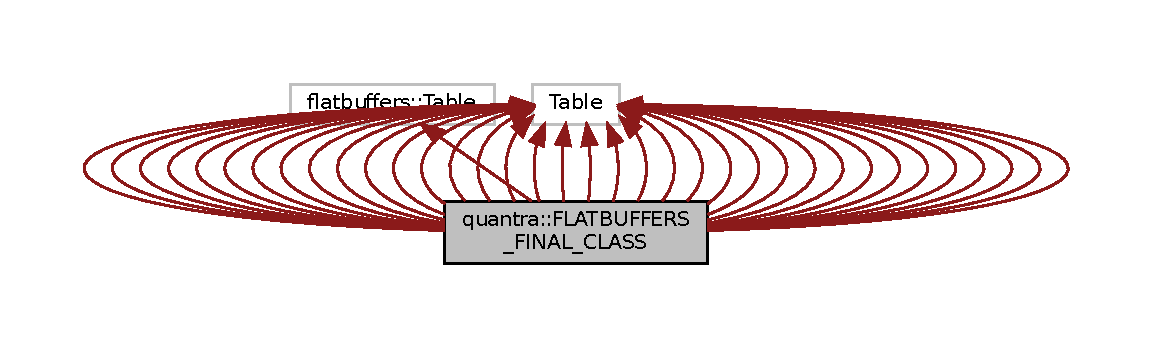
\includegraphics[width=350pt]{structquantra_1_1FLATBUFFERS__FINAL__CLASS__inherit__graph}
\end{center}
\end{figure}


Collaboration diagram for quantra\+:\+:F\+L\+A\+T\+B\+U\+F\+F\+E\+R\+S\+\_\+\+F\+I\+N\+A\+L\+\_\+\+C\+L\+A\+SS\+:\nopagebreak
\begin{figure}[H]
\begin{center}
\leavevmode
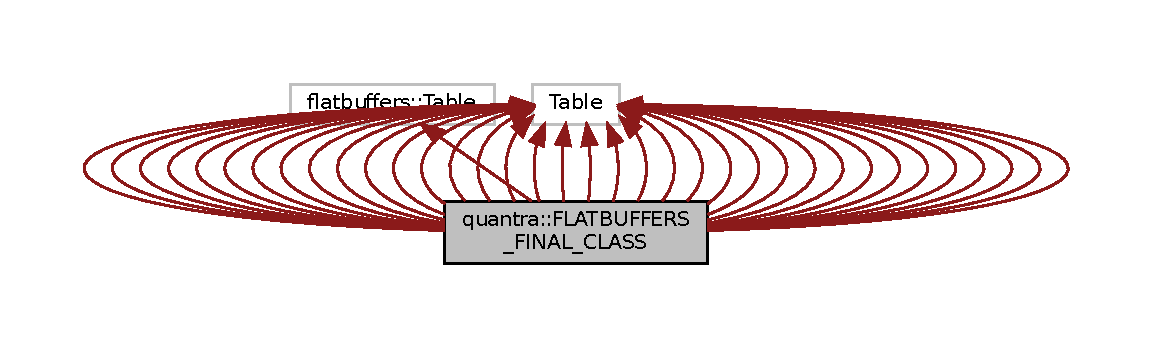
\includegraphics[width=350pt]{structquantra_1_1FLATBUFFERS__FINAL__CLASS__coll__graph}
\end{center}
\end{figure}
\subsection*{Public Types}
\begin{DoxyCompactItemize}
\item 
\mbox{\Hypertarget{structquantra_1_1FLATBUFFERS__FINAL__CLASS_aee1088c5dfd4144715b78d5078d1f010}\label{structquantra_1_1FLATBUFFERS__FINAL__CLASS_aee1088c5dfd4144715b78d5078d1f010}} 
typedef \hyperlink{structquantra_1_1YieldBuilder}{Yield\+Builder} {\bfseries Builder}
\item 
\mbox{\Hypertarget{structquantra_1_1FLATBUFFERS__FINAL__CLASS_a311957de23fcefb4a41c580ddc122497}\label{structquantra_1_1FLATBUFFERS__FINAL__CLASS_a311957de23fcefb4a41c580ddc122497}} 
typedef \hyperlink{structquantra_1_1PricingBuilder}{Pricing\+Builder} {\bfseries Builder}
\item 
\mbox{\Hypertarget{structquantra_1_1FLATBUFFERS__FINAL__CLASS_a76625e1e2e92b2474d14f19fd52bedc1}\label{structquantra_1_1FLATBUFFERS__FINAL__CLASS_a76625e1e2e92b2474d14f19fd52bedc1}} 
typedef \hyperlink{structquantra_1_1ErrorBuilder}{Error\+Builder} {\bfseries Builder}
\item 
\mbox{\Hypertarget{structquantra_1_1FLATBUFFERS__FINAL__CLASS_a843cf4218cff3a165ff02856dda212b0}\label{structquantra_1_1FLATBUFFERS__FINAL__CLASS_a843cf4218cff3a165ff02856dda212b0}} 
typedef \hyperlink{structquantra_1_1FixedRateBondBuilder}{Fixed\+Rate\+Bond\+Builder} {\bfseries Builder}
\item 
\mbox{\Hypertarget{structquantra_1_1FLATBUFFERS__FINAL__CLASS_a7c002f7daa8e2674c4e4f72b91021f89}\label{structquantra_1_1FLATBUFFERS__FINAL__CLASS_a7c002f7daa8e2674c4e4f72b91021f89}} 
typedef \hyperlink{structquantra_1_1FlowInterestBuilder}{Flow\+Interest\+Builder} {\bfseries Builder}
\item 
\mbox{\Hypertarget{structquantra_1_1FLATBUFFERS__FINAL__CLASS_a41afb4c71a07174ad4a0909f1f625b26}\label{structquantra_1_1FLATBUFFERS__FINAL__CLASS_a41afb4c71a07174ad4a0909f1f625b26}} 
typedef \hyperlink{structquantra_1_1FlowPastInterestBuilder}{Flow\+Past\+Interest\+Builder} {\bfseries Builder}
\item 
\mbox{\Hypertarget{structquantra_1_1FLATBUFFERS__FINAL__CLASS_ad512dbd14d2e9ad5a53d3b250c543d9b}\label{structquantra_1_1FLATBUFFERS__FINAL__CLASS_ad512dbd14d2e9ad5a53d3b250c543d9b}} 
typedef \hyperlink{structquantra_1_1FlowNotionalBuilder}{Flow\+Notional\+Builder} {\bfseries Builder}
\item 
\mbox{\Hypertarget{structquantra_1_1FLATBUFFERS__FINAL__CLASS_abe87a146dbc14d8d5bf81fce82d3ad24}\label{structquantra_1_1FLATBUFFERS__FINAL__CLASS_abe87a146dbc14d8d5bf81fce82d3ad24}} 
typedef \hyperlink{structquantra_1_1FlowsWrapperBuilder}{Flows\+Wrapper\+Builder} {\bfseries Builder}
\item 
\mbox{\Hypertarget{structquantra_1_1FLATBUFFERS__FINAL__CLASS_aa953af52fa6dd3e79ee3819e4fc9cc1f}\label{structquantra_1_1FLATBUFFERS__FINAL__CLASS_aa953af52fa6dd3e79ee3819e4fc9cc1f}} 
typedef \hyperlink{structquantra_1_1FixedRateBondResponseBuilder}{Fixed\+Rate\+Bond\+Response\+Builder} {\bfseries Builder}
\item 
\mbox{\Hypertarget{structquantra_1_1FLATBUFFERS__FINAL__CLASS_a7d042bcaa1a15c316b80cc5ed849f218}\label{structquantra_1_1FLATBUFFERS__FINAL__CLASS_a7d042bcaa1a15c316b80cc5ed849f218}} 
typedef \hyperlink{structquantra_1_1PriceFixedRateBondResponseBuilder}{Price\+Fixed\+Rate\+Bond\+Response\+Builder} {\bfseries Builder}
\item 
\mbox{\Hypertarget{structquantra_1_1FLATBUFFERS__FINAL__CLASS_a72a69f0988a1069bc67d78bbecce2e51}\label{structquantra_1_1FLATBUFFERS__FINAL__CLASS_a72a69f0988a1069bc67d78bbecce2e51}} 
typedef \hyperlink{structquantra_1_1FloatingRateBondBuilder}{Floating\+Rate\+Bond\+Builder} {\bfseries Builder}
\item 
\mbox{\Hypertarget{structquantra_1_1FLATBUFFERS__FINAL__CLASS_a7c002f7daa8e2674c4e4f72b91021f89}\label{structquantra_1_1FLATBUFFERS__FINAL__CLASS_a7c002f7daa8e2674c4e4f72b91021f89}} 
typedef \hyperlink{structquantra_1_1FlowInterestBuilder}{Flow\+Interest\+Builder} {\bfseries Builder}
\item 
\mbox{\Hypertarget{structquantra_1_1FLATBUFFERS__FINAL__CLASS_a41afb4c71a07174ad4a0909f1f625b26}\label{structquantra_1_1FLATBUFFERS__FINAL__CLASS_a41afb4c71a07174ad4a0909f1f625b26}} 
typedef \hyperlink{structquantra_1_1FlowPastInterestBuilder}{Flow\+Past\+Interest\+Builder} {\bfseries Builder}
\item 
\mbox{\Hypertarget{structquantra_1_1FLATBUFFERS__FINAL__CLASS_ad512dbd14d2e9ad5a53d3b250c543d9b}\label{structquantra_1_1FLATBUFFERS__FINAL__CLASS_ad512dbd14d2e9ad5a53d3b250c543d9b}} 
typedef \hyperlink{structquantra_1_1FlowNotionalBuilder}{Flow\+Notional\+Builder} {\bfseries Builder}
\item 
\mbox{\Hypertarget{structquantra_1_1FLATBUFFERS__FINAL__CLASS_abe87a146dbc14d8d5bf81fce82d3ad24}\label{structquantra_1_1FLATBUFFERS__FINAL__CLASS_abe87a146dbc14d8d5bf81fce82d3ad24}} 
typedef \hyperlink{structquantra_1_1FlowsWrapperBuilder}{Flows\+Wrapper\+Builder} {\bfseries Builder}
\item 
\mbox{\Hypertarget{structquantra_1_1FLATBUFFERS__FINAL__CLASS_aa953af52fa6dd3e79ee3819e4fc9cc1f}\label{structquantra_1_1FLATBUFFERS__FINAL__CLASS_aa953af52fa6dd3e79ee3819e4fc9cc1f}} 
typedef \hyperlink{structquantra_1_1FixedRateBondResponseBuilder}{Fixed\+Rate\+Bond\+Response\+Builder} {\bfseries Builder}
\item 
\mbox{\Hypertarget{structquantra_1_1FLATBUFFERS__FINAL__CLASS_a7d042bcaa1a15c316b80cc5ed849f218}\label{structquantra_1_1FLATBUFFERS__FINAL__CLASS_a7d042bcaa1a15c316b80cc5ed849f218}} 
typedef \hyperlink{structquantra_1_1PriceFixedRateBondResponseBuilder}{Price\+Fixed\+Rate\+Bond\+Response\+Builder} {\bfseries Builder}
\item 
\mbox{\Hypertarget{structquantra_1_1FLATBUFFERS__FINAL__CLASS_a213495e9dfbc74c1303eb5f3901f09f9}\label{structquantra_1_1FLATBUFFERS__FINAL__CLASS_a213495e9dfbc74c1303eb5f3901f09f9}} 
typedef \hyperlink{structquantra_1_1FixingBuilder}{Fixing\+Builder} {\bfseries Builder}
\item 
\mbox{\Hypertarget{structquantra_1_1FLATBUFFERS__FINAL__CLASS_ae0de3ee21571063dc0cae91027d658a6}\label{structquantra_1_1FLATBUFFERS__FINAL__CLASS_ae0de3ee21571063dc0cae91027d658a6}} 
typedef \hyperlink{structquantra_1_1IndexBuilder}{Index\+Builder} {\bfseries Builder}
\item 
\mbox{\Hypertarget{structquantra_1_1FLATBUFFERS__FINAL__CLASS_a78ae8cfc0e790122b2e2a2e4a4095000}\label{structquantra_1_1FLATBUFFERS__FINAL__CLASS_a78ae8cfc0e790122b2e2a2e4a4095000}} 
typedef \hyperlink{structquantra_1_1PriceFixedRateBondBuilder}{Price\+Fixed\+Rate\+Bond\+Builder} {\bfseries Builder}
\item 
\mbox{\Hypertarget{structquantra_1_1FLATBUFFERS__FINAL__CLASS_abba70d221e7086d1e9704f07b217eece}\label{structquantra_1_1FLATBUFFERS__FINAL__CLASS_abba70d221e7086d1e9704f07b217eece}} 
typedef \hyperlink{structquantra_1_1PriceFixedRateBondRequestBuilder}{Price\+Fixed\+Rate\+Bond\+Request\+Builder} {\bfseries Builder}
\item 
\mbox{\Hypertarget{structquantra_1_1FLATBUFFERS__FINAL__CLASS_ae251d213a5d464414f4f5cf40f5e10d8}\label{structquantra_1_1FLATBUFFERS__FINAL__CLASS_ae251d213a5d464414f4f5cf40f5e10d8}} 
typedef \hyperlink{structquantra_1_1PriceFloatingRateBondBuilder}{Price\+Floating\+Rate\+Bond\+Builder} {\bfseries Builder}
\item 
\mbox{\Hypertarget{structquantra_1_1FLATBUFFERS__FINAL__CLASS_aae2271061f24d7d6f15ab2af81f7798a}\label{structquantra_1_1FLATBUFFERS__FINAL__CLASS_aae2271061f24d7d6f15ab2af81f7798a}} 
typedef \hyperlink{structquantra_1_1PriceFloatingRateBondRequestBuilder}{Price\+Floating\+Rate\+Bond\+Request\+Builder} {\bfseries Builder}
\item 
\mbox{\Hypertarget{structquantra_1_1FLATBUFFERS__FINAL__CLASS_a7c002f7daa8e2674c4e4f72b91021f89}\label{structquantra_1_1FLATBUFFERS__FINAL__CLASS_a7c002f7daa8e2674c4e4f72b91021f89}} 
typedef \hyperlink{structquantra_1_1FlowInterestBuilder}{Flow\+Interest\+Builder} {\bfseries Builder}
\item 
\mbox{\Hypertarget{structquantra_1_1FLATBUFFERS__FINAL__CLASS_a41afb4c71a07174ad4a0909f1f625b26}\label{structquantra_1_1FLATBUFFERS__FINAL__CLASS_a41afb4c71a07174ad4a0909f1f625b26}} 
typedef \hyperlink{structquantra_1_1FlowPastInterestBuilder}{Flow\+Past\+Interest\+Builder} {\bfseries Builder}
\item 
\mbox{\Hypertarget{structquantra_1_1FLATBUFFERS__FINAL__CLASS_ad512dbd14d2e9ad5a53d3b250c543d9b}\label{structquantra_1_1FLATBUFFERS__FINAL__CLASS_ad512dbd14d2e9ad5a53d3b250c543d9b}} 
typedef \hyperlink{structquantra_1_1FlowNotionalBuilder}{Flow\+Notional\+Builder} {\bfseries Builder}
\item 
\mbox{\Hypertarget{structquantra_1_1FLATBUFFERS__FINAL__CLASS_abe87a146dbc14d8d5bf81fce82d3ad24}\label{structquantra_1_1FLATBUFFERS__FINAL__CLASS_abe87a146dbc14d8d5bf81fce82d3ad24}} 
typedef \hyperlink{structquantra_1_1FlowsWrapperBuilder}{Flows\+Wrapper\+Builder} {\bfseries Builder}
\item 
\mbox{\Hypertarget{structquantra_1_1FLATBUFFERS__FINAL__CLASS_aa953af52fa6dd3e79ee3819e4fc9cc1f}\label{structquantra_1_1FLATBUFFERS__FINAL__CLASS_aa953af52fa6dd3e79ee3819e4fc9cc1f}} 
typedef \hyperlink{structquantra_1_1FixedRateBondResponseBuilder}{Fixed\+Rate\+Bond\+Response\+Builder} {\bfseries Builder}
\item 
\mbox{\Hypertarget{structquantra_1_1FLATBUFFERS__FINAL__CLASS_a7d042bcaa1a15c316b80cc5ed849f218}\label{structquantra_1_1FLATBUFFERS__FINAL__CLASS_a7d042bcaa1a15c316b80cc5ed849f218}} 
typedef \hyperlink{structquantra_1_1PriceFixedRateBondResponseBuilder}{Price\+Fixed\+Rate\+Bond\+Response\+Builder} {\bfseries Builder}
\item 
\mbox{\Hypertarget{structquantra_1_1FLATBUFFERS__FINAL__CLASS_ac7d79b343bd4e7836e9e4f3f38432736}\label{structquantra_1_1FLATBUFFERS__FINAL__CLASS_ac7d79b343bd4e7836e9e4f3f38432736}} 
typedef \hyperlink{structquantra_1_1ScheduleBuilder}{Schedule\+Builder} {\bfseries Builder}
\item 
\mbox{\Hypertarget{structquantra_1_1FLATBUFFERS__FINAL__CLASS_a13d8984790d81e6fae58e393e6ce3b14}\label{structquantra_1_1FLATBUFFERS__FINAL__CLASS_a13d8984790d81e6fae58e393e6ce3b14}} 
typedef \hyperlink{structquantra_1_1DepositHelperBuilder}{Deposit\+Helper\+Builder} {\bfseries Builder}
\item 
\mbox{\Hypertarget{structquantra_1_1FLATBUFFERS__FINAL__CLASS_a0541aaf7739470f804385d8fa4669974}\label{structquantra_1_1FLATBUFFERS__FINAL__CLASS_a0541aaf7739470f804385d8fa4669974}} 
typedef \hyperlink{structquantra_1_1FRAHelperBuilder}{F\+R\+A\+Helper\+Builder} {\bfseries Builder}
\item 
\mbox{\Hypertarget{structquantra_1_1FLATBUFFERS__FINAL__CLASS_aadbc9bd6f7f4a812d42a37ff3bf4e64b}\label{structquantra_1_1FLATBUFFERS__FINAL__CLASS_aadbc9bd6f7f4a812d42a37ff3bf4e64b}} 
typedef \hyperlink{structquantra_1_1FutureHelperBuilder}{Future\+Helper\+Builder} {\bfseries Builder}
\item 
\mbox{\Hypertarget{structquantra_1_1FLATBUFFERS__FINAL__CLASS_a2e533587044dc5657c7e1f68eeaf1bf6}\label{structquantra_1_1FLATBUFFERS__FINAL__CLASS_a2e533587044dc5657c7e1f68eeaf1bf6}} 
typedef \hyperlink{structquantra_1_1SwapHelperBuilder}{Swap\+Helper\+Builder} {\bfseries Builder}
\item 
\mbox{\Hypertarget{structquantra_1_1FLATBUFFERS__FINAL__CLASS_a2fe8ad33ae30703c2dd84f7fce652ac6}\label{structquantra_1_1FLATBUFFERS__FINAL__CLASS_a2fe8ad33ae30703c2dd84f7fce652ac6}} 
typedef \hyperlink{structquantra_1_1BondHelperBuilder}{Bond\+Helper\+Builder} {\bfseries Builder}
\item 
\mbox{\Hypertarget{structquantra_1_1FLATBUFFERS__FINAL__CLASS_abcaecf566c2113f5daceb5f2cb608b43}\label{structquantra_1_1FLATBUFFERS__FINAL__CLASS_abcaecf566c2113f5daceb5f2cb608b43}} 
typedef \hyperlink{structquantra_1_1PointsWrapperBuilder}{Points\+Wrapper\+Builder} {\bfseries Builder}
\item 
\mbox{\Hypertarget{structquantra_1_1FLATBUFFERS__FINAL__CLASS_acff32b6cb800511b7093bbbf2e7ea8cf}\label{structquantra_1_1FLATBUFFERS__FINAL__CLASS_acff32b6cb800511b7093bbbf2e7ea8cf}} 
typedef \hyperlink{structquantra_1_1TermStructureBuilder}{Term\+Structure\+Builder} {\bfseries Builder}
\end{DoxyCompactItemize}
\subsection*{Public Member Functions}
\begin{DoxyCompactItemize}
\item 
\mbox{\Hypertarget{structquantra_1_1FLATBUFFERS__FINAL__CLASS_a955b9a33f908db3b82dea98242bc214e}\label{structquantra_1_1FLATBUFFERS__FINAL__CLASS_a955b9a33f908db3b82dea98242bc214e}} 
quantra\+::enums\+::\+Day\+Counter {\bfseries day\+\_\+counter} () const
\item 
\mbox{\Hypertarget{structquantra_1_1FLATBUFFERS__FINAL__CLASS_adba57dc42a842b5f450f4893d7400da1}\label{structquantra_1_1FLATBUFFERS__FINAL__CLASS_adba57dc42a842b5f450f4893d7400da1}} 
quantra\+::enums\+::\+Compounding {\bfseries compounding} () const
\item 
\mbox{\Hypertarget{structquantra_1_1FLATBUFFERS__FINAL__CLASS_a56f742df0ea6d251577d672eb4ae1a00}\label{structquantra_1_1FLATBUFFERS__FINAL__CLASS_a56f742df0ea6d251577d672eb4ae1a00}} 
quantra\+::enums\+::\+Frequency {\bfseries frequency} () const
\item 
\mbox{\Hypertarget{structquantra_1_1FLATBUFFERS__FINAL__CLASS_aed693ee5a45b5f53af7411f9cab6793a}\label{structquantra_1_1FLATBUFFERS__FINAL__CLASS_aed693ee5a45b5f53af7411f9cab6793a}} 
bool {\bfseries Verify} (flatbuffers\+::\+Verifier \&verifier) const
\item 
\mbox{\Hypertarget{structquantra_1_1FLATBUFFERS__FINAL__CLASS_a565651032145f0eb99a6f0c9b32d7fd0}\label{structquantra_1_1FLATBUFFERS__FINAL__CLASS_a565651032145f0eb99a6f0c9b32d7fd0}} 
const flatbuffers\+::\+String $\ast$ {\bfseries as\+\_\+of\+\_\+date} () const
\item 
\mbox{\Hypertarget{structquantra_1_1FLATBUFFERS__FINAL__CLASS_a7fa1e6060941ec462337605930e6f065}\label{structquantra_1_1FLATBUFFERS__FINAL__CLASS_a7fa1e6060941ec462337605930e6f065}} 
const flatbuffers\+::\+Vector$<$ flatbuffers\+::\+Offset$<$ quantra\+::\+Term\+Structure $>$ $>$ $\ast$ {\bfseries curves} () const
\item 
\mbox{\Hypertarget{structquantra_1_1FLATBUFFERS__FINAL__CLASS_a0a1bf5d6d7ca7114682a04f7ea41f7c7}\label{structquantra_1_1FLATBUFFERS__FINAL__CLASS_a0a1bf5d6d7ca7114682a04f7ea41f7c7}} 
bool {\bfseries bond\+\_\+pricing\+\_\+details} () const
\item 
\mbox{\Hypertarget{structquantra_1_1FLATBUFFERS__FINAL__CLASS_a5e7cf716a75e4cbc4911c9e6764c9edb}\label{structquantra_1_1FLATBUFFERS__FINAL__CLASS_a5e7cf716a75e4cbc4911c9e6764c9edb}} 
bool {\bfseries bond\+\_\+pricing\+\_\+flows} () const
\item 
\mbox{\Hypertarget{structquantra_1_1FLATBUFFERS__FINAL__CLASS_aed693ee5a45b5f53af7411f9cab6793a}\label{structquantra_1_1FLATBUFFERS__FINAL__CLASS_aed693ee5a45b5f53af7411f9cab6793a}} 
bool {\bfseries Verify} (flatbuffers\+::\+Verifier \&verifier) const
\item 
\mbox{\Hypertarget{structquantra_1_1FLATBUFFERS__FINAL__CLASS_a4fb1ac638f3b9744e24fab7b4242df96}\label{structquantra_1_1FLATBUFFERS__FINAL__CLASS_a4fb1ac638f3b9744e24fab7b4242df96}} 
const flatbuffers\+::\+String $\ast$ {\bfseries error\+\_\+message} () const
\item 
\mbox{\Hypertarget{structquantra_1_1FLATBUFFERS__FINAL__CLASS_aed693ee5a45b5f53af7411f9cab6793a}\label{structquantra_1_1FLATBUFFERS__FINAL__CLASS_aed693ee5a45b5f53af7411f9cab6793a}} 
bool {\bfseries Verify} (flatbuffers\+::\+Verifier \&verifier) const
\item 
\mbox{\Hypertarget{structquantra_1_1FLATBUFFERS__FINAL__CLASS_a2f95c4a4ab25cb17f5252fd7e6962827}\label{structquantra_1_1FLATBUFFERS__FINAL__CLASS_a2f95c4a4ab25cb17f5252fd7e6962827}} 
int32\+\_\+t {\bfseries settlement\+\_\+days} () const
\item 
\mbox{\Hypertarget{structquantra_1_1FLATBUFFERS__FINAL__CLASS_a18b1ae24369d0fda26e8523a2afb53de}\label{structquantra_1_1FLATBUFFERS__FINAL__CLASS_a18b1ae24369d0fda26e8523a2afb53de}} 
double {\bfseries face\+\_\+amount} () const
\item 
\mbox{\Hypertarget{structquantra_1_1FLATBUFFERS__FINAL__CLASS_a721326ea4afbe7a7cc21575f53f47324}\label{structquantra_1_1FLATBUFFERS__FINAL__CLASS_a721326ea4afbe7a7cc21575f53f47324}} 
double {\bfseries rate} () const
\item 
\mbox{\Hypertarget{structquantra_1_1FLATBUFFERS__FINAL__CLASS_ab03cf65ed2e6f70813f3bc9f43d2ca48}\label{structquantra_1_1FLATBUFFERS__FINAL__CLASS_ab03cf65ed2e6f70813f3bc9f43d2ca48}} 
quantra\+::enums\+::\+Day\+Counter {\bfseries accrual\+\_\+day\+\_\+counter} () const
\item 
\mbox{\Hypertarget{structquantra_1_1FLATBUFFERS__FINAL__CLASS_a01ba679cdd14fe10a620e64fe2fae6c2}\label{structquantra_1_1FLATBUFFERS__FINAL__CLASS_a01ba679cdd14fe10a620e64fe2fae6c2}} 
quantra\+::enums\+::\+Business\+Day\+Convention {\bfseries payment\+\_\+convention} () const
\item 
\mbox{\Hypertarget{structquantra_1_1FLATBUFFERS__FINAL__CLASS_a703292c01b0087fda51cd078d31ca15e}\label{structquantra_1_1FLATBUFFERS__FINAL__CLASS_a703292c01b0087fda51cd078d31ca15e}} 
double {\bfseries redemption} () const
\item 
\mbox{\Hypertarget{structquantra_1_1FLATBUFFERS__FINAL__CLASS_adf3517b162e1be9f52e6c0de30b15ab4}\label{structquantra_1_1FLATBUFFERS__FINAL__CLASS_adf3517b162e1be9f52e6c0de30b15ab4}} 
const flatbuffers\+::\+String $\ast$ {\bfseries issue\+\_\+date} () const
\item 
\mbox{\Hypertarget{structquantra_1_1FLATBUFFERS__FINAL__CLASS_a4980a75c547328bfac97fa23df17d655}\label{structquantra_1_1FLATBUFFERS__FINAL__CLASS_a4980a75c547328bfac97fa23df17d655}} 
const quantra\+::\+Schedule $\ast$ {\bfseries schedule} () const
\item 
\mbox{\Hypertarget{structquantra_1_1FLATBUFFERS__FINAL__CLASS_aed693ee5a45b5f53af7411f9cab6793a}\label{structquantra_1_1FLATBUFFERS__FINAL__CLASS_aed693ee5a45b5f53af7411f9cab6793a}} 
bool {\bfseries Verify} (flatbuffers\+::\+Verifier \&verifier) const
\item 
\mbox{\Hypertarget{structquantra_1_1FLATBUFFERS__FINAL__CLASS_a166da80825220ec9e04580d3aba13aca}\label{structquantra_1_1FLATBUFFERS__FINAL__CLASS_a166da80825220ec9e04580d3aba13aca}} 
double {\bfseries amount} () const
\item 
\mbox{\Hypertarget{structquantra_1_1FLATBUFFERS__FINAL__CLASS_add6840ddd841ee55494f311eb59a6af6}\label{structquantra_1_1FLATBUFFERS__FINAL__CLASS_add6840ddd841ee55494f311eb59a6af6}} 
const flatbuffers\+::\+String $\ast$ {\bfseries accrual\+\_\+start\+\_\+date} () const
\item 
\mbox{\Hypertarget{structquantra_1_1FLATBUFFERS__FINAL__CLASS_a9d0add6a4e2e5f6895c03c992fe74485}\label{structquantra_1_1FLATBUFFERS__FINAL__CLASS_a9d0add6a4e2e5f6895c03c992fe74485}} 
const flatbuffers\+::\+String $\ast$ {\bfseries accrual\+\_\+end\+\_\+date} () const
\item 
\mbox{\Hypertarget{structquantra_1_1FLATBUFFERS__FINAL__CLASS_aecb95f6e465c3d9921a452b43fade4ed}\label{structquantra_1_1FLATBUFFERS__FINAL__CLASS_aecb95f6e465c3d9921a452b43fade4ed}} 
float {\bfseries discount} () const
\item 
\mbox{\Hypertarget{structquantra_1_1FLATBUFFERS__FINAL__CLASS_aa5a25f3bfb8a4b4822cb5fcb1b479ff8}\label{structquantra_1_1FLATBUFFERS__FINAL__CLASS_aa5a25f3bfb8a4b4822cb5fcb1b479ff8}} 
float {\bfseries rate} () const
\item 
\mbox{\Hypertarget{structquantra_1_1FLATBUFFERS__FINAL__CLASS_afbd77034b48d3fee2f27dad0ac3503f1}\label{structquantra_1_1FLATBUFFERS__FINAL__CLASS_afbd77034b48d3fee2f27dad0ac3503f1}} 
float {\bfseries price} () const
\item 
\mbox{\Hypertarget{structquantra_1_1FLATBUFFERS__FINAL__CLASS_aed693ee5a45b5f53af7411f9cab6793a}\label{structquantra_1_1FLATBUFFERS__FINAL__CLASS_aed693ee5a45b5f53af7411f9cab6793a}} 
bool {\bfseries Verify} (flatbuffers\+::\+Verifier \&verifier) const
\item 
\mbox{\Hypertarget{structquantra_1_1FLATBUFFERS__FINAL__CLASS_a166da80825220ec9e04580d3aba13aca}\label{structquantra_1_1FLATBUFFERS__FINAL__CLASS_a166da80825220ec9e04580d3aba13aca}} 
double {\bfseries amount} () const
\item 
\mbox{\Hypertarget{structquantra_1_1FLATBUFFERS__FINAL__CLASS_add6840ddd841ee55494f311eb59a6af6}\label{structquantra_1_1FLATBUFFERS__FINAL__CLASS_add6840ddd841ee55494f311eb59a6af6}} 
const flatbuffers\+::\+String $\ast$ {\bfseries accrual\+\_\+start\+\_\+date} () const
\item 
\mbox{\Hypertarget{structquantra_1_1FLATBUFFERS__FINAL__CLASS_a9d0add6a4e2e5f6895c03c992fe74485}\label{structquantra_1_1FLATBUFFERS__FINAL__CLASS_a9d0add6a4e2e5f6895c03c992fe74485}} 
const flatbuffers\+::\+String $\ast$ {\bfseries accrual\+\_\+end\+\_\+date} () const
\item 
\mbox{\Hypertarget{structquantra_1_1FLATBUFFERS__FINAL__CLASS_aa5a25f3bfb8a4b4822cb5fcb1b479ff8}\label{structquantra_1_1FLATBUFFERS__FINAL__CLASS_aa5a25f3bfb8a4b4822cb5fcb1b479ff8}} 
float {\bfseries rate} () const
\item 
\mbox{\Hypertarget{structquantra_1_1FLATBUFFERS__FINAL__CLASS_aed693ee5a45b5f53af7411f9cab6793a}\label{structquantra_1_1FLATBUFFERS__FINAL__CLASS_aed693ee5a45b5f53af7411f9cab6793a}} 
bool {\bfseries Verify} (flatbuffers\+::\+Verifier \&verifier) const
\item 
\mbox{\Hypertarget{structquantra_1_1FLATBUFFERS__FINAL__CLASS_abe67178663d173c7a5da1e5ce47c2843}\label{structquantra_1_1FLATBUFFERS__FINAL__CLASS_abe67178663d173c7a5da1e5ce47c2843}} 
const flatbuffers\+::\+String $\ast$ {\bfseries date} () const
\item 
\mbox{\Hypertarget{structquantra_1_1FLATBUFFERS__FINAL__CLASS_a166da80825220ec9e04580d3aba13aca}\label{structquantra_1_1FLATBUFFERS__FINAL__CLASS_a166da80825220ec9e04580d3aba13aca}} 
double {\bfseries amount} () const
\item 
\mbox{\Hypertarget{structquantra_1_1FLATBUFFERS__FINAL__CLASS_aecb95f6e465c3d9921a452b43fade4ed}\label{structquantra_1_1FLATBUFFERS__FINAL__CLASS_aecb95f6e465c3d9921a452b43fade4ed}} 
float {\bfseries discount} () const
\item 
\mbox{\Hypertarget{structquantra_1_1FLATBUFFERS__FINAL__CLASS_afbd77034b48d3fee2f27dad0ac3503f1}\label{structquantra_1_1FLATBUFFERS__FINAL__CLASS_afbd77034b48d3fee2f27dad0ac3503f1}} 
float {\bfseries price} () const
\item 
\mbox{\Hypertarget{structquantra_1_1FLATBUFFERS__FINAL__CLASS_aed693ee5a45b5f53af7411f9cab6793a}\label{structquantra_1_1FLATBUFFERS__FINAL__CLASS_aed693ee5a45b5f53af7411f9cab6793a}} 
bool {\bfseries Verify} (flatbuffers\+::\+Verifier \&verifier) const
\item 
\mbox{\Hypertarget{structquantra_1_1FLATBUFFERS__FINAL__CLASS_ab95fb8e9407c2bda1637c5e48996ca37}\label{structquantra_1_1FLATBUFFERS__FINAL__CLASS_ab95fb8e9407c2bda1637c5e48996ca37}} 
quantra\+::\+Flow {\bfseries flow\+\_\+wrapper\+\_\+type} () const
\item 
\mbox{\Hypertarget{structquantra_1_1FLATBUFFERS__FINAL__CLASS_a1dca41a62b72f409dbfd6d27ab43aad1}\label{structquantra_1_1FLATBUFFERS__FINAL__CLASS_a1dca41a62b72f409dbfd6d27ab43aad1}} 
const void $\ast$ {\bfseries flow\+\_\+wrapper} () const
\item 
\mbox{\Hypertarget{structquantra_1_1FLATBUFFERS__FINAL__CLASS_a2225cfd4922352beac5604d8a00f46ef}\label{structquantra_1_1FLATBUFFERS__FINAL__CLASS_a2225cfd4922352beac5604d8a00f46ef}} 
{\footnotesize template$<$typename T $>$ }\\const T $\ast$ {\bfseries flow\+\_\+wrapper\+\_\+as} () const
\item 
\mbox{\Hypertarget{structquantra_1_1FLATBUFFERS__FINAL__CLASS_a90a09a81669c2966fc96de3c3e32757b}\label{structquantra_1_1FLATBUFFERS__FINAL__CLASS_a90a09a81669c2966fc96de3c3e32757b}} 
const quantra\+::\+Flow\+Interest $\ast$ {\bfseries flow\+\_\+wrapper\+\_\+as\+\_\+\+Flow\+Interest} () const
\item 
\mbox{\Hypertarget{structquantra_1_1FLATBUFFERS__FINAL__CLASS_a5abc9ea9cd01f6d33a1b75cd92e0cb09}\label{structquantra_1_1FLATBUFFERS__FINAL__CLASS_a5abc9ea9cd01f6d33a1b75cd92e0cb09}} 
const quantra\+::\+Flow\+Past\+Interest $\ast$ {\bfseries flow\+\_\+wrapper\+\_\+as\+\_\+\+Flow\+Past\+Interest} () const
\item 
\mbox{\Hypertarget{structquantra_1_1FLATBUFFERS__FINAL__CLASS_a2a1544e4ddf5c0ba47c8bc004f4963c3}\label{structquantra_1_1FLATBUFFERS__FINAL__CLASS_a2a1544e4ddf5c0ba47c8bc004f4963c3}} 
const quantra\+::\+Flow\+Notional $\ast$ {\bfseries flow\+\_\+wrapper\+\_\+as\+\_\+\+Flow\+Notional} () const
\item 
\mbox{\Hypertarget{structquantra_1_1FLATBUFFERS__FINAL__CLASS_aed693ee5a45b5f53af7411f9cab6793a}\label{structquantra_1_1FLATBUFFERS__FINAL__CLASS_aed693ee5a45b5f53af7411f9cab6793a}} 
bool {\bfseries Verify} (flatbuffers\+::\+Verifier \&verifier) const
\item 
\mbox{\Hypertarget{structquantra_1_1FLATBUFFERS__FINAL__CLASS_a3c5c36412aa6b8018c6e9293f8f7dbe9}\label{structquantra_1_1FLATBUFFERS__FINAL__CLASS_a3c5c36412aa6b8018c6e9293f8f7dbe9}} 
double {\bfseries npv} () const
\item 
\mbox{\Hypertarget{structquantra_1_1FLATBUFFERS__FINAL__CLASS_aedf3e4f110d0379f9d6ceffa31ba49e7}\label{structquantra_1_1FLATBUFFERS__FINAL__CLASS_aedf3e4f110d0379f9d6ceffa31ba49e7}} 
double {\bfseries clean\+\_\+price} () const
\item 
\mbox{\Hypertarget{structquantra_1_1FLATBUFFERS__FINAL__CLASS_a51261931153c996abe54368473b7fab2}\label{structquantra_1_1FLATBUFFERS__FINAL__CLASS_a51261931153c996abe54368473b7fab2}} 
double {\bfseries dirty\+\_\+price} () const
\item 
\mbox{\Hypertarget{structquantra_1_1FLATBUFFERS__FINAL__CLASS_a0643043a0955ed743ba0143c81e8328c}\label{structquantra_1_1FLATBUFFERS__FINAL__CLASS_a0643043a0955ed743ba0143c81e8328c}} 
double {\bfseries accrued\+\_\+amount} () const
\item 
\mbox{\Hypertarget{structquantra_1_1FLATBUFFERS__FINAL__CLASS_a842401d75722e096a4487010b128f8d4}\label{structquantra_1_1FLATBUFFERS__FINAL__CLASS_a842401d75722e096a4487010b128f8d4}} 
double {\bfseries yield} () const
\item 
\mbox{\Hypertarget{structquantra_1_1FLATBUFFERS__FINAL__CLASS_a90fe1e641ce101183f3e461986c117d3}\label{structquantra_1_1FLATBUFFERS__FINAL__CLASS_a90fe1e641ce101183f3e461986c117d3}} 
double {\bfseries accrued\+\_\+days} () const
\item 
\mbox{\Hypertarget{structquantra_1_1FLATBUFFERS__FINAL__CLASS_a1d59e2a282fc5d88f2c5bc6dd17d645d}\label{structquantra_1_1FLATBUFFERS__FINAL__CLASS_a1d59e2a282fc5d88f2c5bc6dd17d645d}} 
double {\bfseries macaulay\+\_\+duration} () const
\item 
\mbox{\Hypertarget{structquantra_1_1FLATBUFFERS__FINAL__CLASS_a1842a6a495702c8eb1741d7aa4720825}\label{structquantra_1_1FLATBUFFERS__FINAL__CLASS_a1842a6a495702c8eb1741d7aa4720825}} 
double {\bfseries modified\+\_\+duration} () const
\item 
\mbox{\Hypertarget{structquantra_1_1FLATBUFFERS__FINAL__CLASS_af391310ac92439c54d96f3d1de46f779}\label{structquantra_1_1FLATBUFFERS__FINAL__CLASS_af391310ac92439c54d96f3d1de46f779}} 
double {\bfseries convexity} () const
\item 
\mbox{\Hypertarget{structquantra_1_1FLATBUFFERS__FINAL__CLASS_a8678dc57d7507a5c42fb38f6e5e9d7be}\label{structquantra_1_1FLATBUFFERS__FINAL__CLASS_a8678dc57d7507a5c42fb38f6e5e9d7be}} 
double {\bfseries bps} () const
\item 
\mbox{\Hypertarget{structquantra_1_1FLATBUFFERS__FINAL__CLASS_aadf140966c400eb42ab77cc5049538a0}\label{structquantra_1_1FLATBUFFERS__FINAL__CLASS_aadf140966c400eb42ab77cc5049538a0}} 
const flatbuffers\+::\+Vector$<$ flatbuffers\+::\+Offset$<$ quantra\+::\+Flows\+Wrapper $>$ $>$ $\ast$ {\bfseries flows} () const
\item 
\mbox{\Hypertarget{structquantra_1_1FLATBUFFERS__FINAL__CLASS_aed693ee5a45b5f53af7411f9cab6793a}\label{structquantra_1_1FLATBUFFERS__FINAL__CLASS_aed693ee5a45b5f53af7411f9cab6793a}} 
bool {\bfseries Verify} (flatbuffers\+::\+Verifier \&verifier) const
\item 
\mbox{\Hypertarget{structquantra_1_1FLATBUFFERS__FINAL__CLASS_a12e5ea116142db128ca4e889ac5c752b}\label{structquantra_1_1FLATBUFFERS__FINAL__CLASS_a12e5ea116142db128ca4e889ac5c752b}} 
const flatbuffers\+::\+Vector$<$ flatbuffers\+::\+Offset$<$ quantra\+::\+Fixed\+Rate\+Bond\+Response $>$ $>$ $\ast$ {\bfseries bonds} () const
\item 
\mbox{\Hypertarget{structquantra_1_1FLATBUFFERS__FINAL__CLASS_aed693ee5a45b5f53af7411f9cab6793a}\label{structquantra_1_1FLATBUFFERS__FINAL__CLASS_aed693ee5a45b5f53af7411f9cab6793a}} 
bool {\bfseries Verify} (flatbuffers\+::\+Verifier \&verifier) const
\item 
\mbox{\Hypertarget{structquantra_1_1FLATBUFFERS__FINAL__CLASS_a2f95c4a4ab25cb17f5252fd7e6962827}\label{structquantra_1_1FLATBUFFERS__FINAL__CLASS_a2f95c4a4ab25cb17f5252fd7e6962827}} 
int32\+\_\+t {\bfseries settlement\+\_\+days} () const
\item 
\mbox{\Hypertarget{structquantra_1_1FLATBUFFERS__FINAL__CLASS_a18b1ae24369d0fda26e8523a2afb53de}\label{structquantra_1_1FLATBUFFERS__FINAL__CLASS_a18b1ae24369d0fda26e8523a2afb53de}} 
double {\bfseries face\+\_\+amount} () const
\item 
\mbox{\Hypertarget{structquantra_1_1FLATBUFFERS__FINAL__CLASS_a4980a75c547328bfac97fa23df17d655}\label{structquantra_1_1FLATBUFFERS__FINAL__CLASS_a4980a75c547328bfac97fa23df17d655}} 
const quantra\+::\+Schedule $\ast$ {\bfseries schedule} () const
\item 
\mbox{\Hypertarget{structquantra_1_1FLATBUFFERS__FINAL__CLASS_ae01144caafebbdbba931ba9e85f3da32}\label{structquantra_1_1FLATBUFFERS__FINAL__CLASS_ae01144caafebbdbba931ba9e85f3da32}} 
const quantra\+::\+Index $\ast$ {\bfseries index} () const
\item 
\mbox{\Hypertarget{structquantra_1_1FLATBUFFERS__FINAL__CLASS_ab03cf65ed2e6f70813f3bc9f43d2ca48}\label{structquantra_1_1FLATBUFFERS__FINAL__CLASS_ab03cf65ed2e6f70813f3bc9f43d2ca48}} 
quantra\+::enums\+::\+Day\+Counter {\bfseries accrual\+\_\+day\+\_\+counter} () const
\item 
\mbox{\Hypertarget{structquantra_1_1FLATBUFFERS__FINAL__CLASS_a01ba679cdd14fe10a620e64fe2fae6c2}\label{structquantra_1_1FLATBUFFERS__FINAL__CLASS_a01ba679cdd14fe10a620e64fe2fae6c2}} 
quantra\+::enums\+::\+Business\+Day\+Convention {\bfseries payment\+\_\+convention} () const
\item 
\mbox{\Hypertarget{structquantra_1_1FLATBUFFERS__FINAL__CLASS_af545a8a6ad48fc2a0597341e9ae68026}\label{structquantra_1_1FLATBUFFERS__FINAL__CLASS_af545a8a6ad48fc2a0597341e9ae68026}} 
int32\+\_\+t {\bfseries fixing\+\_\+days} () const
\item 
\mbox{\Hypertarget{structquantra_1_1FLATBUFFERS__FINAL__CLASS_afb98686c8dc5e287d93dfec7139013cd}\label{structquantra_1_1FLATBUFFERS__FINAL__CLASS_afb98686c8dc5e287d93dfec7139013cd}} 
double {\bfseries spread} () const
\item 
\mbox{\Hypertarget{structquantra_1_1FLATBUFFERS__FINAL__CLASS_ac05d204966d890512029f077dfdedcba}\label{structquantra_1_1FLATBUFFERS__FINAL__CLASS_ac05d204966d890512029f077dfdedcba}} 
bool {\bfseries in\+\_\+arrears} () const
\item 
\mbox{\Hypertarget{structquantra_1_1FLATBUFFERS__FINAL__CLASS_a703292c01b0087fda51cd078d31ca15e}\label{structquantra_1_1FLATBUFFERS__FINAL__CLASS_a703292c01b0087fda51cd078d31ca15e}} 
double {\bfseries redemption} () const
\item 
\mbox{\Hypertarget{structquantra_1_1FLATBUFFERS__FINAL__CLASS_adf3517b162e1be9f52e6c0de30b15ab4}\label{structquantra_1_1FLATBUFFERS__FINAL__CLASS_adf3517b162e1be9f52e6c0de30b15ab4}} 
const flatbuffers\+::\+String $\ast$ {\bfseries issue\+\_\+date} () const
\item 
\mbox{\Hypertarget{structquantra_1_1FLATBUFFERS__FINAL__CLASS_aed693ee5a45b5f53af7411f9cab6793a}\label{structquantra_1_1FLATBUFFERS__FINAL__CLASS_aed693ee5a45b5f53af7411f9cab6793a}} 
bool {\bfseries Verify} (flatbuffers\+::\+Verifier \&verifier) const
\item 
\mbox{\Hypertarget{structquantra_1_1FLATBUFFERS__FINAL__CLASS_a166da80825220ec9e04580d3aba13aca}\label{structquantra_1_1FLATBUFFERS__FINAL__CLASS_a166da80825220ec9e04580d3aba13aca}} 
double {\bfseries amount} () const
\item 
\mbox{\Hypertarget{structquantra_1_1FLATBUFFERS__FINAL__CLASS_a39c2480a4a44a603975f828bc3fab419}\label{structquantra_1_1FLATBUFFERS__FINAL__CLASS_a39c2480a4a44a603975f828bc3fab419}} 
const flatbuffers\+::\+String $\ast$ {\bfseries fixing\+\_\+date} () const
\item 
\mbox{\Hypertarget{structquantra_1_1FLATBUFFERS__FINAL__CLASS_add6840ddd841ee55494f311eb59a6af6}\label{structquantra_1_1FLATBUFFERS__FINAL__CLASS_add6840ddd841ee55494f311eb59a6af6}} 
const flatbuffers\+::\+String $\ast$ {\bfseries accrual\+\_\+start\+\_\+date} () const
\item 
\mbox{\Hypertarget{structquantra_1_1FLATBUFFERS__FINAL__CLASS_a9d0add6a4e2e5f6895c03c992fe74485}\label{structquantra_1_1FLATBUFFERS__FINAL__CLASS_a9d0add6a4e2e5f6895c03c992fe74485}} 
const flatbuffers\+::\+String $\ast$ {\bfseries accrual\+\_\+end\+\_\+date} () const
\item 
\mbox{\Hypertarget{structquantra_1_1FLATBUFFERS__FINAL__CLASS_aecb95f6e465c3d9921a452b43fade4ed}\label{structquantra_1_1FLATBUFFERS__FINAL__CLASS_aecb95f6e465c3d9921a452b43fade4ed}} 
float {\bfseries discount} () const
\item 
\mbox{\Hypertarget{structquantra_1_1FLATBUFFERS__FINAL__CLASS_aa5a25f3bfb8a4b4822cb5fcb1b479ff8}\label{structquantra_1_1FLATBUFFERS__FINAL__CLASS_aa5a25f3bfb8a4b4822cb5fcb1b479ff8}} 
float {\bfseries rate} () const
\item 
\mbox{\Hypertarget{structquantra_1_1FLATBUFFERS__FINAL__CLASS_afbd77034b48d3fee2f27dad0ac3503f1}\label{structquantra_1_1FLATBUFFERS__FINAL__CLASS_afbd77034b48d3fee2f27dad0ac3503f1}} 
float {\bfseries price} () const
\item 
\mbox{\Hypertarget{structquantra_1_1FLATBUFFERS__FINAL__CLASS_aed693ee5a45b5f53af7411f9cab6793a}\label{structquantra_1_1FLATBUFFERS__FINAL__CLASS_aed693ee5a45b5f53af7411f9cab6793a}} 
bool {\bfseries Verify} (flatbuffers\+::\+Verifier \&verifier) const
\item 
\mbox{\Hypertarget{structquantra_1_1FLATBUFFERS__FINAL__CLASS_a166da80825220ec9e04580d3aba13aca}\label{structquantra_1_1FLATBUFFERS__FINAL__CLASS_a166da80825220ec9e04580d3aba13aca}} 
double {\bfseries amount} () const
\item 
\mbox{\Hypertarget{structquantra_1_1FLATBUFFERS__FINAL__CLASS_a39c2480a4a44a603975f828bc3fab419}\label{structquantra_1_1FLATBUFFERS__FINAL__CLASS_a39c2480a4a44a603975f828bc3fab419}} 
const flatbuffers\+::\+String $\ast$ {\bfseries fixing\+\_\+date} () const
\item 
\mbox{\Hypertarget{structquantra_1_1FLATBUFFERS__FINAL__CLASS_add6840ddd841ee55494f311eb59a6af6}\label{structquantra_1_1FLATBUFFERS__FINAL__CLASS_add6840ddd841ee55494f311eb59a6af6}} 
const flatbuffers\+::\+String $\ast$ {\bfseries accrual\+\_\+start\+\_\+date} () const
\item 
\mbox{\Hypertarget{structquantra_1_1FLATBUFFERS__FINAL__CLASS_a9d0add6a4e2e5f6895c03c992fe74485}\label{structquantra_1_1FLATBUFFERS__FINAL__CLASS_a9d0add6a4e2e5f6895c03c992fe74485}} 
const flatbuffers\+::\+String $\ast$ {\bfseries accrual\+\_\+end\+\_\+date} () const
\item 
\mbox{\Hypertarget{structquantra_1_1FLATBUFFERS__FINAL__CLASS_aa5a25f3bfb8a4b4822cb5fcb1b479ff8}\label{structquantra_1_1FLATBUFFERS__FINAL__CLASS_aa5a25f3bfb8a4b4822cb5fcb1b479ff8}} 
float {\bfseries rate} () const
\item 
\mbox{\Hypertarget{structquantra_1_1FLATBUFFERS__FINAL__CLASS_aed693ee5a45b5f53af7411f9cab6793a}\label{structquantra_1_1FLATBUFFERS__FINAL__CLASS_aed693ee5a45b5f53af7411f9cab6793a}} 
bool {\bfseries Verify} (flatbuffers\+::\+Verifier \&verifier) const
\item 
\mbox{\Hypertarget{structquantra_1_1FLATBUFFERS__FINAL__CLASS_abe67178663d173c7a5da1e5ce47c2843}\label{structquantra_1_1FLATBUFFERS__FINAL__CLASS_abe67178663d173c7a5da1e5ce47c2843}} 
const flatbuffers\+::\+String $\ast$ {\bfseries date} () const
\item 
\mbox{\Hypertarget{structquantra_1_1FLATBUFFERS__FINAL__CLASS_a166da80825220ec9e04580d3aba13aca}\label{structquantra_1_1FLATBUFFERS__FINAL__CLASS_a166da80825220ec9e04580d3aba13aca}} 
double {\bfseries amount} () const
\item 
\mbox{\Hypertarget{structquantra_1_1FLATBUFFERS__FINAL__CLASS_aecb95f6e465c3d9921a452b43fade4ed}\label{structquantra_1_1FLATBUFFERS__FINAL__CLASS_aecb95f6e465c3d9921a452b43fade4ed}} 
float {\bfseries discount} () const
\item 
\mbox{\Hypertarget{structquantra_1_1FLATBUFFERS__FINAL__CLASS_afbd77034b48d3fee2f27dad0ac3503f1}\label{structquantra_1_1FLATBUFFERS__FINAL__CLASS_afbd77034b48d3fee2f27dad0ac3503f1}} 
float {\bfseries price} () const
\item 
\mbox{\Hypertarget{structquantra_1_1FLATBUFFERS__FINAL__CLASS_aed693ee5a45b5f53af7411f9cab6793a}\label{structquantra_1_1FLATBUFFERS__FINAL__CLASS_aed693ee5a45b5f53af7411f9cab6793a}} 
bool {\bfseries Verify} (flatbuffers\+::\+Verifier \&verifier) const
\item 
\mbox{\Hypertarget{structquantra_1_1FLATBUFFERS__FINAL__CLASS_ab95fb8e9407c2bda1637c5e48996ca37}\label{structquantra_1_1FLATBUFFERS__FINAL__CLASS_ab95fb8e9407c2bda1637c5e48996ca37}} 
quantra\+::\+Flow {\bfseries flow\+\_\+wrapper\+\_\+type} () const
\item 
\mbox{\Hypertarget{structquantra_1_1FLATBUFFERS__FINAL__CLASS_a1dca41a62b72f409dbfd6d27ab43aad1}\label{structquantra_1_1FLATBUFFERS__FINAL__CLASS_a1dca41a62b72f409dbfd6d27ab43aad1}} 
const void $\ast$ {\bfseries flow\+\_\+wrapper} () const
\item 
\mbox{\Hypertarget{structquantra_1_1FLATBUFFERS__FINAL__CLASS_a2225cfd4922352beac5604d8a00f46ef}\label{structquantra_1_1FLATBUFFERS__FINAL__CLASS_a2225cfd4922352beac5604d8a00f46ef}} 
{\footnotesize template$<$typename T $>$ }\\const T $\ast$ {\bfseries flow\+\_\+wrapper\+\_\+as} () const
\item 
\mbox{\Hypertarget{structquantra_1_1FLATBUFFERS__FINAL__CLASS_a90a09a81669c2966fc96de3c3e32757b}\label{structquantra_1_1FLATBUFFERS__FINAL__CLASS_a90a09a81669c2966fc96de3c3e32757b}} 
const quantra\+::\+Flow\+Interest $\ast$ {\bfseries flow\+\_\+wrapper\+\_\+as\+\_\+\+Flow\+Interest} () const
\item 
\mbox{\Hypertarget{structquantra_1_1FLATBUFFERS__FINAL__CLASS_a5abc9ea9cd01f6d33a1b75cd92e0cb09}\label{structquantra_1_1FLATBUFFERS__FINAL__CLASS_a5abc9ea9cd01f6d33a1b75cd92e0cb09}} 
const quantra\+::\+Flow\+Past\+Interest $\ast$ {\bfseries flow\+\_\+wrapper\+\_\+as\+\_\+\+Flow\+Past\+Interest} () const
\item 
\mbox{\Hypertarget{structquantra_1_1FLATBUFFERS__FINAL__CLASS_a2a1544e4ddf5c0ba47c8bc004f4963c3}\label{structquantra_1_1FLATBUFFERS__FINAL__CLASS_a2a1544e4ddf5c0ba47c8bc004f4963c3}} 
const quantra\+::\+Flow\+Notional $\ast$ {\bfseries flow\+\_\+wrapper\+\_\+as\+\_\+\+Flow\+Notional} () const
\item 
\mbox{\Hypertarget{structquantra_1_1FLATBUFFERS__FINAL__CLASS_aed693ee5a45b5f53af7411f9cab6793a}\label{structquantra_1_1FLATBUFFERS__FINAL__CLASS_aed693ee5a45b5f53af7411f9cab6793a}} 
bool {\bfseries Verify} (flatbuffers\+::\+Verifier \&verifier) const
\item 
\mbox{\Hypertarget{structquantra_1_1FLATBUFFERS__FINAL__CLASS_a3c5c36412aa6b8018c6e9293f8f7dbe9}\label{structquantra_1_1FLATBUFFERS__FINAL__CLASS_a3c5c36412aa6b8018c6e9293f8f7dbe9}} 
double {\bfseries npv} () const
\item 
\mbox{\Hypertarget{structquantra_1_1FLATBUFFERS__FINAL__CLASS_aedf3e4f110d0379f9d6ceffa31ba49e7}\label{structquantra_1_1FLATBUFFERS__FINAL__CLASS_aedf3e4f110d0379f9d6ceffa31ba49e7}} 
double {\bfseries clean\+\_\+price} () const
\item 
\mbox{\Hypertarget{structquantra_1_1FLATBUFFERS__FINAL__CLASS_a51261931153c996abe54368473b7fab2}\label{structquantra_1_1FLATBUFFERS__FINAL__CLASS_a51261931153c996abe54368473b7fab2}} 
double {\bfseries dirty\+\_\+price} () const
\item 
\mbox{\Hypertarget{structquantra_1_1FLATBUFFERS__FINAL__CLASS_a0643043a0955ed743ba0143c81e8328c}\label{structquantra_1_1FLATBUFFERS__FINAL__CLASS_a0643043a0955ed743ba0143c81e8328c}} 
double {\bfseries accrued\+\_\+amount} () const
\item 
\mbox{\Hypertarget{structquantra_1_1FLATBUFFERS__FINAL__CLASS_a842401d75722e096a4487010b128f8d4}\label{structquantra_1_1FLATBUFFERS__FINAL__CLASS_a842401d75722e096a4487010b128f8d4}} 
double {\bfseries yield} () const
\item 
\mbox{\Hypertarget{structquantra_1_1FLATBUFFERS__FINAL__CLASS_a90fe1e641ce101183f3e461986c117d3}\label{structquantra_1_1FLATBUFFERS__FINAL__CLASS_a90fe1e641ce101183f3e461986c117d3}} 
double {\bfseries accrued\+\_\+days} () const
\item 
\mbox{\Hypertarget{structquantra_1_1FLATBUFFERS__FINAL__CLASS_a1d59e2a282fc5d88f2c5bc6dd17d645d}\label{structquantra_1_1FLATBUFFERS__FINAL__CLASS_a1d59e2a282fc5d88f2c5bc6dd17d645d}} 
double {\bfseries macaulay\+\_\+duration} () const
\item 
\mbox{\Hypertarget{structquantra_1_1FLATBUFFERS__FINAL__CLASS_a1842a6a495702c8eb1741d7aa4720825}\label{structquantra_1_1FLATBUFFERS__FINAL__CLASS_a1842a6a495702c8eb1741d7aa4720825}} 
double {\bfseries modified\+\_\+duration} () const
\item 
\mbox{\Hypertarget{structquantra_1_1FLATBUFFERS__FINAL__CLASS_af391310ac92439c54d96f3d1de46f779}\label{structquantra_1_1FLATBUFFERS__FINAL__CLASS_af391310ac92439c54d96f3d1de46f779}} 
double {\bfseries convexity} () const
\item 
\mbox{\Hypertarget{structquantra_1_1FLATBUFFERS__FINAL__CLASS_a8678dc57d7507a5c42fb38f6e5e9d7be}\label{structquantra_1_1FLATBUFFERS__FINAL__CLASS_a8678dc57d7507a5c42fb38f6e5e9d7be}} 
double {\bfseries bps} () const
\item 
\mbox{\Hypertarget{structquantra_1_1FLATBUFFERS__FINAL__CLASS_aadf140966c400eb42ab77cc5049538a0}\label{structquantra_1_1FLATBUFFERS__FINAL__CLASS_aadf140966c400eb42ab77cc5049538a0}} 
const flatbuffers\+::\+Vector$<$ flatbuffers\+::\+Offset$<$ quantra\+::\+Flows\+Wrapper $>$ $>$ $\ast$ {\bfseries flows} () const
\item 
\mbox{\Hypertarget{structquantra_1_1FLATBUFFERS__FINAL__CLASS_aed693ee5a45b5f53af7411f9cab6793a}\label{structquantra_1_1FLATBUFFERS__FINAL__CLASS_aed693ee5a45b5f53af7411f9cab6793a}} 
bool {\bfseries Verify} (flatbuffers\+::\+Verifier \&verifier) const
\item 
\mbox{\Hypertarget{structquantra_1_1FLATBUFFERS__FINAL__CLASS_a12e5ea116142db128ca4e889ac5c752b}\label{structquantra_1_1FLATBUFFERS__FINAL__CLASS_a12e5ea116142db128ca4e889ac5c752b}} 
const flatbuffers\+::\+Vector$<$ flatbuffers\+::\+Offset$<$ quantra\+::\+Fixed\+Rate\+Bond\+Response $>$ $>$ $\ast$ {\bfseries bonds} () const
\item 
\mbox{\Hypertarget{structquantra_1_1FLATBUFFERS__FINAL__CLASS_aed693ee5a45b5f53af7411f9cab6793a}\label{structquantra_1_1FLATBUFFERS__FINAL__CLASS_aed693ee5a45b5f53af7411f9cab6793a}} 
bool {\bfseries Verify} (flatbuffers\+::\+Verifier \&verifier) const
\item 
\mbox{\Hypertarget{structquantra_1_1FLATBUFFERS__FINAL__CLASS_abe67178663d173c7a5da1e5ce47c2843}\label{structquantra_1_1FLATBUFFERS__FINAL__CLASS_abe67178663d173c7a5da1e5ce47c2843}} 
const flatbuffers\+::\+String $\ast$ {\bfseries date} () const
\item 
\mbox{\Hypertarget{structquantra_1_1FLATBUFFERS__FINAL__CLASS_aa5a25f3bfb8a4b4822cb5fcb1b479ff8}\label{structquantra_1_1FLATBUFFERS__FINAL__CLASS_aa5a25f3bfb8a4b4822cb5fcb1b479ff8}} 
float {\bfseries rate} () const
\item 
\mbox{\Hypertarget{structquantra_1_1FLATBUFFERS__FINAL__CLASS_aed693ee5a45b5f53af7411f9cab6793a}\label{structquantra_1_1FLATBUFFERS__FINAL__CLASS_aed693ee5a45b5f53af7411f9cab6793a}} 
bool {\bfseries Verify} (flatbuffers\+::\+Verifier \&verifier) const
\item 
\mbox{\Hypertarget{structquantra_1_1FLATBUFFERS__FINAL__CLASS_a2e523784cfd5189cd8065447cb8172fc}\label{structquantra_1_1FLATBUFFERS__FINAL__CLASS_a2e523784cfd5189cd8065447cb8172fc}} 
int32\+\_\+t {\bfseries period\+\_\+number} () const
\item 
\mbox{\Hypertarget{structquantra_1_1FLATBUFFERS__FINAL__CLASS_a3165de497c44c41af79b4e376a5b4b03}\label{structquantra_1_1FLATBUFFERS__FINAL__CLASS_a3165de497c44c41af79b4e376a5b4b03}} 
quantra\+::enums\+::\+Time\+Unit {\bfseries period\+\_\+time\+\_\+unit} () const
\item 
\mbox{\Hypertarget{structquantra_1_1FLATBUFFERS__FINAL__CLASS_a2f95c4a4ab25cb17f5252fd7e6962827}\label{structquantra_1_1FLATBUFFERS__FINAL__CLASS_a2f95c4a4ab25cb17f5252fd7e6962827}} 
int32\+\_\+t {\bfseries settlement\+\_\+days} () const
\item 
\mbox{\Hypertarget{structquantra_1_1FLATBUFFERS__FINAL__CLASS_a22bef2961bc16a42406e7b6c3d62a33e}\label{structquantra_1_1FLATBUFFERS__FINAL__CLASS_a22bef2961bc16a42406e7b6c3d62a33e}} 
quantra\+::enums\+::\+Calendar {\bfseries calendar} () const
\item 
\mbox{\Hypertarget{structquantra_1_1FLATBUFFERS__FINAL__CLASS_acc1afb278b3cf7c9923940b4704456f9}\label{structquantra_1_1FLATBUFFERS__FINAL__CLASS_acc1afb278b3cf7c9923940b4704456f9}} 
quantra\+::enums\+::\+Business\+Day\+Convention {\bfseries business\+\_\+day\+\_\+convention} () const
\item 
\mbox{\Hypertarget{structquantra_1_1FLATBUFFERS__FINAL__CLASS_abdb9fb60303f28fc766fc1ab7c9555d8}\label{structquantra_1_1FLATBUFFERS__FINAL__CLASS_abdb9fb60303f28fc766fc1ab7c9555d8}} 
bool {\bfseries end\+\_\+of\+\_\+month} () const
\item 
\mbox{\Hypertarget{structquantra_1_1FLATBUFFERS__FINAL__CLASS_a955b9a33f908db3b82dea98242bc214e}\label{structquantra_1_1FLATBUFFERS__FINAL__CLASS_a955b9a33f908db3b82dea98242bc214e}} 
quantra\+::enums\+::\+Day\+Counter {\bfseries day\+\_\+counter} () const
\item 
\mbox{\Hypertarget{structquantra_1_1FLATBUFFERS__FINAL__CLASS_ac0992a882fdf0e3cc1274853d9350dae}\label{structquantra_1_1FLATBUFFERS__FINAL__CLASS_ac0992a882fdf0e3cc1274853d9350dae}} 
const flatbuffers\+::\+Vector$<$ flatbuffers\+::\+Offset$<$ quantra\+::\+Fixing $>$ $>$ $\ast$ {\bfseries fixings} () const
\item 
\mbox{\Hypertarget{structquantra_1_1FLATBUFFERS__FINAL__CLASS_aed693ee5a45b5f53af7411f9cab6793a}\label{structquantra_1_1FLATBUFFERS__FINAL__CLASS_aed693ee5a45b5f53af7411f9cab6793a}} 
bool {\bfseries Verify} (flatbuffers\+::\+Verifier \&verifier) const
\item 
\mbox{\Hypertarget{structquantra_1_1FLATBUFFERS__FINAL__CLASS_a2c68c02ac4d96cdf9b7e24928f4702f1}\label{structquantra_1_1FLATBUFFERS__FINAL__CLASS_a2c68c02ac4d96cdf9b7e24928f4702f1}} 
const quantra\+::\+Fixed\+Rate\+Bond $\ast$ {\bfseries fixed\+\_\+rate\+\_\+bond} () const
\item 
\mbox{\Hypertarget{structquantra_1_1FLATBUFFERS__FINAL__CLASS_a81f3cfb641540405607a0804e95e0a93}\label{structquantra_1_1FLATBUFFERS__FINAL__CLASS_a81f3cfb641540405607a0804e95e0a93}} 
const flatbuffers\+::\+String $\ast$ {\bfseries discounting\+\_\+curve} () const
\item 
\mbox{\Hypertarget{structquantra_1_1FLATBUFFERS__FINAL__CLASS_adda837c430b8e761e469d0f6c244d902}\label{structquantra_1_1FLATBUFFERS__FINAL__CLASS_adda837c430b8e761e469d0f6c244d902}} 
const quantra\+::\+Yield $\ast$ {\bfseries yield} () const
\item 
\mbox{\Hypertarget{structquantra_1_1FLATBUFFERS__FINAL__CLASS_aed693ee5a45b5f53af7411f9cab6793a}\label{structquantra_1_1FLATBUFFERS__FINAL__CLASS_aed693ee5a45b5f53af7411f9cab6793a}} 
bool {\bfseries Verify} (flatbuffers\+::\+Verifier \&verifier) const
\item 
\mbox{\Hypertarget{structquantra_1_1FLATBUFFERS__FINAL__CLASS_a8e72b9cbbc3759570f15f834326dc962}\label{structquantra_1_1FLATBUFFERS__FINAL__CLASS_a8e72b9cbbc3759570f15f834326dc962}} 
const quantra\+::\+Pricing $\ast$ {\bfseries pricing} () const
\item 
\mbox{\Hypertarget{structquantra_1_1FLATBUFFERS__FINAL__CLASS_a62ab27da704bc7bbea4088aef5b1a73a}\label{structquantra_1_1FLATBUFFERS__FINAL__CLASS_a62ab27da704bc7bbea4088aef5b1a73a}} 
const flatbuffers\+::\+Vector$<$ flatbuffers\+::\+Offset$<$ quantra\+::\+Price\+Fixed\+Rate\+Bond $>$ $>$ $\ast$ {\bfseries bonds} () const
\item 
\mbox{\Hypertarget{structquantra_1_1FLATBUFFERS__FINAL__CLASS_aed693ee5a45b5f53af7411f9cab6793a}\label{structquantra_1_1FLATBUFFERS__FINAL__CLASS_aed693ee5a45b5f53af7411f9cab6793a}} 
bool {\bfseries Verify} (flatbuffers\+::\+Verifier \&verifier) const
\item 
\mbox{\Hypertarget{structquantra_1_1FLATBUFFERS__FINAL__CLASS_a0dd5dd7f5218d25cc51835f175809c89}\label{structquantra_1_1FLATBUFFERS__FINAL__CLASS_a0dd5dd7f5218d25cc51835f175809c89}} 
const quantra\+::\+Floating\+Rate\+Bond $\ast$ {\bfseries floating\+\_\+rate\+\_\+bond} () const
\item 
\mbox{\Hypertarget{structquantra_1_1FLATBUFFERS__FINAL__CLASS_a81f3cfb641540405607a0804e95e0a93}\label{structquantra_1_1FLATBUFFERS__FINAL__CLASS_a81f3cfb641540405607a0804e95e0a93}} 
const flatbuffers\+::\+String $\ast$ {\bfseries discounting\+\_\+curve} () const
\item 
\mbox{\Hypertarget{structquantra_1_1FLATBUFFERS__FINAL__CLASS_a4586b896a8c839f39c8cefa0b9058369}\label{structquantra_1_1FLATBUFFERS__FINAL__CLASS_a4586b896a8c839f39c8cefa0b9058369}} 
const flatbuffers\+::\+String $\ast$ {\bfseries forecasting\+\_\+curve} () const
\item 
\mbox{\Hypertarget{structquantra_1_1FLATBUFFERS__FINAL__CLASS_adda837c430b8e761e469d0f6c244d902}\label{structquantra_1_1FLATBUFFERS__FINAL__CLASS_adda837c430b8e761e469d0f6c244d902}} 
const quantra\+::\+Yield $\ast$ {\bfseries yield} () const
\item 
\mbox{\Hypertarget{structquantra_1_1FLATBUFFERS__FINAL__CLASS_aed693ee5a45b5f53af7411f9cab6793a}\label{structquantra_1_1FLATBUFFERS__FINAL__CLASS_aed693ee5a45b5f53af7411f9cab6793a}} 
bool {\bfseries Verify} (flatbuffers\+::\+Verifier \&verifier) const
\item 
\mbox{\Hypertarget{structquantra_1_1FLATBUFFERS__FINAL__CLASS_a8e72b9cbbc3759570f15f834326dc962}\label{structquantra_1_1FLATBUFFERS__FINAL__CLASS_a8e72b9cbbc3759570f15f834326dc962}} 
const quantra\+::\+Pricing $\ast$ {\bfseries pricing} () const
\item 
\mbox{\Hypertarget{structquantra_1_1FLATBUFFERS__FINAL__CLASS_a92286901d4ca5024d7bf293453adac9a}\label{structquantra_1_1FLATBUFFERS__FINAL__CLASS_a92286901d4ca5024d7bf293453adac9a}} 
const flatbuffers\+::\+Vector$<$ flatbuffers\+::\+Offset$<$ quantra\+::\+Price\+Floating\+Rate\+Bond $>$ $>$ $\ast$ {\bfseries bonds} () const
\item 
\mbox{\Hypertarget{structquantra_1_1FLATBUFFERS__FINAL__CLASS_aed693ee5a45b5f53af7411f9cab6793a}\label{structquantra_1_1FLATBUFFERS__FINAL__CLASS_aed693ee5a45b5f53af7411f9cab6793a}} 
bool {\bfseries Verify} (flatbuffers\+::\+Verifier \&verifier) const
\item 
\mbox{\Hypertarget{structquantra_1_1FLATBUFFERS__FINAL__CLASS_a166da80825220ec9e04580d3aba13aca}\label{structquantra_1_1FLATBUFFERS__FINAL__CLASS_a166da80825220ec9e04580d3aba13aca}} 
double {\bfseries amount} () const
\item 
\mbox{\Hypertarget{structquantra_1_1FLATBUFFERS__FINAL__CLASS_add6840ddd841ee55494f311eb59a6af6}\label{structquantra_1_1FLATBUFFERS__FINAL__CLASS_add6840ddd841ee55494f311eb59a6af6}} 
const flatbuffers\+::\+String $\ast$ {\bfseries accrual\+\_\+start\+\_\+date} () const
\item 
\mbox{\Hypertarget{structquantra_1_1FLATBUFFERS__FINAL__CLASS_a9d0add6a4e2e5f6895c03c992fe74485}\label{structquantra_1_1FLATBUFFERS__FINAL__CLASS_a9d0add6a4e2e5f6895c03c992fe74485}} 
const flatbuffers\+::\+String $\ast$ {\bfseries accrual\+\_\+end\+\_\+date} () const
\item 
\mbox{\Hypertarget{structquantra_1_1FLATBUFFERS__FINAL__CLASS_aecb95f6e465c3d9921a452b43fade4ed}\label{structquantra_1_1FLATBUFFERS__FINAL__CLASS_aecb95f6e465c3d9921a452b43fade4ed}} 
float {\bfseries discount} () const
\item 
\mbox{\Hypertarget{structquantra_1_1FLATBUFFERS__FINAL__CLASS_aa5a25f3bfb8a4b4822cb5fcb1b479ff8}\label{structquantra_1_1FLATBUFFERS__FINAL__CLASS_aa5a25f3bfb8a4b4822cb5fcb1b479ff8}} 
float {\bfseries rate} () const
\item 
\mbox{\Hypertarget{structquantra_1_1FLATBUFFERS__FINAL__CLASS_afbd77034b48d3fee2f27dad0ac3503f1}\label{structquantra_1_1FLATBUFFERS__FINAL__CLASS_afbd77034b48d3fee2f27dad0ac3503f1}} 
float {\bfseries price} () const
\item 
\mbox{\Hypertarget{structquantra_1_1FLATBUFFERS__FINAL__CLASS_aed693ee5a45b5f53af7411f9cab6793a}\label{structquantra_1_1FLATBUFFERS__FINAL__CLASS_aed693ee5a45b5f53af7411f9cab6793a}} 
bool {\bfseries Verify} (flatbuffers\+::\+Verifier \&verifier) const
\item 
\mbox{\Hypertarget{structquantra_1_1FLATBUFFERS__FINAL__CLASS_a166da80825220ec9e04580d3aba13aca}\label{structquantra_1_1FLATBUFFERS__FINAL__CLASS_a166da80825220ec9e04580d3aba13aca}} 
double {\bfseries amount} () const
\item 
\mbox{\Hypertarget{structquantra_1_1FLATBUFFERS__FINAL__CLASS_add6840ddd841ee55494f311eb59a6af6}\label{structquantra_1_1FLATBUFFERS__FINAL__CLASS_add6840ddd841ee55494f311eb59a6af6}} 
const flatbuffers\+::\+String $\ast$ {\bfseries accrual\+\_\+start\+\_\+date} () const
\item 
\mbox{\Hypertarget{structquantra_1_1FLATBUFFERS__FINAL__CLASS_a9d0add6a4e2e5f6895c03c992fe74485}\label{structquantra_1_1FLATBUFFERS__FINAL__CLASS_a9d0add6a4e2e5f6895c03c992fe74485}} 
const flatbuffers\+::\+String $\ast$ {\bfseries accrual\+\_\+end\+\_\+date} () const
\item 
\mbox{\Hypertarget{structquantra_1_1FLATBUFFERS__FINAL__CLASS_aa5a25f3bfb8a4b4822cb5fcb1b479ff8}\label{structquantra_1_1FLATBUFFERS__FINAL__CLASS_aa5a25f3bfb8a4b4822cb5fcb1b479ff8}} 
float {\bfseries rate} () const
\item 
\mbox{\Hypertarget{structquantra_1_1FLATBUFFERS__FINAL__CLASS_aed693ee5a45b5f53af7411f9cab6793a}\label{structquantra_1_1FLATBUFFERS__FINAL__CLASS_aed693ee5a45b5f53af7411f9cab6793a}} 
bool {\bfseries Verify} (flatbuffers\+::\+Verifier \&verifier) const
\item 
\mbox{\Hypertarget{structquantra_1_1FLATBUFFERS__FINAL__CLASS_abe67178663d173c7a5da1e5ce47c2843}\label{structquantra_1_1FLATBUFFERS__FINAL__CLASS_abe67178663d173c7a5da1e5ce47c2843}} 
const flatbuffers\+::\+String $\ast$ {\bfseries date} () const
\item 
\mbox{\Hypertarget{structquantra_1_1FLATBUFFERS__FINAL__CLASS_a166da80825220ec9e04580d3aba13aca}\label{structquantra_1_1FLATBUFFERS__FINAL__CLASS_a166da80825220ec9e04580d3aba13aca}} 
double {\bfseries amount} () const
\item 
\mbox{\Hypertarget{structquantra_1_1FLATBUFFERS__FINAL__CLASS_aecb95f6e465c3d9921a452b43fade4ed}\label{structquantra_1_1FLATBUFFERS__FINAL__CLASS_aecb95f6e465c3d9921a452b43fade4ed}} 
float {\bfseries discount} () const
\item 
\mbox{\Hypertarget{structquantra_1_1FLATBUFFERS__FINAL__CLASS_afbd77034b48d3fee2f27dad0ac3503f1}\label{structquantra_1_1FLATBUFFERS__FINAL__CLASS_afbd77034b48d3fee2f27dad0ac3503f1}} 
float {\bfseries price} () const
\item 
\mbox{\Hypertarget{structquantra_1_1FLATBUFFERS__FINAL__CLASS_aed693ee5a45b5f53af7411f9cab6793a}\label{structquantra_1_1FLATBUFFERS__FINAL__CLASS_aed693ee5a45b5f53af7411f9cab6793a}} 
bool {\bfseries Verify} (flatbuffers\+::\+Verifier \&verifier) const
\item 
\mbox{\Hypertarget{structquantra_1_1FLATBUFFERS__FINAL__CLASS_ab95fb8e9407c2bda1637c5e48996ca37}\label{structquantra_1_1FLATBUFFERS__FINAL__CLASS_ab95fb8e9407c2bda1637c5e48996ca37}} 
quantra\+::\+Flow {\bfseries flow\+\_\+wrapper\+\_\+type} () const
\item 
\mbox{\Hypertarget{structquantra_1_1FLATBUFFERS__FINAL__CLASS_a1dca41a62b72f409dbfd6d27ab43aad1}\label{structquantra_1_1FLATBUFFERS__FINAL__CLASS_a1dca41a62b72f409dbfd6d27ab43aad1}} 
const void $\ast$ {\bfseries flow\+\_\+wrapper} () const
\item 
\mbox{\Hypertarget{structquantra_1_1FLATBUFFERS__FINAL__CLASS_a2225cfd4922352beac5604d8a00f46ef}\label{structquantra_1_1FLATBUFFERS__FINAL__CLASS_a2225cfd4922352beac5604d8a00f46ef}} 
{\footnotesize template$<$typename T $>$ }\\const T $\ast$ {\bfseries flow\+\_\+wrapper\+\_\+as} () const
\item 
\mbox{\Hypertarget{structquantra_1_1FLATBUFFERS__FINAL__CLASS_a90a09a81669c2966fc96de3c3e32757b}\label{structquantra_1_1FLATBUFFERS__FINAL__CLASS_a90a09a81669c2966fc96de3c3e32757b}} 
const quantra\+::\+Flow\+Interest $\ast$ {\bfseries flow\+\_\+wrapper\+\_\+as\+\_\+\+Flow\+Interest} () const
\item 
\mbox{\Hypertarget{structquantra_1_1FLATBUFFERS__FINAL__CLASS_a5abc9ea9cd01f6d33a1b75cd92e0cb09}\label{structquantra_1_1FLATBUFFERS__FINAL__CLASS_a5abc9ea9cd01f6d33a1b75cd92e0cb09}} 
const quantra\+::\+Flow\+Past\+Interest $\ast$ {\bfseries flow\+\_\+wrapper\+\_\+as\+\_\+\+Flow\+Past\+Interest} () const
\item 
\mbox{\Hypertarget{structquantra_1_1FLATBUFFERS__FINAL__CLASS_a2a1544e4ddf5c0ba47c8bc004f4963c3}\label{structquantra_1_1FLATBUFFERS__FINAL__CLASS_a2a1544e4ddf5c0ba47c8bc004f4963c3}} 
const quantra\+::\+Flow\+Notional $\ast$ {\bfseries flow\+\_\+wrapper\+\_\+as\+\_\+\+Flow\+Notional} () const
\item 
\mbox{\Hypertarget{structquantra_1_1FLATBUFFERS__FINAL__CLASS_aed693ee5a45b5f53af7411f9cab6793a}\label{structquantra_1_1FLATBUFFERS__FINAL__CLASS_aed693ee5a45b5f53af7411f9cab6793a}} 
bool {\bfseries Verify} (flatbuffers\+::\+Verifier \&verifier) const
\item 
\mbox{\Hypertarget{structquantra_1_1FLATBUFFERS__FINAL__CLASS_a3c5c36412aa6b8018c6e9293f8f7dbe9}\label{structquantra_1_1FLATBUFFERS__FINAL__CLASS_a3c5c36412aa6b8018c6e9293f8f7dbe9}} 
double {\bfseries npv} () const
\item 
\mbox{\Hypertarget{structquantra_1_1FLATBUFFERS__FINAL__CLASS_aedf3e4f110d0379f9d6ceffa31ba49e7}\label{structquantra_1_1FLATBUFFERS__FINAL__CLASS_aedf3e4f110d0379f9d6ceffa31ba49e7}} 
double {\bfseries clean\+\_\+price} () const
\item 
\mbox{\Hypertarget{structquantra_1_1FLATBUFFERS__FINAL__CLASS_a51261931153c996abe54368473b7fab2}\label{structquantra_1_1FLATBUFFERS__FINAL__CLASS_a51261931153c996abe54368473b7fab2}} 
double {\bfseries dirty\+\_\+price} () const
\item 
\mbox{\Hypertarget{structquantra_1_1FLATBUFFERS__FINAL__CLASS_a0643043a0955ed743ba0143c81e8328c}\label{structquantra_1_1FLATBUFFERS__FINAL__CLASS_a0643043a0955ed743ba0143c81e8328c}} 
double {\bfseries accrued\+\_\+amount} () const
\item 
\mbox{\Hypertarget{structquantra_1_1FLATBUFFERS__FINAL__CLASS_a842401d75722e096a4487010b128f8d4}\label{structquantra_1_1FLATBUFFERS__FINAL__CLASS_a842401d75722e096a4487010b128f8d4}} 
double {\bfseries yield} () const
\item 
\mbox{\Hypertarget{structquantra_1_1FLATBUFFERS__FINAL__CLASS_a90fe1e641ce101183f3e461986c117d3}\label{structquantra_1_1FLATBUFFERS__FINAL__CLASS_a90fe1e641ce101183f3e461986c117d3}} 
double {\bfseries accrued\+\_\+days} () const
\item 
\mbox{\Hypertarget{structquantra_1_1FLATBUFFERS__FINAL__CLASS_a1d59e2a282fc5d88f2c5bc6dd17d645d}\label{structquantra_1_1FLATBUFFERS__FINAL__CLASS_a1d59e2a282fc5d88f2c5bc6dd17d645d}} 
double {\bfseries macaulay\+\_\+duration} () const
\item 
\mbox{\Hypertarget{structquantra_1_1FLATBUFFERS__FINAL__CLASS_a1842a6a495702c8eb1741d7aa4720825}\label{structquantra_1_1FLATBUFFERS__FINAL__CLASS_a1842a6a495702c8eb1741d7aa4720825}} 
double {\bfseries modified\+\_\+duration} () const
\item 
\mbox{\Hypertarget{structquantra_1_1FLATBUFFERS__FINAL__CLASS_af391310ac92439c54d96f3d1de46f779}\label{structquantra_1_1FLATBUFFERS__FINAL__CLASS_af391310ac92439c54d96f3d1de46f779}} 
double {\bfseries convexity} () const
\item 
\mbox{\Hypertarget{structquantra_1_1FLATBUFFERS__FINAL__CLASS_a8678dc57d7507a5c42fb38f6e5e9d7be}\label{structquantra_1_1FLATBUFFERS__FINAL__CLASS_a8678dc57d7507a5c42fb38f6e5e9d7be}} 
double {\bfseries bps} () const
\item 
\mbox{\Hypertarget{structquantra_1_1FLATBUFFERS__FINAL__CLASS_aadf140966c400eb42ab77cc5049538a0}\label{structquantra_1_1FLATBUFFERS__FINAL__CLASS_aadf140966c400eb42ab77cc5049538a0}} 
const flatbuffers\+::\+Vector$<$ flatbuffers\+::\+Offset$<$ quantra\+::\+Flows\+Wrapper $>$ $>$ $\ast$ {\bfseries flows} () const
\item 
\mbox{\Hypertarget{structquantra_1_1FLATBUFFERS__FINAL__CLASS_aed693ee5a45b5f53af7411f9cab6793a}\label{structquantra_1_1FLATBUFFERS__FINAL__CLASS_aed693ee5a45b5f53af7411f9cab6793a}} 
bool {\bfseries Verify} (flatbuffers\+::\+Verifier \&verifier) const
\item 
\mbox{\Hypertarget{structquantra_1_1FLATBUFFERS__FINAL__CLASS_a12e5ea116142db128ca4e889ac5c752b}\label{structquantra_1_1FLATBUFFERS__FINAL__CLASS_a12e5ea116142db128ca4e889ac5c752b}} 
const flatbuffers\+::\+Vector$<$ flatbuffers\+::\+Offset$<$ quantra\+::\+Fixed\+Rate\+Bond\+Response $>$ $>$ $\ast$ {\bfseries bonds} () const
\item 
\mbox{\Hypertarget{structquantra_1_1FLATBUFFERS__FINAL__CLASS_aed693ee5a45b5f53af7411f9cab6793a}\label{structquantra_1_1FLATBUFFERS__FINAL__CLASS_aed693ee5a45b5f53af7411f9cab6793a}} 
bool {\bfseries Verify} (flatbuffers\+::\+Verifier \&verifier) const
\item 
\mbox{\Hypertarget{structquantra_1_1FLATBUFFERS__FINAL__CLASS_a22bef2961bc16a42406e7b6c3d62a33e}\label{structquantra_1_1FLATBUFFERS__FINAL__CLASS_a22bef2961bc16a42406e7b6c3d62a33e}} 
quantra\+::enums\+::\+Calendar {\bfseries calendar} () const
\item 
\mbox{\Hypertarget{structquantra_1_1FLATBUFFERS__FINAL__CLASS_a122143580b74bd04c6b38d31044c9836}\label{structquantra_1_1FLATBUFFERS__FINAL__CLASS_a122143580b74bd04c6b38d31044c9836}} 
const flatbuffers\+::\+String $\ast$ {\bfseries effective\+\_\+date} () const
\item 
\mbox{\Hypertarget{structquantra_1_1FLATBUFFERS__FINAL__CLASS_a20d35ff63f6504b8c480e7495c92f4c0}\label{structquantra_1_1FLATBUFFERS__FINAL__CLASS_a20d35ff63f6504b8c480e7495c92f4c0}} 
const flatbuffers\+::\+String $\ast$ {\bfseries termination\+\_\+date} () const
\item 
\mbox{\Hypertarget{structquantra_1_1FLATBUFFERS__FINAL__CLASS_a56f742df0ea6d251577d672eb4ae1a00}\label{structquantra_1_1FLATBUFFERS__FINAL__CLASS_a56f742df0ea6d251577d672eb4ae1a00}} 
quantra\+::enums\+::\+Frequency {\bfseries frequency} () const
\item 
\mbox{\Hypertarget{structquantra_1_1FLATBUFFERS__FINAL__CLASS_a9aed3344e1ba628e7cbe9a1e62c53c97}\label{structquantra_1_1FLATBUFFERS__FINAL__CLASS_a9aed3344e1ba628e7cbe9a1e62c53c97}} 
quantra\+::enums\+::\+Business\+Day\+Convention {\bfseries convention} () const
\item 
\mbox{\Hypertarget{structquantra_1_1FLATBUFFERS__FINAL__CLASS_ae84453a225271d427f860b4a568ba5da}\label{structquantra_1_1FLATBUFFERS__FINAL__CLASS_ae84453a225271d427f860b4a568ba5da}} 
quantra\+::enums\+::\+Business\+Day\+Convention {\bfseries termination\+\_\+date\+\_\+convention} () const
\item 
\mbox{\Hypertarget{structquantra_1_1FLATBUFFERS__FINAL__CLASS_abdfcd290dfa885f10864e6443dd4dc11}\label{structquantra_1_1FLATBUFFERS__FINAL__CLASS_abdfcd290dfa885f10864e6443dd4dc11}} 
quantra\+::enums\+::\+Date\+Generation\+Rule {\bfseries date\+\_\+generation\+\_\+rule} () const
\item 
\mbox{\Hypertarget{structquantra_1_1FLATBUFFERS__FINAL__CLASS_a4b9c21859e17ec63a2964bac8055bf96}\label{structquantra_1_1FLATBUFFERS__FINAL__CLASS_a4b9c21859e17ec63a2964bac8055bf96}} 
bool {\bfseries end\+\_\+of\+\_\+mont} () const
\item 
\mbox{\Hypertarget{structquantra_1_1FLATBUFFERS__FINAL__CLASS_aed693ee5a45b5f53af7411f9cab6793a}\label{structquantra_1_1FLATBUFFERS__FINAL__CLASS_aed693ee5a45b5f53af7411f9cab6793a}} 
bool {\bfseries Verify} (flatbuffers\+::\+Verifier \&verifier) const
\item 
\mbox{\Hypertarget{structquantra_1_1FLATBUFFERS__FINAL__CLASS_aa5a25f3bfb8a4b4822cb5fcb1b479ff8}\label{structquantra_1_1FLATBUFFERS__FINAL__CLASS_aa5a25f3bfb8a4b4822cb5fcb1b479ff8}} 
float {\bfseries rate} () const
\item 
\mbox{\Hypertarget{structquantra_1_1FLATBUFFERS__FINAL__CLASS_ab4ab050747fb985c5b2628688cc3658d}\label{structquantra_1_1FLATBUFFERS__FINAL__CLASS_ab4ab050747fb985c5b2628688cc3658d}} 
quantra\+::enums\+::\+Time\+Unit {\bfseries tenor\+\_\+time\+\_\+unit} () const
\item 
\mbox{\Hypertarget{structquantra_1_1FLATBUFFERS__FINAL__CLASS_a6da14d412a4e94b493875c800389e10e}\label{structquantra_1_1FLATBUFFERS__FINAL__CLASS_a6da14d412a4e94b493875c800389e10e}} 
int32\+\_\+t {\bfseries tenor\+\_\+number} () const
\item 
\mbox{\Hypertarget{structquantra_1_1FLATBUFFERS__FINAL__CLASS_af545a8a6ad48fc2a0597341e9ae68026}\label{structquantra_1_1FLATBUFFERS__FINAL__CLASS_af545a8a6ad48fc2a0597341e9ae68026}} 
int32\+\_\+t {\bfseries fixing\+\_\+days} () const
\item 
\mbox{\Hypertarget{structquantra_1_1FLATBUFFERS__FINAL__CLASS_a22bef2961bc16a42406e7b6c3d62a33e}\label{structquantra_1_1FLATBUFFERS__FINAL__CLASS_a22bef2961bc16a42406e7b6c3d62a33e}} 
quantra\+::enums\+::\+Calendar {\bfseries calendar} () const
\item 
\mbox{\Hypertarget{structquantra_1_1FLATBUFFERS__FINAL__CLASS_acc1afb278b3cf7c9923940b4704456f9}\label{structquantra_1_1FLATBUFFERS__FINAL__CLASS_acc1afb278b3cf7c9923940b4704456f9}} 
quantra\+::enums\+::\+Business\+Day\+Convention {\bfseries business\+\_\+day\+\_\+convention} () const
\item 
\mbox{\Hypertarget{structquantra_1_1FLATBUFFERS__FINAL__CLASS_a955b9a33f908db3b82dea98242bc214e}\label{structquantra_1_1FLATBUFFERS__FINAL__CLASS_a955b9a33f908db3b82dea98242bc214e}} 
quantra\+::enums\+::\+Day\+Counter {\bfseries day\+\_\+counter} () const
\item 
\mbox{\Hypertarget{structquantra_1_1FLATBUFFERS__FINAL__CLASS_aed693ee5a45b5f53af7411f9cab6793a}\label{structquantra_1_1FLATBUFFERS__FINAL__CLASS_aed693ee5a45b5f53af7411f9cab6793a}} 
bool {\bfseries Verify} (flatbuffers\+::\+Verifier \&verifier) const
\item 
\mbox{\Hypertarget{structquantra_1_1FLATBUFFERS__FINAL__CLASS_aa5a25f3bfb8a4b4822cb5fcb1b479ff8}\label{structquantra_1_1FLATBUFFERS__FINAL__CLASS_aa5a25f3bfb8a4b4822cb5fcb1b479ff8}} 
float {\bfseries rate} () const
\item 
\mbox{\Hypertarget{structquantra_1_1FLATBUFFERS__FINAL__CLASS_a80fe5cc4c8f09aaae93acf06dfaf07ab}\label{structquantra_1_1FLATBUFFERS__FINAL__CLASS_a80fe5cc4c8f09aaae93acf06dfaf07ab}} 
int32\+\_\+t {\bfseries months\+\_\+to\+\_\+start} () const
\item 
\mbox{\Hypertarget{structquantra_1_1FLATBUFFERS__FINAL__CLASS_abd8d071266371cb70216d1a6abb3c42d}\label{structquantra_1_1FLATBUFFERS__FINAL__CLASS_abd8d071266371cb70216d1a6abb3c42d}} 
int32\+\_\+t {\bfseries months\+\_\+to\+\_\+end} () const
\item 
\mbox{\Hypertarget{structquantra_1_1FLATBUFFERS__FINAL__CLASS_af545a8a6ad48fc2a0597341e9ae68026}\label{structquantra_1_1FLATBUFFERS__FINAL__CLASS_af545a8a6ad48fc2a0597341e9ae68026}} 
int32\+\_\+t {\bfseries fixing\+\_\+days} () const
\item 
\mbox{\Hypertarget{structquantra_1_1FLATBUFFERS__FINAL__CLASS_a22bef2961bc16a42406e7b6c3d62a33e}\label{structquantra_1_1FLATBUFFERS__FINAL__CLASS_a22bef2961bc16a42406e7b6c3d62a33e}} 
quantra\+::enums\+::\+Calendar {\bfseries calendar} () const
\item 
\mbox{\Hypertarget{structquantra_1_1FLATBUFFERS__FINAL__CLASS_acc1afb278b3cf7c9923940b4704456f9}\label{structquantra_1_1FLATBUFFERS__FINAL__CLASS_acc1afb278b3cf7c9923940b4704456f9}} 
quantra\+::enums\+::\+Business\+Day\+Convention {\bfseries business\+\_\+day\+\_\+convention} () const
\item 
\mbox{\Hypertarget{structquantra_1_1FLATBUFFERS__FINAL__CLASS_a955b9a33f908db3b82dea98242bc214e}\label{structquantra_1_1FLATBUFFERS__FINAL__CLASS_a955b9a33f908db3b82dea98242bc214e}} 
quantra\+::enums\+::\+Day\+Counter {\bfseries day\+\_\+counter} () const
\item 
\mbox{\Hypertarget{structquantra_1_1FLATBUFFERS__FINAL__CLASS_aed693ee5a45b5f53af7411f9cab6793a}\label{structquantra_1_1FLATBUFFERS__FINAL__CLASS_aed693ee5a45b5f53af7411f9cab6793a}} 
bool {\bfseries Verify} (flatbuffers\+::\+Verifier \&verifier) const
\item 
\mbox{\Hypertarget{structquantra_1_1FLATBUFFERS__FINAL__CLASS_aa5a25f3bfb8a4b4822cb5fcb1b479ff8}\label{structquantra_1_1FLATBUFFERS__FINAL__CLASS_aa5a25f3bfb8a4b4822cb5fcb1b479ff8}} 
float {\bfseries rate} () const
\item 
\mbox{\Hypertarget{structquantra_1_1FLATBUFFERS__FINAL__CLASS_a9993b32c191d96962b2964028f86d2b1}\label{structquantra_1_1FLATBUFFERS__FINAL__CLASS_a9993b32c191d96962b2964028f86d2b1}} 
const flatbuffers\+::\+String $\ast$ {\bfseries future\+\_\+start\+\_\+date} () const
\item 
\mbox{\Hypertarget{structquantra_1_1FLATBUFFERS__FINAL__CLASS_a8a47248aadc3df89fdd559fbe1bf414e}\label{structquantra_1_1FLATBUFFERS__FINAL__CLASS_a8a47248aadc3df89fdd559fbe1bf414e}} 
int32\+\_\+t {\bfseries future\+\_\+months} () const
\item 
\mbox{\Hypertarget{structquantra_1_1FLATBUFFERS__FINAL__CLASS_a22bef2961bc16a42406e7b6c3d62a33e}\label{structquantra_1_1FLATBUFFERS__FINAL__CLASS_a22bef2961bc16a42406e7b6c3d62a33e}} 
quantra\+::enums\+::\+Calendar {\bfseries calendar} () const
\item 
\mbox{\Hypertarget{structquantra_1_1FLATBUFFERS__FINAL__CLASS_acc1afb278b3cf7c9923940b4704456f9}\label{structquantra_1_1FLATBUFFERS__FINAL__CLASS_acc1afb278b3cf7c9923940b4704456f9}} 
quantra\+::enums\+::\+Business\+Day\+Convention {\bfseries business\+\_\+day\+\_\+convention} () const
\item 
\mbox{\Hypertarget{structquantra_1_1FLATBUFFERS__FINAL__CLASS_a955b9a33f908db3b82dea98242bc214e}\label{structquantra_1_1FLATBUFFERS__FINAL__CLASS_a955b9a33f908db3b82dea98242bc214e}} 
quantra\+::enums\+::\+Day\+Counter {\bfseries day\+\_\+counter} () const
\item 
\mbox{\Hypertarget{structquantra_1_1FLATBUFFERS__FINAL__CLASS_aed693ee5a45b5f53af7411f9cab6793a}\label{structquantra_1_1FLATBUFFERS__FINAL__CLASS_aed693ee5a45b5f53af7411f9cab6793a}} 
bool {\bfseries Verify} (flatbuffers\+::\+Verifier \&verifier) const
\item 
\mbox{\Hypertarget{structquantra_1_1FLATBUFFERS__FINAL__CLASS_aa5a25f3bfb8a4b4822cb5fcb1b479ff8}\label{structquantra_1_1FLATBUFFERS__FINAL__CLASS_aa5a25f3bfb8a4b4822cb5fcb1b479ff8}} 
float {\bfseries rate} () const
\item 
\mbox{\Hypertarget{structquantra_1_1FLATBUFFERS__FINAL__CLASS_ab4ab050747fb985c5b2628688cc3658d}\label{structquantra_1_1FLATBUFFERS__FINAL__CLASS_ab4ab050747fb985c5b2628688cc3658d}} 
quantra\+::enums\+::\+Time\+Unit {\bfseries tenor\+\_\+time\+\_\+unit} () const
\item 
\mbox{\Hypertarget{structquantra_1_1FLATBUFFERS__FINAL__CLASS_a6da14d412a4e94b493875c800389e10e}\label{structquantra_1_1FLATBUFFERS__FINAL__CLASS_a6da14d412a4e94b493875c800389e10e}} 
int32\+\_\+t {\bfseries tenor\+\_\+number} () const
\item 
\mbox{\Hypertarget{structquantra_1_1FLATBUFFERS__FINAL__CLASS_a22bef2961bc16a42406e7b6c3d62a33e}\label{structquantra_1_1FLATBUFFERS__FINAL__CLASS_a22bef2961bc16a42406e7b6c3d62a33e}} 
quantra\+::enums\+::\+Calendar {\bfseries calendar} () const
\item 
\mbox{\Hypertarget{structquantra_1_1FLATBUFFERS__FINAL__CLASS_a65434b34834bf4dbff94f974758b3ae3}\label{structquantra_1_1FLATBUFFERS__FINAL__CLASS_a65434b34834bf4dbff94f974758b3ae3}} 
quantra\+::enums\+::\+Frequency {\bfseries sw\+\_\+fixed\+\_\+leg\+\_\+frequency} () const
\item 
\mbox{\Hypertarget{structquantra_1_1FLATBUFFERS__FINAL__CLASS_a3812bb5013858730da8e79a4a8327413}\label{structquantra_1_1FLATBUFFERS__FINAL__CLASS_a3812bb5013858730da8e79a4a8327413}} 
quantra\+::enums\+::\+Business\+Day\+Convention {\bfseries sw\+\_\+fixed\+\_\+leg\+\_\+convention} () const
\item 
\mbox{\Hypertarget{structquantra_1_1FLATBUFFERS__FINAL__CLASS_ac8bc0ab2ac5d61c0d555856d187d150b}\label{structquantra_1_1FLATBUFFERS__FINAL__CLASS_ac8bc0ab2ac5d61c0d555856d187d150b}} 
quantra\+::enums\+::\+Day\+Counter {\bfseries sw\+\_\+fixed\+\_\+leg\+\_\+day\+\_\+counter} () const
\item 
\mbox{\Hypertarget{structquantra_1_1FLATBUFFERS__FINAL__CLASS_aeec4877bd50cf902509de636c47e7166}\label{structquantra_1_1FLATBUFFERS__FINAL__CLASS_aeec4877bd50cf902509de636c47e7166}} 
quantra\+::enums\+::\+Ibor {\bfseries sw\+\_\+floating\+\_\+leg\+\_\+index} () const
\item 
\mbox{\Hypertarget{structquantra_1_1FLATBUFFERS__FINAL__CLASS_a4653ad5df3a925e6588a0b6003cd51de}\label{structquantra_1_1FLATBUFFERS__FINAL__CLASS_a4653ad5df3a925e6588a0b6003cd51de}} 
float {\bfseries spread} () const
\item 
\mbox{\Hypertarget{structquantra_1_1FLATBUFFERS__FINAL__CLASS_a58bfec8d554367776ab0c308d1414be4}\label{structquantra_1_1FLATBUFFERS__FINAL__CLASS_a58bfec8d554367776ab0c308d1414be4}} 
int32\+\_\+t {\bfseries fwd\+\_\+start\+\_\+days} () const
\item 
\mbox{\Hypertarget{structquantra_1_1FLATBUFFERS__FINAL__CLASS_aed693ee5a45b5f53af7411f9cab6793a}\label{structquantra_1_1FLATBUFFERS__FINAL__CLASS_aed693ee5a45b5f53af7411f9cab6793a}} 
bool {\bfseries Verify} (flatbuffers\+::\+Verifier \&verifier) const
\item 
\mbox{\Hypertarget{structquantra_1_1FLATBUFFERS__FINAL__CLASS_aa5a25f3bfb8a4b4822cb5fcb1b479ff8}\label{structquantra_1_1FLATBUFFERS__FINAL__CLASS_aa5a25f3bfb8a4b4822cb5fcb1b479ff8}} 
float {\bfseries rate} () const
\item 
\mbox{\Hypertarget{structquantra_1_1FLATBUFFERS__FINAL__CLASS_a2f95c4a4ab25cb17f5252fd7e6962827}\label{structquantra_1_1FLATBUFFERS__FINAL__CLASS_a2f95c4a4ab25cb17f5252fd7e6962827}} 
int32\+\_\+t {\bfseries settlement\+\_\+days} () const
\item 
\mbox{\Hypertarget{structquantra_1_1FLATBUFFERS__FINAL__CLASS_a337f006a00696676f3a1521958276b25}\label{structquantra_1_1FLATBUFFERS__FINAL__CLASS_a337f006a00696676f3a1521958276b25}} 
float {\bfseries face\+\_\+amount} () const
\item 
\mbox{\Hypertarget{structquantra_1_1FLATBUFFERS__FINAL__CLASS_a4980a75c547328bfac97fa23df17d655}\label{structquantra_1_1FLATBUFFERS__FINAL__CLASS_a4980a75c547328bfac97fa23df17d655}} 
const quantra\+::\+Schedule $\ast$ {\bfseries schedule} () const
\item 
\mbox{\Hypertarget{structquantra_1_1FLATBUFFERS__FINAL__CLASS_aa2f146b82509ff6e744924f478f954e5}\label{structquantra_1_1FLATBUFFERS__FINAL__CLASS_aa2f146b82509ff6e744924f478f954e5}} 
float {\bfseries coupon\+\_\+rate} () const
\item 
\mbox{\Hypertarget{structquantra_1_1FLATBUFFERS__FINAL__CLASS_a955b9a33f908db3b82dea98242bc214e}\label{structquantra_1_1FLATBUFFERS__FINAL__CLASS_a955b9a33f908db3b82dea98242bc214e}} 
quantra\+::enums\+::\+Day\+Counter {\bfseries day\+\_\+counter} () const
\item 
\mbox{\Hypertarget{structquantra_1_1FLATBUFFERS__FINAL__CLASS_acc1afb278b3cf7c9923940b4704456f9}\label{structquantra_1_1FLATBUFFERS__FINAL__CLASS_acc1afb278b3cf7c9923940b4704456f9}} 
quantra\+::enums\+::\+Business\+Day\+Convention {\bfseries business\+\_\+day\+\_\+convention} () const
\item 
\mbox{\Hypertarget{structquantra_1_1FLATBUFFERS__FINAL__CLASS_a5d41c47e7e4513418d304c46ff663eb9}\label{structquantra_1_1FLATBUFFERS__FINAL__CLASS_a5d41c47e7e4513418d304c46ff663eb9}} 
float {\bfseries redemption} () const
\item 
\mbox{\Hypertarget{structquantra_1_1FLATBUFFERS__FINAL__CLASS_adf3517b162e1be9f52e6c0de30b15ab4}\label{structquantra_1_1FLATBUFFERS__FINAL__CLASS_adf3517b162e1be9f52e6c0de30b15ab4}} 
const flatbuffers\+::\+String $\ast$ {\bfseries issue\+\_\+date} () const
\item 
\mbox{\Hypertarget{structquantra_1_1FLATBUFFERS__FINAL__CLASS_aed693ee5a45b5f53af7411f9cab6793a}\label{structquantra_1_1FLATBUFFERS__FINAL__CLASS_aed693ee5a45b5f53af7411f9cab6793a}} 
bool {\bfseries Verify} (flatbuffers\+::\+Verifier \&verifier) const
\item 
\mbox{\Hypertarget{structquantra_1_1FLATBUFFERS__FINAL__CLASS_adcbe84e9f247a884dd9d5f7c1c8eab0d}\label{structquantra_1_1FLATBUFFERS__FINAL__CLASS_adcbe84e9f247a884dd9d5f7c1c8eab0d}} 
quantra\+::\+Point {\bfseries point\+\_\+wrapper\+\_\+type} () const
\item 
\mbox{\Hypertarget{structquantra_1_1FLATBUFFERS__FINAL__CLASS_a68a93717cad0ef23bea14144b5157eeb}\label{structquantra_1_1FLATBUFFERS__FINAL__CLASS_a68a93717cad0ef23bea14144b5157eeb}} 
const void $\ast$ {\bfseries point\+\_\+wrapper} () const
\item 
\mbox{\Hypertarget{structquantra_1_1FLATBUFFERS__FINAL__CLASS_a1f13a377e4fb1f0382a3f39a7a9fd560}\label{structquantra_1_1FLATBUFFERS__FINAL__CLASS_a1f13a377e4fb1f0382a3f39a7a9fd560}} 
{\footnotesize template$<$typename T $>$ }\\const T $\ast$ {\bfseries point\+\_\+wrapper\+\_\+as} () const
\item 
\mbox{\Hypertarget{structquantra_1_1FLATBUFFERS__FINAL__CLASS_af4a7ff31dcb20df1567267364d40b888}\label{structquantra_1_1FLATBUFFERS__FINAL__CLASS_af4a7ff31dcb20df1567267364d40b888}} 
const quantra\+::\+Deposit\+Helper $\ast$ {\bfseries point\+\_\+wrapper\+\_\+as\+\_\+\+Deposit\+Helper} () const
\item 
\mbox{\Hypertarget{structquantra_1_1FLATBUFFERS__FINAL__CLASS_a0ffb255a2ab81a871d9003e8e1619221}\label{structquantra_1_1FLATBUFFERS__FINAL__CLASS_a0ffb255a2ab81a871d9003e8e1619221}} 
const quantra\+::\+F\+R\+A\+Helper $\ast$ {\bfseries point\+\_\+wrapper\+\_\+as\+\_\+\+F\+R\+A\+Helper} () const
\item 
\mbox{\Hypertarget{structquantra_1_1FLATBUFFERS__FINAL__CLASS_a35cc0261551151481fa754391c49b0d1}\label{structquantra_1_1FLATBUFFERS__FINAL__CLASS_a35cc0261551151481fa754391c49b0d1}} 
const quantra\+::\+Future\+Helper $\ast$ {\bfseries point\+\_\+wrapper\+\_\+as\+\_\+\+Future\+Helper} () const
\item 
\mbox{\Hypertarget{structquantra_1_1FLATBUFFERS__FINAL__CLASS_a66eb9935141a52050f56736c7a000cc2}\label{structquantra_1_1FLATBUFFERS__FINAL__CLASS_a66eb9935141a52050f56736c7a000cc2}} 
const quantra\+::\+Swap\+Helper $\ast$ {\bfseries point\+\_\+wrapper\+\_\+as\+\_\+\+Swap\+Helper} () const
\item 
\mbox{\Hypertarget{structquantra_1_1FLATBUFFERS__FINAL__CLASS_ae48a884c17ce2dadeeb6bdd5fd03e7dc}\label{structquantra_1_1FLATBUFFERS__FINAL__CLASS_ae48a884c17ce2dadeeb6bdd5fd03e7dc}} 
const quantra\+::\+Bond\+Helper $\ast$ {\bfseries point\+\_\+wrapper\+\_\+as\+\_\+\+Bond\+Helper} () const
\item 
\mbox{\Hypertarget{structquantra_1_1FLATBUFFERS__FINAL__CLASS_aed693ee5a45b5f53af7411f9cab6793a}\label{structquantra_1_1FLATBUFFERS__FINAL__CLASS_aed693ee5a45b5f53af7411f9cab6793a}} 
bool {\bfseries Verify} (flatbuffers\+::\+Verifier \&verifier) const
\item 
\mbox{\Hypertarget{structquantra_1_1FLATBUFFERS__FINAL__CLASS_ae066b12c3333e4cd04b4ada7fd4ffda6}\label{structquantra_1_1FLATBUFFERS__FINAL__CLASS_ae066b12c3333e4cd04b4ada7fd4ffda6}} 
const flatbuffers\+::\+String $\ast$ {\bfseries id} () const
\item 
\mbox{\Hypertarget{structquantra_1_1FLATBUFFERS__FINAL__CLASS_a955b9a33f908db3b82dea98242bc214e}\label{structquantra_1_1FLATBUFFERS__FINAL__CLASS_a955b9a33f908db3b82dea98242bc214e}} 
quantra\+::enums\+::\+Day\+Counter {\bfseries day\+\_\+counter} () const
\item 
\mbox{\Hypertarget{structquantra_1_1FLATBUFFERS__FINAL__CLASS_a5a65a145ba6d887aaadc65f04f0f3672}\label{structquantra_1_1FLATBUFFERS__FINAL__CLASS_a5a65a145ba6d887aaadc65f04f0f3672}} 
quantra\+::enums\+::\+Interpolator {\bfseries interpolator} () const
\item 
\mbox{\Hypertarget{structquantra_1_1FLATBUFFERS__FINAL__CLASS_aa9bee89d88150e45bf9b731ed4d7b2c2}\label{structquantra_1_1FLATBUFFERS__FINAL__CLASS_aa9bee89d88150e45bf9b731ed4d7b2c2}} 
quantra\+::enums\+::\+Bootstrap\+Trait {\bfseries bootstrap\+\_\+trait} () const
\item 
\mbox{\Hypertarget{structquantra_1_1FLATBUFFERS__FINAL__CLASS_a60ed3de828a6359cd86219a5e7844de6}\label{structquantra_1_1FLATBUFFERS__FINAL__CLASS_a60ed3de828a6359cd86219a5e7844de6}} 
const flatbuffers\+::\+Vector$<$ flatbuffers\+::\+Offset$<$ quantra\+::\+Points\+Wrapper $>$ $>$ $\ast$ {\bfseries points} () const
\item 
\mbox{\Hypertarget{structquantra_1_1FLATBUFFERS__FINAL__CLASS_a565651032145f0eb99a6f0c9b32d7fd0}\label{structquantra_1_1FLATBUFFERS__FINAL__CLASS_a565651032145f0eb99a6f0c9b32d7fd0}} 
const flatbuffers\+::\+String $\ast$ {\bfseries as\+\_\+of\+\_\+date} () const
\item 
\mbox{\Hypertarget{structquantra_1_1FLATBUFFERS__FINAL__CLASS_aed693ee5a45b5f53af7411f9cab6793a}\label{structquantra_1_1FLATBUFFERS__FINAL__CLASS_aed693ee5a45b5f53af7411f9cab6793a}} 
bool {\bfseries Verify} (flatbuffers\+::\+Verifier \&verifier) const
\end{DoxyCompactItemize}


The documentation for this struct was generated from the following files\+:\begin{DoxyCompactItemize}
\item 
cpp/common\+\_\+generated.\+h\item 
cpp/fixed\+\_\+rate\+\_\+bond\+\_\+generated.\+h\item 
cpp/fixed\+\_\+rate\+\_\+bond\+\_\+response\+\_\+generated.\+h\item 
cpp/floating\+\_\+rate\+\_\+bond\+\_\+generated.\+h\item 
cpp/floating\+\_\+rate\+\_\+bond\+\_\+response\+\_\+generated.\+h\item 
cpp/index\+\_\+generated.\+h\item 
cpp/price\+\_\+fixed\+\_\+rate\+\_\+bond\+\_\+request\+\_\+generated.\+h\item 
cpp/price\+\_\+floating\+\_\+rate\+\_\+bond\+\_\+request\+\_\+generated.\+h\item 
cpp/responses\+\_\+generated.\+h\item 
cpp/schedule\+\_\+generated.\+h\item 
cpp/term\+\_\+structure\+\_\+generated.\+h\end{DoxyCompactItemize}

\hypertarget{structquantra_1_1FloatingRateBondBuilder}{}\section{quantra\+:\+:Floating\+Rate\+Bond\+Builder Struct Reference}
\label{structquantra_1_1FloatingRateBondBuilder}\index{quantra\+::\+Floating\+Rate\+Bond\+Builder@{quantra\+::\+Floating\+Rate\+Bond\+Builder}}
\subsection*{Public Types}
\begin{DoxyCompactItemize}
\item 
\mbox{\Hypertarget{structquantra_1_1FloatingRateBondBuilder_a7af2b364ca0034ad984c46566932d041}\label{structquantra_1_1FloatingRateBondBuilder_a7af2b364ca0034ad984c46566932d041}} 
typedef Floating\+Rate\+Bond {\bfseries Table}
\end{DoxyCompactItemize}
\subsection*{Public Member Functions}
\begin{DoxyCompactItemize}
\item 
\mbox{\Hypertarget{structquantra_1_1FloatingRateBondBuilder_a3800c5c9b935d4a7b9c9b73017997b31}\label{structquantra_1_1FloatingRateBondBuilder_a3800c5c9b935d4a7b9c9b73017997b31}} 
void {\bfseries add\+\_\+settlement\+\_\+days} (int32\+\_\+t settlement\+\_\+days)
\item 
\mbox{\Hypertarget{structquantra_1_1FloatingRateBondBuilder_a6de393ecdcdc3a12b123286d26493998}\label{structquantra_1_1FloatingRateBondBuilder_a6de393ecdcdc3a12b123286d26493998}} 
void {\bfseries add\+\_\+face\+\_\+amount} (double face\+\_\+amount)
\item 
\mbox{\Hypertarget{structquantra_1_1FloatingRateBondBuilder_a05342943e850d1993d7dfc80e1c65ce5}\label{structquantra_1_1FloatingRateBondBuilder_a05342943e850d1993d7dfc80e1c65ce5}} 
void {\bfseries add\+\_\+schedule} (flatbuffers\+::\+Offset$<$ quantra\+::\+Schedule $>$ schedule)
\item 
\mbox{\Hypertarget{structquantra_1_1FloatingRateBondBuilder_a56ad36f960fd41420cf58ef42503dbef}\label{structquantra_1_1FloatingRateBondBuilder_a56ad36f960fd41420cf58ef42503dbef}} 
void {\bfseries add\+\_\+index} (flatbuffers\+::\+Offset$<$ quantra\+::\+Index $>$ index)
\item 
\mbox{\Hypertarget{structquantra_1_1FloatingRateBondBuilder_ae9f691f5623bcc86b9efefc6d7d2a41c}\label{structquantra_1_1FloatingRateBondBuilder_ae9f691f5623bcc86b9efefc6d7d2a41c}} 
void {\bfseries add\+\_\+accrual\+\_\+day\+\_\+counter} (quantra\+::enums\+::\+Day\+Counter accrual\+\_\+day\+\_\+counter)
\item 
\mbox{\Hypertarget{structquantra_1_1FloatingRateBondBuilder_a602e5ff7ec78cddd2bf69ff1bf92dd12}\label{structquantra_1_1FloatingRateBondBuilder_a602e5ff7ec78cddd2bf69ff1bf92dd12}} 
void {\bfseries add\+\_\+payment\+\_\+convention} (quantra\+::enums\+::\+Business\+Day\+Convention payment\+\_\+convention)
\item 
\mbox{\Hypertarget{structquantra_1_1FloatingRateBondBuilder_ae8304a49d239526161bbc2e1416dcdf7}\label{structquantra_1_1FloatingRateBondBuilder_ae8304a49d239526161bbc2e1416dcdf7}} 
void {\bfseries add\+\_\+fixing\+\_\+days} (int32\+\_\+t fixing\+\_\+days)
\item 
\mbox{\Hypertarget{structquantra_1_1FloatingRateBondBuilder_a6479cf63ab42965017328f0e07b71cd0}\label{structquantra_1_1FloatingRateBondBuilder_a6479cf63ab42965017328f0e07b71cd0}} 
void {\bfseries add\+\_\+spread} (double spread)
\item 
\mbox{\Hypertarget{structquantra_1_1FloatingRateBondBuilder_ae9f5d90bc196c30812ea4634d5e0f7c4}\label{structquantra_1_1FloatingRateBondBuilder_ae9f5d90bc196c30812ea4634d5e0f7c4}} 
void {\bfseries add\+\_\+in\+\_\+arrears} (bool in\+\_\+arrears)
\item 
\mbox{\Hypertarget{structquantra_1_1FloatingRateBondBuilder_af228ba20947d6129769dd564b05e2763}\label{structquantra_1_1FloatingRateBondBuilder_af228ba20947d6129769dd564b05e2763}} 
void {\bfseries add\+\_\+redemption} (double redemption)
\item 
\mbox{\Hypertarget{structquantra_1_1FloatingRateBondBuilder_acc269eed75a0928a75f479ec3bdc3b5a}\label{structquantra_1_1FloatingRateBondBuilder_acc269eed75a0928a75f479ec3bdc3b5a}} 
void {\bfseries add\+\_\+issue\+\_\+date} (flatbuffers\+::\+Offset$<$ flatbuffers\+::\+String $>$ issue\+\_\+date)
\item 
\mbox{\Hypertarget{structquantra_1_1FloatingRateBondBuilder_a604f625dddad6fa363fc46869531b07e}\label{structquantra_1_1FloatingRateBondBuilder_a604f625dddad6fa363fc46869531b07e}} 
{\bfseries Floating\+Rate\+Bond\+Builder} (flatbuffers\+::\+Flat\+Buffer\+Builder \&\+\_\+fbb)
\item 
\mbox{\Hypertarget{structquantra_1_1FloatingRateBondBuilder_abe4770415d0f31ee551990f2a5b5d382}\label{structquantra_1_1FloatingRateBondBuilder_abe4770415d0f31ee551990f2a5b5d382}} 
flatbuffers\+::\+Offset$<$ Floating\+Rate\+Bond $>$ {\bfseries Finish} ()
\end{DoxyCompactItemize}
\subsection*{Public Attributes}
\begin{DoxyCompactItemize}
\item 
\mbox{\Hypertarget{structquantra_1_1FloatingRateBondBuilder_a8fb3e4e9f5955523a23ddbb1666798b3}\label{structquantra_1_1FloatingRateBondBuilder_a8fb3e4e9f5955523a23ddbb1666798b3}} 
flatbuffers\+::\+Flat\+Buffer\+Builder \& {\bfseries fbb\+\_\+}
\item 
\mbox{\Hypertarget{structquantra_1_1FloatingRateBondBuilder_aa0aebd5016f20d37c07cb453dd9da23f}\label{structquantra_1_1FloatingRateBondBuilder_aa0aebd5016f20d37c07cb453dd9da23f}} 
flatbuffers\+::uoffset\+\_\+t {\bfseries start\+\_\+}
\end{DoxyCompactItemize}


The documentation for this struct was generated from the following file\+:\begin{DoxyCompactItemize}
\item 
cpp/floating\+\_\+rate\+\_\+bond\+\_\+generated.\+h\end{DoxyCompactItemize}

\hypertarget{structquantra_1_1FlowInterestBuilder}{}\section{quantra\+:\+:Flow\+Interest\+Builder Struct Reference}
\label{structquantra_1_1FlowInterestBuilder}\index{quantra\+::\+Flow\+Interest\+Builder@{quantra\+::\+Flow\+Interest\+Builder}}
\subsection*{Public Types}
\begin{DoxyCompactItemize}
\item 
\mbox{\Hypertarget{structquantra_1_1FlowInterestBuilder_a14f7319d7c49222183871330e89b060c}\label{structquantra_1_1FlowInterestBuilder_a14f7319d7c49222183871330e89b060c}} 
typedef Flow\+Interest {\bfseries Table}
\item 
\mbox{\Hypertarget{structquantra_1_1FlowInterestBuilder_a14f7319d7c49222183871330e89b060c}\label{structquantra_1_1FlowInterestBuilder_a14f7319d7c49222183871330e89b060c}} 
typedef Flow\+Interest {\bfseries Table}
\item 
\mbox{\Hypertarget{structquantra_1_1FlowInterestBuilder_a14f7319d7c49222183871330e89b060c}\label{structquantra_1_1FlowInterestBuilder_a14f7319d7c49222183871330e89b060c}} 
typedef Flow\+Interest {\bfseries Table}
\end{DoxyCompactItemize}
\subsection*{Public Member Functions}
\begin{DoxyCompactItemize}
\item 
\mbox{\Hypertarget{structquantra_1_1FlowInterestBuilder_af7424059a3ce706b6b9aae705e19c1f8}\label{structquantra_1_1FlowInterestBuilder_af7424059a3ce706b6b9aae705e19c1f8}} 
void {\bfseries add\+\_\+amount} (double amount)
\item 
\mbox{\Hypertarget{structquantra_1_1FlowInterestBuilder_a32c5350de9c05ac7b675d48b8974c9f0}\label{structquantra_1_1FlowInterestBuilder_a32c5350de9c05ac7b675d48b8974c9f0}} 
void {\bfseries add\+\_\+accrual\+\_\+start\+\_\+date} (flatbuffers\+::\+Offset$<$ flatbuffers\+::\+String $>$ accrual\+\_\+start\+\_\+date)
\item 
\mbox{\Hypertarget{structquantra_1_1FlowInterestBuilder_a949f5c0ccf619f7c15e0c6ae6e6acb5b}\label{structquantra_1_1FlowInterestBuilder_a949f5c0ccf619f7c15e0c6ae6e6acb5b}} 
void {\bfseries add\+\_\+accrual\+\_\+end\+\_\+date} (flatbuffers\+::\+Offset$<$ flatbuffers\+::\+String $>$ accrual\+\_\+end\+\_\+date)
\item 
\mbox{\Hypertarget{structquantra_1_1FlowInterestBuilder_a1200efd055ba511bdabfbd2d5a9f3e29}\label{structquantra_1_1FlowInterestBuilder_a1200efd055ba511bdabfbd2d5a9f3e29}} 
void {\bfseries add\+\_\+discount} (float discount)
\item 
\mbox{\Hypertarget{structquantra_1_1FlowInterestBuilder_a2b35605c938c635d39748ccb58bed5c6}\label{structquantra_1_1FlowInterestBuilder_a2b35605c938c635d39748ccb58bed5c6}} 
void {\bfseries add\+\_\+rate} (float rate)
\item 
\mbox{\Hypertarget{structquantra_1_1FlowInterestBuilder_a4ee6a971fb7a04d64b7a5960dedad4df}\label{structquantra_1_1FlowInterestBuilder_a4ee6a971fb7a04d64b7a5960dedad4df}} 
void {\bfseries add\+\_\+price} (float price)
\item 
\mbox{\Hypertarget{structquantra_1_1FlowInterestBuilder_a28ec59385c7cf4ba22dcb2244faf6d25}\label{structquantra_1_1FlowInterestBuilder_a28ec59385c7cf4ba22dcb2244faf6d25}} 
{\bfseries Flow\+Interest\+Builder} (flatbuffers\+::\+Flat\+Buffer\+Builder \&\+\_\+fbb)
\item 
\mbox{\Hypertarget{structquantra_1_1FlowInterestBuilder_a9f628e0afe32f445bb1b3d5b1738cf9a}\label{structquantra_1_1FlowInterestBuilder_a9f628e0afe32f445bb1b3d5b1738cf9a}} 
flatbuffers\+::\+Offset$<$ Flow\+Interest $>$ {\bfseries Finish} ()
\item 
\mbox{\Hypertarget{structquantra_1_1FlowInterestBuilder_af7424059a3ce706b6b9aae705e19c1f8}\label{structquantra_1_1FlowInterestBuilder_af7424059a3ce706b6b9aae705e19c1f8}} 
void {\bfseries add\+\_\+amount} (double amount)
\item 
\mbox{\Hypertarget{structquantra_1_1FlowInterestBuilder_a8739b37ec33ac58038658ba76fce014a}\label{structquantra_1_1FlowInterestBuilder_a8739b37ec33ac58038658ba76fce014a}} 
void {\bfseries add\+\_\+fixing\+\_\+date} (flatbuffers\+::\+Offset$<$ flatbuffers\+::\+String $>$ fixing\+\_\+date)
\item 
\mbox{\Hypertarget{structquantra_1_1FlowInterestBuilder_a32c5350de9c05ac7b675d48b8974c9f0}\label{structquantra_1_1FlowInterestBuilder_a32c5350de9c05ac7b675d48b8974c9f0}} 
void {\bfseries add\+\_\+accrual\+\_\+start\+\_\+date} (flatbuffers\+::\+Offset$<$ flatbuffers\+::\+String $>$ accrual\+\_\+start\+\_\+date)
\item 
\mbox{\Hypertarget{structquantra_1_1FlowInterestBuilder_a949f5c0ccf619f7c15e0c6ae6e6acb5b}\label{structquantra_1_1FlowInterestBuilder_a949f5c0ccf619f7c15e0c6ae6e6acb5b}} 
void {\bfseries add\+\_\+accrual\+\_\+end\+\_\+date} (flatbuffers\+::\+Offset$<$ flatbuffers\+::\+String $>$ accrual\+\_\+end\+\_\+date)
\item 
\mbox{\Hypertarget{structquantra_1_1FlowInterestBuilder_a1200efd055ba511bdabfbd2d5a9f3e29}\label{structquantra_1_1FlowInterestBuilder_a1200efd055ba511bdabfbd2d5a9f3e29}} 
void {\bfseries add\+\_\+discount} (float discount)
\item 
\mbox{\Hypertarget{structquantra_1_1FlowInterestBuilder_a2b35605c938c635d39748ccb58bed5c6}\label{structquantra_1_1FlowInterestBuilder_a2b35605c938c635d39748ccb58bed5c6}} 
void {\bfseries add\+\_\+rate} (float rate)
\item 
\mbox{\Hypertarget{structquantra_1_1FlowInterestBuilder_a4ee6a971fb7a04d64b7a5960dedad4df}\label{structquantra_1_1FlowInterestBuilder_a4ee6a971fb7a04d64b7a5960dedad4df}} 
void {\bfseries add\+\_\+price} (float price)
\item 
\mbox{\Hypertarget{structquantra_1_1FlowInterestBuilder_a28ec59385c7cf4ba22dcb2244faf6d25}\label{structquantra_1_1FlowInterestBuilder_a28ec59385c7cf4ba22dcb2244faf6d25}} 
{\bfseries Flow\+Interest\+Builder} (flatbuffers\+::\+Flat\+Buffer\+Builder \&\+\_\+fbb)
\item 
\mbox{\Hypertarget{structquantra_1_1FlowInterestBuilder_a9f628e0afe32f445bb1b3d5b1738cf9a}\label{structquantra_1_1FlowInterestBuilder_a9f628e0afe32f445bb1b3d5b1738cf9a}} 
flatbuffers\+::\+Offset$<$ Flow\+Interest $>$ {\bfseries Finish} ()
\item 
\mbox{\Hypertarget{structquantra_1_1FlowInterestBuilder_af7424059a3ce706b6b9aae705e19c1f8}\label{structquantra_1_1FlowInterestBuilder_af7424059a3ce706b6b9aae705e19c1f8}} 
void {\bfseries add\+\_\+amount} (double amount)
\item 
\mbox{\Hypertarget{structquantra_1_1FlowInterestBuilder_a32c5350de9c05ac7b675d48b8974c9f0}\label{structquantra_1_1FlowInterestBuilder_a32c5350de9c05ac7b675d48b8974c9f0}} 
void {\bfseries add\+\_\+accrual\+\_\+start\+\_\+date} (flatbuffers\+::\+Offset$<$ flatbuffers\+::\+String $>$ accrual\+\_\+start\+\_\+date)
\item 
\mbox{\Hypertarget{structquantra_1_1FlowInterestBuilder_a949f5c0ccf619f7c15e0c6ae6e6acb5b}\label{structquantra_1_1FlowInterestBuilder_a949f5c0ccf619f7c15e0c6ae6e6acb5b}} 
void {\bfseries add\+\_\+accrual\+\_\+end\+\_\+date} (flatbuffers\+::\+Offset$<$ flatbuffers\+::\+String $>$ accrual\+\_\+end\+\_\+date)
\item 
\mbox{\Hypertarget{structquantra_1_1FlowInterestBuilder_a1200efd055ba511bdabfbd2d5a9f3e29}\label{structquantra_1_1FlowInterestBuilder_a1200efd055ba511bdabfbd2d5a9f3e29}} 
void {\bfseries add\+\_\+discount} (float discount)
\item 
\mbox{\Hypertarget{structquantra_1_1FlowInterestBuilder_a2b35605c938c635d39748ccb58bed5c6}\label{structquantra_1_1FlowInterestBuilder_a2b35605c938c635d39748ccb58bed5c6}} 
void {\bfseries add\+\_\+rate} (float rate)
\item 
\mbox{\Hypertarget{structquantra_1_1FlowInterestBuilder_a4ee6a971fb7a04d64b7a5960dedad4df}\label{structquantra_1_1FlowInterestBuilder_a4ee6a971fb7a04d64b7a5960dedad4df}} 
void {\bfseries add\+\_\+price} (float price)
\item 
\mbox{\Hypertarget{structquantra_1_1FlowInterestBuilder_a28ec59385c7cf4ba22dcb2244faf6d25}\label{structquantra_1_1FlowInterestBuilder_a28ec59385c7cf4ba22dcb2244faf6d25}} 
{\bfseries Flow\+Interest\+Builder} (flatbuffers\+::\+Flat\+Buffer\+Builder \&\+\_\+fbb)
\item 
\mbox{\Hypertarget{structquantra_1_1FlowInterestBuilder_a9f628e0afe32f445bb1b3d5b1738cf9a}\label{structquantra_1_1FlowInterestBuilder_a9f628e0afe32f445bb1b3d5b1738cf9a}} 
flatbuffers\+::\+Offset$<$ Flow\+Interest $>$ {\bfseries Finish} ()
\end{DoxyCompactItemize}
\subsection*{Public Attributes}
\begin{DoxyCompactItemize}
\item 
\mbox{\Hypertarget{structquantra_1_1FlowInterestBuilder_ae840d4f78c2001797e022d2cbe56265f}\label{structquantra_1_1FlowInterestBuilder_ae840d4f78c2001797e022d2cbe56265f}} 
flatbuffers\+::\+Flat\+Buffer\+Builder \& {\bfseries fbb\+\_\+}
\item 
\mbox{\Hypertarget{structquantra_1_1FlowInterestBuilder_ae09dbcf1bb1685fa448a9b167aee3fe0}\label{structquantra_1_1FlowInterestBuilder_ae09dbcf1bb1685fa448a9b167aee3fe0}} 
flatbuffers\+::uoffset\+\_\+t {\bfseries start\+\_\+}
\end{DoxyCompactItemize}


The documentation for this struct was generated from the following files\+:\begin{DoxyCompactItemize}
\item 
cpp/fixed\+\_\+rate\+\_\+bond\+\_\+response\+\_\+generated.\+h\item 
cpp/floating\+\_\+rate\+\_\+bond\+\_\+response\+\_\+generated.\+h\item 
cpp/responses\+\_\+generated.\+h\end{DoxyCompactItemize}

\hypertarget{structquantra_1_1FlowNotionalBuilder}{}\section{quantra\+:\+:Flow\+Notional\+Builder Struct Reference}
\label{structquantra_1_1FlowNotionalBuilder}\index{quantra\+::\+Flow\+Notional\+Builder@{quantra\+::\+Flow\+Notional\+Builder}}
\subsection*{Public Types}
\begin{DoxyCompactItemize}
\item 
\mbox{\Hypertarget{structquantra_1_1FlowNotionalBuilder_acc37647d785754cd07d728c2ce3d8d2b}\label{structquantra_1_1FlowNotionalBuilder_acc37647d785754cd07d728c2ce3d8d2b}} 
typedef Flow\+Notional {\bfseries Table}
\item 
\mbox{\Hypertarget{structquantra_1_1FlowNotionalBuilder_acc37647d785754cd07d728c2ce3d8d2b}\label{structquantra_1_1FlowNotionalBuilder_acc37647d785754cd07d728c2ce3d8d2b}} 
typedef Flow\+Notional {\bfseries Table}
\item 
\mbox{\Hypertarget{structquantra_1_1FlowNotionalBuilder_acc37647d785754cd07d728c2ce3d8d2b}\label{structquantra_1_1FlowNotionalBuilder_acc37647d785754cd07d728c2ce3d8d2b}} 
typedef Flow\+Notional {\bfseries Table}
\end{DoxyCompactItemize}
\subsection*{Public Member Functions}
\begin{DoxyCompactItemize}
\item 
\mbox{\Hypertarget{structquantra_1_1FlowNotionalBuilder_af2c9d1837a46ee7155a80324000e2283}\label{structquantra_1_1FlowNotionalBuilder_af2c9d1837a46ee7155a80324000e2283}} 
void {\bfseries add\+\_\+date} (flatbuffers\+::\+Offset$<$ flatbuffers\+::\+String $>$ date)
\item 
\mbox{\Hypertarget{structquantra_1_1FlowNotionalBuilder_a150732d2e3ad6a520bd64420143c6c64}\label{structquantra_1_1FlowNotionalBuilder_a150732d2e3ad6a520bd64420143c6c64}} 
void {\bfseries add\+\_\+amount} (double amount)
\item 
\mbox{\Hypertarget{structquantra_1_1FlowNotionalBuilder_aa6d366144beedef59f12e9db505252b2}\label{structquantra_1_1FlowNotionalBuilder_aa6d366144beedef59f12e9db505252b2}} 
void {\bfseries add\+\_\+discount} (float discount)
\item 
\mbox{\Hypertarget{structquantra_1_1FlowNotionalBuilder_ae55cbbf2db93d750eba52851fafa25f8}\label{structquantra_1_1FlowNotionalBuilder_ae55cbbf2db93d750eba52851fafa25f8}} 
void {\bfseries add\+\_\+price} (float price)
\item 
\mbox{\Hypertarget{structquantra_1_1FlowNotionalBuilder_ac04619c2ce3d2c95a1dcadbe916749f0}\label{structquantra_1_1FlowNotionalBuilder_ac04619c2ce3d2c95a1dcadbe916749f0}} 
{\bfseries Flow\+Notional\+Builder} (flatbuffers\+::\+Flat\+Buffer\+Builder \&\+\_\+fbb)
\item 
\mbox{\Hypertarget{structquantra_1_1FlowNotionalBuilder_a09e89f044a3682c6ef99b98776083cb9}\label{structquantra_1_1FlowNotionalBuilder_a09e89f044a3682c6ef99b98776083cb9}} 
flatbuffers\+::\+Offset$<$ Flow\+Notional $>$ {\bfseries Finish} ()
\item 
\mbox{\Hypertarget{structquantra_1_1FlowNotionalBuilder_af2c9d1837a46ee7155a80324000e2283}\label{structquantra_1_1FlowNotionalBuilder_af2c9d1837a46ee7155a80324000e2283}} 
void {\bfseries add\+\_\+date} (flatbuffers\+::\+Offset$<$ flatbuffers\+::\+String $>$ date)
\item 
\mbox{\Hypertarget{structquantra_1_1FlowNotionalBuilder_a150732d2e3ad6a520bd64420143c6c64}\label{structquantra_1_1FlowNotionalBuilder_a150732d2e3ad6a520bd64420143c6c64}} 
void {\bfseries add\+\_\+amount} (double amount)
\item 
\mbox{\Hypertarget{structquantra_1_1FlowNotionalBuilder_aa6d366144beedef59f12e9db505252b2}\label{structquantra_1_1FlowNotionalBuilder_aa6d366144beedef59f12e9db505252b2}} 
void {\bfseries add\+\_\+discount} (float discount)
\item 
\mbox{\Hypertarget{structquantra_1_1FlowNotionalBuilder_ae55cbbf2db93d750eba52851fafa25f8}\label{structquantra_1_1FlowNotionalBuilder_ae55cbbf2db93d750eba52851fafa25f8}} 
void {\bfseries add\+\_\+price} (float price)
\item 
\mbox{\Hypertarget{structquantra_1_1FlowNotionalBuilder_ac04619c2ce3d2c95a1dcadbe916749f0}\label{structquantra_1_1FlowNotionalBuilder_ac04619c2ce3d2c95a1dcadbe916749f0}} 
{\bfseries Flow\+Notional\+Builder} (flatbuffers\+::\+Flat\+Buffer\+Builder \&\+\_\+fbb)
\item 
\mbox{\Hypertarget{structquantra_1_1FlowNotionalBuilder_a09e89f044a3682c6ef99b98776083cb9}\label{structquantra_1_1FlowNotionalBuilder_a09e89f044a3682c6ef99b98776083cb9}} 
flatbuffers\+::\+Offset$<$ Flow\+Notional $>$ {\bfseries Finish} ()
\item 
\mbox{\Hypertarget{structquantra_1_1FlowNotionalBuilder_af2c9d1837a46ee7155a80324000e2283}\label{structquantra_1_1FlowNotionalBuilder_af2c9d1837a46ee7155a80324000e2283}} 
void {\bfseries add\+\_\+date} (flatbuffers\+::\+Offset$<$ flatbuffers\+::\+String $>$ date)
\item 
\mbox{\Hypertarget{structquantra_1_1FlowNotionalBuilder_a150732d2e3ad6a520bd64420143c6c64}\label{structquantra_1_1FlowNotionalBuilder_a150732d2e3ad6a520bd64420143c6c64}} 
void {\bfseries add\+\_\+amount} (double amount)
\item 
\mbox{\Hypertarget{structquantra_1_1FlowNotionalBuilder_aa6d366144beedef59f12e9db505252b2}\label{structquantra_1_1FlowNotionalBuilder_aa6d366144beedef59f12e9db505252b2}} 
void {\bfseries add\+\_\+discount} (float discount)
\item 
\mbox{\Hypertarget{structquantra_1_1FlowNotionalBuilder_ae55cbbf2db93d750eba52851fafa25f8}\label{structquantra_1_1FlowNotionalBuilder_ae55cbbf2db93d750eba52851fafa25f8}} 
void {\bfseries add\+\_\+price} (float price)
\item 
\mbox{\Hypertarget{structquantra_1_1FlowNotionalBuilder_ac04619c2ce3d2c95a1dcadbe916749f0}\label{structquantra_1_1FlowNotionalBuilder_ac04619c2ce3d2c95a1dcadbe916749f0}} 
{\bfseries Flow\+Notional\+Builder} (flatbuffers\+::\+Flat\+Buffer\+Builder \&\+\_\+fbb)
\item 
\mbox{\Hypertarget{structquantra_1_1FlowNotionalBuilder_a09e89f044a3682c6ef99b98776083cb9}\label{structquantra_1_1FlowNotionalBuilder_a09e89f044a3682c6ef99b98776083cb9}} 
flatbuffers\+::\+Offset$<$ Flow\+Notional $>$ {\bfseries Finish} ()
\end{DoxyCompactItemize}
\subsection*{Public Attributes}
\begin{DoxyCompactItemize}
\item 
\mbox{\Hypertarget{structquantra_1_1FlowNotionalBuilder_ac0fa6a3762cd1105bbc1a8b56e5df673}\label{structquantra_1_1FlowNotionalBuilder_ac0fa6a3762cd1105bbc1a8b56e5df673}} 
flatbuffers\+::\+Flat\+Buffer\+Builder \& {\bfseries fbb\+\_\+}
\item 
\mbox{\Hypertarget{structquantra_1_1FlowNotionalBuilder_a6e574396799522db02de0ad3d15bc82b}\label{structquantra_1_1FlowNotionalBuilder_a6e574396799522db02de0ad3d15bc82b}} 
flatbuffers\+::uoffset\+\_\+t {\bfseries start\+\_\+}
\end{DoxyCompactItemize}


The documentation for this struct was generated from the following files\+:\begin{DoxyCompactItemize}
\item 
cpp/fixed\+\_\+rate\+\_\+bond\+\_\+response\+\_\+generated.\+h\item 
cpp/floating\+\_\+rate\+\_\+bond\+\_\+response\+\_\+generated.\+h\item 
cpp/responses\+\_\+generated.\+h\end{DoxyCompactItemize}

\hypertarget{structquantra_1_1FlowPastInterestBuilder}{}\section{quantra\+:\+:Flow\+Past\+Interest\+Builder Struct Reference}
\label{structquantra_1_1FlowPastInterestBuilder}\index{quantra\+::\+Flow\+Past\+Interest\+Builder@{quantra\+::\+Flow\+Past\+Interest\+Builder}}
\subsection*{Public Types}
\begin{DoxyCompactItemize}
\item 
\mbox{\Hypertarget{structquantra_1_1FlowPastInterestBuilder_a95f5d89d498198fed0f49c52217bb924}\label{structquantra_1_1FlowPastInterestBuilder_a95f5d89d498198fed0f49c52217bb924}} 
typedef Flow\+Past\+Interest {\bfseries Table}
\item 
\mbox{\Hypertarget{structquantra_1_1FlowPastInterestBuilder_a95f5d89d498198fed0f49c52217bb924}\label{structquantra_1_1FlowPastInterestBuilder_a95f5d89d498198fed0f49c52217bb924}} 
typedef Flow\+Past\+Interest {\bfseries Table}
\item 
\mbox{\Hypertarget{structquantra_1_1FlowPastInterestBuilder_a95f5d89d498198fed0f49c52217bb924}\label{structquantra_1_1FlowPastInterestBuilder_a95f5d89d498198fed0f49c52217bb924}} 
typedef Flow\+Past\+Interest {\bfseries Table}
\end{DoxyCompactItemize}
\subsection*{Public Member Functions}
\begin{DoxyCompactItemize}
\item 
\mbox{\Hypertarget{structquantra_1_1FlowPastInterestBuilder_abfb3f1094cdfea213e7781eda63bcbbb}\label{structquantra_1_1FlowPastInterestBuilder_abfb3f1094cdfea213e7781eda63bcbbb}} 
void {\bfseries add\+\_\+amount} (double amount)
\item 
\mbox{\Hypertarget{structquantra_1_1FlowPastInterestBuilder_a833df436fc638950e6ea6f4231adad65}\label{structquantra_1_1FlowPastInterestBuilder_a833df436fc638950e6ea6f4231adad65}} 
void {\bfseries add\+\_\+accrual\+\_\+start\+\_\+date} (flatbuffers\+::\+Offset$<$ flatbuffers\+::\+String $>$ accrual\+\_\+start\+\_\+date)
\item 
\mbox{\Hypertarget{structquantra_1_1FlowPastInterestBuilder_a8b5f6d57170526e4e2dc38e0b0864196}\label{structquantra_1_1FlowPastInterestBuilder_a8b5f6d57170526e4e2dc38e0b0864196}} 
void {\bfseries add\+\_\+accrual\+\_\+end\+\_\+date} (flatbuffers\+::\+Offset$<$ flatbuffers\+::\+String $>$ accrual\+\_\+end\+\_\+date)
\item 
\mbox{\Hypertarget{structquantra_1_1FlowPastInterestBuilder_a77f2d659532b9504b97b24d8ff7d9d49}\label{structquantra_1_1FlowPastInterestBuilder_a77f2d659532b9504b97b24d8ff7d9d49}} 
void {\bfseries add\+\_\+rate} (float rate)
\item 
\mbox{\Hypertarget{structquantra_1_1FlowPastInterestBuilder_a01ab89dddcba7e96fcc8a8625b57f8b7}\label{structquantra_1_1FlowPastInterestBuilder_a01ab89dddcba7e96fcc8a8625b57f8b7}} 
{\bfseries Flow\+Past\+Interest\+Builder} (flatbuffers\+::\+Flat\+Buffer\+Builder \&\+\_\+fbb)
\item 
\mbox{\Hypertarget{structquantra_1_1FlowPastInterestBuilder_a969d3272b1a5281a15cba0c526065a04}\label{structquantra_1_1FlowPastInterestBuilder_a969d3272b1a5281a15cba0c526065a04}} 
flatbuffers\+::\+Offset$<$ Flow\+Past\+Interest $>$ {\bfseries Finish} ()
\item 
\mbox{\Hypertarget{structquantra_1_1FlowPastInterestBuilder_abfb3f1094cdfea213e7781eda63bcbbb}\label{structquantra_1_1FlowPastInterestBuilder_abfb3f1094cdfea213e7781eda63bcbbb}} 
void {\bfseries add\+\_\+amount} (double amount)
\item 
\mbox{\Hypertarget{structquantra_1_1FlowPastInterestBuilder_aae758810e62f978acd937bd5e78c15cc}\label{structquantra_1_1FlowPastInterestBuilder_aae758810e62f978acd937bd5e78c15cc}} 
void {\bfseries add\+\_\+fixing\+\_\+date} (flatbuffers\+::\+Offset$<$ flatbuffers\+::\+String $>$ fixing\+\_\+date)
\item 
\mbox{\Hypertarget{structquantra_1_1FlowPastInterestBuilder_a833df436fc638950e6ea6f4231adad65}\label{structquantra_1_1FlowPastInterestBuilder_a833df436fc638950e6ea6f4231adad65}} 
void {\bfseries add\+\_\+accrual\+\_\+start\+\_\+date} (flatbuffers\+::\+Offset$<$ flatbuffers\+::\+String $>$ accrual\+\_\+start\+\_\+date)
\item 
\mbox{\Hypertarget{structquantra_1_1FlowPastInterestBuilder_a8b5f6d57170526e4e2dc38e0b0864196}\label{structquantra_1_1FlowPastInterestBuilder_a8b5f6d57170526e4e2dc38e0b0864196}} 
void {\bfseries add\+\_\+accrual\+\_\+end\+\_\+date} (flatbuffers\+::\+Offset$<$ flatbuffers\+::\+String $>$ accrual\+\_\+end\+\_\+date)
\item 
\mbox{\Hypertarget{structquantra_1_1FlowPastInterestBuilder_a77f2d659532b9504b97b24d8ff7d9d49}\label{structquantra_1_1FlowPastInterestBuilder_a77f2d659532b9504b97b24d8ff7d9d49}} 
void {\bfseries add\+\_\+rate} (float rate)
\item 
\mbox{\Hypertarget{structquantra_1_1FlowPastInterestBuilder_a01ab89dddcba7e96fcc8a8625b57f8b7}\label{structquantra_1_1FlowPastInterestBuilder_a01ab89dddcba7e96fcc8a8625b57f8b7}} 
{\bfseries Flow\+Past\+Interest\+Builder} (flatbuffers\+::\+Flat\+Buffer\+Builder \&\+\_\+fbb)
\item 
\mbox{\Hypertarget{structquantra_1_1FlowPastInterestBuilder_a969d3272b1a5281a15cba0c526065a04}\label{structquantra_1_1FlowPastInterestBuilder_a969d3272b1a5281a15cba0c526065a04}} 
flatbuffers\+::\+Offset$<$ Flow\+Past\+Interest $>$ {\bfseries Finish} ()
\item 
\mbox{\Hypertarget{structquantra_1_1FlowPastInterestBuilder_abfb3f1094cdfea213e7781eda63bcbbb}\label{structquantra_1_1FlowPastInterestBuilder_abfb3f1094cdfea213e7781eda63bcbbb}} 
void {\bfseries add\+\_\+amount} (double amount)
\item 
\mbox{\Hypertarget{structquantra_1_1FlowPastInterestBuilder_a833df436fc638950e6ea6f4231adad65}\label{structquantra_1_1FlowPastInterestBuilder_a833df436fc638950e6ea6f4231adad65}} 
void {\bfseries add\+\_\+accrual\+\_\+start\+\_\+date} (flatbuffers\+::\+Offset$<$ flatbuffers\+::\+String $>$ accrual\+\_\+start\+\_\+date)
\item 
\mbox{\Hypertarget{structquantra_1_1FlowPastInterestBuilder_a8b5f6d57170526e4e2dc38e0b0864196}\label{structquantra_1_1FlowPastInterestBuilder_a8b5f6d57170526e4e2dc38e0b0864196}} 
void {\bfseries add\+\_\+accrual\+\_\+end\+\_\+date} (flatbuffers\+::\+Offset$<$ flatbuffers\+::\+String $>$ accrual\+\_\+end\+\_\+date)
\item 
\mbox{\Hypertarget{structquantra_1_1FlowPastInterestBuilder_a77f2d659532b9504b97b24d8ff7d9d49}\label{structquantra_1_1FlowPastInterestBuilder_a77f2d659532b9504b97b24d8ff7d9d49}} 
void {\bfseries add\+\_\+rate} (float rate)
\item 
\mbox{\Hypertarget{structquantra_1_1FlowPastInterestBuilder_a01ab89dddcba7e96fcc8a8625b57f8b7}\label{structquantra_1_1FlowPastInterestBuilder_a01ab89dddcba7e96fcc8a8625b57f8b7}} 
{\bfseries Flow\+Past\+Interest\+Builder} (flatbuffers\+::\+Flat\+Buffer\+Builder \&\+\_\+fbb)
\item 
\mbox{\Hypertarget{structquantra_1_1FlowPastInterestBuilder_a969d3272b1a5281a15cba0c526065a04}\label{structquantra_1_1FlowPastInterestBuilder_a969d3272b1a5281a15cba0c526065a04}} 
flatbuffers\+::\+Offset$<$ Flow\+Past\+Interest $>$ {\bfseries Finish} ()
\end{DoxyCompactItemize}
\subsection*{Public Attributes}
\begin{DoxyCompactItemize}
\item 
\mbox{\Hypertarget{structquantra_1_1FlowPastInterestBuilder_aa87ce53e8854cde2cba02ed307b2e3a2}\label{structquantra_1_1FlowPastInterestBuilder_aa87ce53e8854cde2cba02ed307b2e3a2}} 
flatbuffers\+::\+Flat\+Buffer\+Builder \& {\bfseries fbb\+\_\+}
\item 
\mbox{\Hypertarget{structquantra_1_1FlowPastInterestBuilder_a0b4674c7b2597b847375e0bc776a84d8}\label{structquantra_1_1FlowPastInterestBuilder_a0b4674c7b2597b847375e0bc776a84d8}} 
flatbuffers\+::uoffset\+\_\+t {\bfseries start\+\_\+}
\end{DoxyCompactItemize}


The documentation for this struct was generated from the following files\+:\begin{DoxyCompactItemize}
\item 
cpp/fixed\+\_\+rate\+\_\+bond\+\_\+response\+\_\+generated.\+h\item 
cpp/floating\+\_\+rate\+\_\+bond\+\_\+response\+\_\+generated.\+h\item 
cpp/responses\+\_\+generated.\+h\end{DoxyCompactItemize}

\hypertarget{structquantra_1_1FlowsWrapperBuilder}{}\section{quantra\+:\+:Flows\+Wrapper\+Builder Struct Reference}
\label{structquantra_1_1FlowsWrapperBuilder}\index{quantra\+::\+Flows\+Wrapper\+Builder@{quantra\+::\+Flows\+Wrapper\+Builder}}
\subsection*{Public Types}
\begin{DoxyCompactItemize}
\item 
\mbox{\Hypertarget{structquantra_1_1FlowsWrapperBuilder_a5c1aff390bd89b772176d4ac77576060}\label{structquantra_1_1FlowsWrapperBuilder_a5c1aff390bd89b772176d4ac77576060}} 
typedef Flows\+Wrapper {\bfseries Table}
\item 
\mbox{\Hypertarget{structquantra_1_1FlowsWrapperBuilder_a5c1aff390bd89b772176d4ac77576060}\label{structquantra_1_1FlowsWrapperBuilder_a5c1aff390bd89b772176d4ac77576060}} 
typedef Flows\+Wrapper {\bfseries Table}
\item 
\mbox{\Hypertarget{structquantra_1_1FlowsWrapperBuilder_a5c1aff390bd89b772176d4ac77576060}\label{structquantra_1_1FlowsWrapperBuilder_a5c1aff390bd89b772176d4ac77576060}} 
typedef Flows\+Wrapper {\bfseries Table}
\end{DoxyCompactItemize}
\subsection*{Public Member Functions}
\begin{DoxyCompactItemize}
\item 
\mbox{\Hypertarget{structquantra_1_1FlowsWrapperBuilder_ac88fc521bde3eb28fa78b7f1ff9902da}\label{structquantra_1_1FlowsWrapperBuilder_ac88fc521bde3eb28fa78b7f1ff9902da}} 
void {\bfseries add\+\_\+flow\+\_\+wrapper\+\_\+type} (quantra\+::\+Flow flow\+\_\+wrapper\+\_\+type)
\item 
\mbox{\Hypertarget{structquantra_1_1FlowsWrapperBuilder_adf8719e14aba6b9f2a24218fe0b662f9}\label{structquantra_1_1FlowsWrapperBuilder_adf8719e14aba6b9f2a24218fe0b662f9}} 
void {\bfseries add\+\_\+flow\+\_\+wrapper} (flatbuffers\+::\+Offset$<$ void $>$ flow\+\_\+wrapper)
\item 
\mbox{\Hypertarget{structquantra_1_1FlowsWrapperBuilder_ae8823f486e0ed336bef2138f1f6b8119}\label{structquantra_1_1FlowsWrapperBuilder_ae8823f486e0ed336bef2138f1f6b8119}} 
{\bfseries Flows\+Wrapper\+Builder} (flatbuffers\+::\+Flat\+Buffer\+Builder \&\+\_\+fbb)
\item 
\mbox{\Hypertarget{structquantra_1_1FlowsWrapperBuilder_a966d0190ce307964791e62ab55bc49d3}\label{structquantra_1_1FlowsWrapperBuilder_a966d0190ce307964791e62ab55bc49d3}} 
flatbuffers\+::\+Offset$<$ Flows\+Wrapper $>$ {\bfseries Finish} ()
\item 
\mbox{\Hypertarget{structquantra_1_1FlowsWrapperBuilder_ac88fc521bde3eb28fa78b7f1ff9902da}\label{structquantra_1_1FlowsWrapperBuilder_ac88fc521bde3eb28fa78b7f1ff9902da}} 
void {\bfseries add\+\_\+flow\+\_\+wrapper\+\_\+type} (quantra\+::\+Flow flow\+\_\+wrapper\+\_\+type)
\item 
\mbox{\Hypertarget{structquantra_1_1FlowsWrapperBuilder_adf8719e14aba6b9f2a24218fe0b662f9}\label{structquantra_1_1FlowsWrapperBuilder_adf8719e14aba6b9f2a24218fe0b662f9}} 
void {\bfseries add\+\_\+flow\+\_\+wrapper} (flatbuffers\+::\+Offset$<$ void $>$ flow\+\_\+wrapper)
\item 
\mbox{\Hypertarget{structquantra_1_1FlowsWrapperBuilder_ae8823f486e0ed336bef2138f1f6b8119}\label{structquantra_1_1FlowsWrapperBuilder_ae8823f486e0ed336bef2138f1f6b8119}} 
{\bfseries Flows\+Wrapper\+Builder} (flatbuffers\+::\+Flat\+Buffer\+Builder \&\+\_\+fbb)
\item 
\mbox{\Hypertarget{structquantra_1_1FlowsWrapperBuilder_a966d0190ce307964791e62ab55bc49d3}\label{structquantra_1_1FlowsWrapperBuilder_a966d0190ce307964791e62ab55bc49d3}} 
flatbuffers\+::\+Offset$<$ Flows\+Wrapper $>$ {\bfseries Finish} ()
\item 
\mbox{\Hypertarget{structquantra_1_1FlowsWrapperBuilder_ac88fc521bde3eb28fa78b7f1ff9902da}\label{structquantra_1_1FlowsWrapperBuilder_ac88fc521bde3eb28fa78b7f1ff9902da}} 
void {\bfseries add\+\_\+flow\+\_\+wrapper\+\_\+type} (quantra\+::\+Flow flow\+\_\+wrapper\+\_\+type)
\item 
\mbox{\Hypertarget{structquantra_1_1FlowsWrapperBuilder_adf8719e14aba6b9f2a24218fe0b662f9}\label{structquantra_1_1FlowsWrapperBuilder_adf8719e14aba6b9f2a24218fe0b662f9}} 
void {\bfseries add\+\_\+flow\+\_\+wrapper} (flatbuffers\+::\+Offset$<$ void $>$ flow\+\_\+wrapper)
\item 
\mbox{\Hypertarget{structquantra_1_1FlowsWrapperBuilder_ae8823f486e0ed336bef2138f1f6b8119}\label{structquantra_1_1FlowsWrapperBuilder_ae8823f486e0ed336bef2138f1f6b8119}} 
{\bfseries Flows\+Wrapper\+Builder} (flatbuffers\+::\+Flat\+Buffer\+Builder \&\+\_\+fbb)
\item 
\mbox{\Hypertarget{structquantra_1_1FlowsWrapperBuilder_a966d0190ce307964791e62ab55bc49d3}\label{structquantra_1_1FlowsWrapperBuilder_a966d0190ce307964791e62ab55bc49d3}} 
flatbuffers\+::\+Offset$<$ Flows\+Wrapper $>$ {\bfseries Finish} ()
\end{DoxyCompactItemize}
\subsection*{Public Attributes}
\begin{DoxyCompactItemize}
\item 
\mbox{\Hypertarget{structquantra_1_1FlowsWrapperBuilder_a7a8f178abaddb93e7bfda94d57bcd9b3}\label{structquantra_1_1FlowsWrapperBuilder_a7a8f178abaddb93e7bfda94d57bcd9b3}} 
flatbuffers\+::\+Flat\+Buffer\+Builder \& {\bfseries fbb\+\_\+}
\item 
\mbox{\Hypertarget{structquantra_1_1FlowsWrapperBuilder_aac91907b445b23e9ff564cd4dc63d8e9}\label{structquantra_1_1FlowsWrapperBuilder_aac91907b445b23e9ff564cd4dc63d8e9}} 
flatbuffers\+::uoffset\+\_\+t {\bfseries start\+\_\+}
\end{DoxyCompactItemize}


The documentation for this struct was generated from the following files\+:\begin{DoxyCompactItemize}
\item 
cpp/fixed\+\_\+rate\+\_\+bond\+\_\+response\+\_\+generated.\+h\item 
cpp/floating\+\_\+rate\+\_\+bond\+\_\+response\+\_\+generated.\+h\item 
cpp/responses\+\_\+generated.\+h\end{DoxyCompactItemize}

\hypertarget{structquantra_1_1FlowTraits}{}\section{quantra\+:\+:Flow\+Traits$<$ T $>$ Struct Template Reference}
\label{structquantra_1_1FlowTraits}\index{quantra\+::\+Flow\+Traits$<$ T $>$@{quantra\+::\+Flow\+Traits$<$ T $>$}}
\subsection*{Static Public Attributes}
\begin{DoxyCompactItemize}
\item 
\mbox{\Hypertarget{structquantra_1_1FlowTraits_a0bf1ce6e018e9fa538a291dd47e2c89c}\label{structquantra_1_1FlowTraits_a0bf1ce6e018e9fa538a291dd47e2c89c}} 
static const Flow {\bfseries enum\+\_\+value} = Flow\+\_\+\+N\+O\+NE
\end{DoxyCompactItemize}


The documentation for this struct was generated from the following files\+:\begin{DoxyCompactItemize}
\item 
cpp/fixed\+\_\+rate\+\_\+bond\+\_\+response\+\_\+generated.\+h\item 
cpp/floating\+\_\+rate\+\_\+bond\+\_\+response\+\_\+generated.\+h\item 
cpp/responses\+\_\+generated.\+h\end{DoxyCompactItemize}

\hypertarget{structquantra_1_1FlowTraits_3_01quantra_1_1FlowInterest_01_4}{}\section{quantra\+:\+:Flow\+Traits$<$ quantra\+:\+:Flow\+Interest $>$ Struct Template Reference}
\label{structquantra_1_1FlowTraits_3_01quantra_1_1FlowInterest_01_4}\index{quantra\+::\+Flow\+Traits$<$ quantra\+::\+Flow\+Interest $>$@{quantra\+::\+Flow\+Traits$<$ quantra\+::\+Flow\+Interest $>$}}
\subsection*{Static Public Attributes}
\begin{DoxyCompactItemize}
\item 
\mbox{\Hypertarget{structquantra_1_1FlowTraits_3_01quantra_1_1FlowInterest_01_4_afbba1e547317e7795362a1d7adcf60ef}\label{structquantra_1_1FlowTraits_3_01quantra_1_1FlowInterest_01_4_afbba1e547317e7795362a1d7adcf60ef}} 
static const Flow {\bfseries enum\+\_\+value} = Flow\+\_\+\+Flow\+Interest
\end{DoxyCompactItemize}


The documentation for this struct was generated from the following files\+:\begin{DoxyCompactItemize}
\item 
cpp/fixed\+\_\+rate\+\_\+bond\+\_\+response\+\_\+generated.\+h\item 
cpp/floating\+\_\+rate\+\_\+bond\+\_\+response\+\_\+generated.\+h\item 
cpp/responses\+\_\+generated.\+h\end{DoxyCompactItemize}

\hypertarget{structquantra_1_1FlowTraits_3_01quantra_1_1FlowNotional_01_4}{}\section{quantra\+:\+:Flow\+Traits$<$ quantra\+:\+:Flow\+Notional $>$ Struct Template Reference}
\label{structquantra_1_1FlowTraits_3_01quantra_1_1FlowNotional_01_4}\index{quantra\+::\+Flow\+Traits$<$ quantra\+::\+Flow\+Notional $>$@{quantra\+::\+Flow\+Traits$<$ quantra\+::\+Flow\+Notional $>$}}
\subsection*{Static Public Attributes}
\begin{DoxyCompactItemize}
\item 
\mbox{\Hypertarget{structquantra_1_1FlowTraits_3_01quantra_1_1FlowNotional_01_4_ad0469aaca398c7f175e0fd3ae7af6a2b}\label{structquantra_1_1FlowTraits_3_01quantra_1_1FlowNotional_01_4_ad0469aaca398c7f175e0fd3ae7af6a2b}} 
static const Flow {\bfseries enum\+\_\+value} = Flow\+\_\+\+Flow\+Notional
\end{DoxyCompactItemize}


The documentation for this struct was generated from the following files\+:\begin{DoxyCompactItemize}
\item 
cpp/fixed\+\_\+rate\+\_\+bond\+\_\+response\+\_\+generated.\+h\item 
cpp/floating\+\_\+rate\+\_\+bond\+\_\+response\+\_\+generated.\+h\item 
cpp/responses\+\_\+generated.\+h\end{DoxyCompactItemize}

\hypertarget{structquantra_1_1FlowTraits_3_01quantra_1_1FlowPastInterest_01_4}{}\section{quantra\+:\+:Flow\+Traits$<$ quantra\+:\+:Flow\+Past\+Interest $>$ Struct Template Reference}
\label{structquantra_1_1FlowTraits_3_01quantra_1_1FlowPastInterest_01_4}\index{quantra\+::\+Flow\+Traits$<$ quantra\+::\+Flow\+Past\+Interest $>$@{quantra\+::\+Flow\+Traits$<$ quantra\+::\+Flow\+Past\+Interest $>$}}
\subsection*{Static Public Attributes}
\begin{DoxyCompactItemize}
\item 
\mbox{\Hypertarget{structquantra_1_1FlowTraits_3_01quantra_1_1FlowPastInterest_01_4_ac9b9108a41cb15b993acbf73f257444a}\label{structquantra_1_1FlowTraits_3_01quantra_1_1FlowPastInterest_01_4_ac9b9108a41cb15b993acbf73f257444a}} 
static const Flow {\bfseries enum\+\_\+value} = Flow\+\_\+\+Flow\+Past\+Interest
\end{DoxyCompactItemize}


The documentation for this struct was generated from the following files\+:\begin{DoxyCompactItemize}
\item 
cpp/fixed\+\_\+rate\+\_\+bond\+\_\+response\+\_\+generated.\+h\item 
cpp/floating\+\_\+rate\+\_\+bond\+\_\+response\+\_\+generated.\+h\item 
cpp/responses\+\_\+generated.\+h\end{DoxyCompactItemize}

\hypertarget{structquantra_1_1FRAHelperBuilder}{}\section{quantra\+:\+:F\+R\+A\+Helper\+Builder Struct Reference}
\label{structquantra_1_1FRAHelperBuilder}\index{quantra\+::\+F\+R\+A\+Helper\+Builder@{quantra\+::\+F\+R\+A\+Helper\+Builder}}
\subsection*{Public Types}
\begin{DoxyCompactItemize}
\item 
\mbox{\Hypertarget{structquantra_1_1FRAHelperBuilder_a6528b224eb39842733e81f9ec6ef5f75}\label{structquantra_1_1FRAHelperBuilder_a6528b224eb39842733e81f9ec6ef5f75}} 
typedef F\+R\+A\+Helper {\bfseries Table}
\end{DoxyCompactItemize}
\subsection*{Public Member Functions}
\begin{DoxyCompactItemize}
\item 
\mbox{\Hypertarget{structquantra_1_1FRAHelperBuilder_a8f2209ddaace66349027bb3a011262fc}\label{structquantra_1_1FRAHelperBuilder_a8f2209ddaace66349027bb3a011262fc}} 
void {\bfseries add\+\_\+rate} (float rate)
\item 
\mbox{\Hypertarget{structquantra_1_1FRAHelperBuilder_a757bda3d0d738ed6f927540e9d9396ba}\label{structquantra_1_1FRAHelperBuilder_a757bda3d0d738ed6f927540e9d9396ba}} 
void {\bfseries add\+\_\+months\+\_\+to\+\_\+start} (int32\+\_\+t months\+\_\+to\+\_\+start)
\item 
\mbox{\Hypertarget{structquantra_1_1FRAHelperBuilder_ace31509f429621c41abefee189c7e2d6}\label{structquantra_1_1FRAHelperBuilder_ace31509f429621c41abefee189c7e2d6}} 
void {\bfseries add\+\_\+months\+\_\+to\+\_\+end} (int32\+\_\+t months\+\_\+to\+\_\+end)
\item 
\mbox{\Hypertarget{structquantra_1_1FRAHelperBuilder_a622af7c0bdc1208263462876e9db7d53}\label{structquantra_1_1FRAHelperBuilder_a622af7c0bdc1208263462876e9db7d53}} 
void {\bfseries add\+\_\+fixing\+\_\+days} (int32\+\_\+t fixing\+\_\+days)
\item 
\mbox{\Hypertarget{structquantra_1_1FRAHelperBuilder_a98d73964e3ed416b7468a6abe050ed4c}\label{structquantra_1_1FRAHelperBuilder_a98d73964e3ed416b7468a6abe050ed4c}} 
void {\bfseries add\+\_\+calendar} (quantra\+::enums\+::\+Calendar calendar)
\item 
\mbox{\Hypertarget{structquantra_1_1FRAHelperBuilder_ab4a88997c48eb9a89bd1b2e9c00883d0}\label{structquantra_1_1FRAHelperBuilder_ab4a88997c48eb9a89bd1b2e9c00883d0}} 
void {\bfseries add\+\_\+business\+\_\+day\+\_\+convention} (quantra\+::enums\+::\+Business\+Day\+Convention business\+\_\+day\+\_\+convention)
\item 
\mbox{\Hypertarget{structquantra_1_1FRAHelperBuilder_a1c7eb34dcc90ac3dac47cdeadb6a4a8f}\label{structquantra_1_1FRAHelperBuilder_a1c7eb34dcc90ac3dac47cdeadb6a4a8f}} 
void {\bfseries add\+\_\+day\+\_\+counter} (quantra\+::enums\+::\+Day\+Counter day\+\_\+counter)
\item 
\mbox{\Hypertarget{structquantra_1_1FRAHelperBuilder_a1feedf26bdee448b918f0c6594fc7b8b}\label{structquantra_1_1FRAHelperBuilder_a1feedf26bdee448b918f0c6594fc7b8b}} 
{\bfseries F\+R\+A\+Helper\+Builder} (flatbuffers\+::\+Flat\+Buffer\+Builder \&\+\_\+fbb)
\item 
\mbox{\Hypertarget{structquantra_1_1FRAHelperBuilder_ae57ce7154b529ce8ef32db90cdefa646}\label{structquantra_1_1FRAHelperBuilder_ae57ce7154b529ce8ef32db90cdefa646}} 
flatbuffers\+::\+Offset$<$ F\+R\+A\+Helper $>$ {\bfseries Finish} ()
\end{DoxyCompactItemize}
\subsection*{Public Attributes}
\begin{DoxyCompactItemize}
\item 
\mbox{\Hypertarget{structquantra_1_1FRAHelperBuilder_afb0cccb699b34ca0dfdca0de8598a7db}\label{structquantra_1_1FRAHelperBuilder_afb0cccb699b34ca0dfdca0de8598a7db}} 
flatbuffers\+::\+Flat\+Buffer\+Builder \& {\bfseries fbb\+\_\+}
\item 
\mbox{\Hypertarget{structquantra_1_1FRAHelperBuilder_ac917ba0afa4d5cd1c64f2e4f3da36f4c}\label{structquantra_1_1FRAHelperBuilder_ac917ba0afa4d5cd1c64f2e4f3da36f4c}} 
flatbuffers\+::uoffset\+\_\+t {\bfseries start\+\_\+}
\end{DoxyCompactItemize}


The documentation for this struct was generated from the following file\+:\begin{DoxyCompactItemize}
\item 
cpp/term\+\_\+structure\+\_\+generated.\+h\end{DoxyCompactItemize}

\hypertarget{structquantra_1_1FutureHelperBuilder}{}\section{quantra\+:\+:Future\+Helper\+Builder Struct Reference}
\label{structquantra_1_1FutureHelperBuilder}\index{quantra\+::\+Future\+Helper\+Builder@{quantra\+::\+Future\+Helper\+Builder}}
\subsection*{Public Types}
\begin{DoxyCompactItemize}
\item 
\mbox{\Hypertarget{structquantra_1_1FutureHelperBuilder_a846a6dd0fc4a99921e7445f22abfcd30}\label{structquantra_1_1FutureHelperBuilder_a846a6dd0fc4a99921e7445f22abfcd30}} 
typedef Future\+Helper {\bfseries Table}
\end{DoxyCompactItemize}
\subsection*{Public Member Functions}
\begin{DoxyCompactItemize}
\item 
\mbox{\Hypertarget{structquantra_1_1FutureHelperBuilder_a6d5bbea46f7fe8b1b097e724997a8529}\label{structquantra_1_1FutureHelperBuilder_a6d5bbea46f7fe8b1b097e724997a8529}} 
void {\bfseries add\+\_\+rate} (float rate)
\item 
\mbox{\Hypertarget{structquantra_1_1FutureHelperBuilder_a700de9640057f7d48f10b501efcf2e00}\label{structquantra_1_1FutureHelperBuilder_a700de9640057f7d48f10b501efcf2e00}} 
void {\bfseries add\+\_\+future\+\_\+start\+\_\+date} (flatbuffers\+::\+Offset$<$ flatbuffers\+::\+String $>$ future\+\_\+start\+\_\+date)
\item 
\mbox{\Hypertarget{structquantra_1_1FutureHelperBuilder_ac36e7bbed8cc2b7503b2be4c63f79975}\label{structquantra_1_1FutureHelperBuilder_ac36e7bbed8cc2b7503b2be4c63f79975}} 
void {\bfseries add\+\_\+future\+\_\+months} (int32\+\_\+t future\+\_\+months)
\item 
\mbox{\Hypertarget{structquantra_1_1FutureHelperBuilder_a4b2036f2a3eb7720c09e2ac9d6ded69c}\label{structquantra_1_1FutureHelperBuilder_a4b2036f2a3eb7720c09e2ac9d6ded69c}} 
void {\bfseries add\+\_\+calendar} (quantra\+::enums\+::\+Calendar calendar)
\item 
\mbox{\Hypertarget{structquantra_1_1FutureHelperBuilder_a834f0483fee661005f8150ad183b463b}\label{structquantra_1_1FutureHelperBuilder_a834f0483fee661005f8150ad183b463b}} 
void {\bfseries add\+\_\+business\+\_\+day\+\_\+convention} (quantra\+::enums\+::\+Business\+Day\+Convention business\+\_\+day\+\_\+convention)
\item 
\mbox{\Hypertarget{structquantra_1_1FutureHelperBuilder_a25b11febf12f81a03ba8b11282e53cb0}\label{structquantra_1_1FutureHelperBuilder_a25b11febf12f81a03ba8b11282e53cb0}} 
void {\bfseries add\+\_\+day\+\_\+counter} (quantra\+::enums\+::\+Day\+Counter day\+\_\+counter)
\item 
\mbox{\Hypertarget{structquantra_1_1FutureHelperBuilder_a5939331cff88984e6e99eeee56c2982b}\label{structquantra_1_1FutureHelperBuilder_a5939331cff88984e6e99eeee56c2982b}} 
{\bfseries Future\+Helper\+Builder} (flatbuffers\+::\+Flat\+Buffer\+Builder \&\+\_\+fbb)
\item 
\mbox{\Hypertarget{structquantra_1_1FutureHelperBuilder_a2329b11b5032e968e5d37994a5d9c730}\label{structquantra_1_1FutureHelperBuilder_a2329b11b5032e968e5d37994a5d9c730}} 
flatbuffers\+::\+Offset$<$ Future\+Helper $>$ {\bfseries Finish} ()
\end{DoxyCompactItemize}
\subsection*{Public Attributes}
\begin{DoxyCompactItemize}
\item 
\mbox{\Hypertarget{structquantra_1_1FutureHelperBuilder_a923c33611028f75ea45509428397390e}\label{structquantra_1_1FutureHelperBuilder_a923c33611028f75ea45509428397390e}} 
flatbuffers\+::\+Flat\+Buffer\+Builder \& {\bfseries fbb\+\_\+}
\item 
\mbox{\Hypertarget{structquantra_1_1FutureHelperBuilder_a5357c04c3149b83aaf1dfc0391c4dc38}\label{structquantra_1_1FutureHelperBuilder_a5357c04c3149b83aaf1dfc0391c4dc38}} 
flatbuffers\+::uoffset\+\_\+t {\bfseries start\+\_\+}
\end{DoxyCompactItemize}


The documentation for this struct was generated from the following file\+:\begin{DoxyCompactItemize}
\item 
cpp/term\+\_\+structure\+\_\+generated.\+h\end{DoxyCompactItemize}

\hypertarget{structquantra_1_1IndexBuilder}{}\section{quantra\+:\+:Index\+Builder Struct Reference}
\label{structquantra_1_1IndexBuilder}\index{quantra\+::\+Index\+Builder@{quantra\+::\+Index\+Builder}}
\subsection*{Public Types}
\begin{DoxyCompactItemize}
\item 
\mbox{\Hypertarget{structquantra_1_1IndexBuilder_aaadc0cdc1f78704be29d8596439a0c5e}\label{structquantra_1_1IndexBuilder_aaadc0cdc1f78704be29d8596439a0c5e}} 
typedef Index {\bfseries Table}
\end{DoxyCompactItemize}
\subsection*{Public Member Functions}
\begin{DoxyCompactItemize}
\item 
\mbox{\Hypertarget{structquantra_1_1IndexBuilder_a4a6bcc170461cda8eaf898ce4567e3f1}\label{structquantra_1_1IndexBuilder_a4a6bcc170461cda8eaf898ce4567e3f1}} 
void {\bfseries add\+\_\+period\+\_\+number} (int32\+\_\+t period\+\_\+number)
\item 
\mbox{\Hypertarget{structquantra_1_1IndexBuilder_a780885a1f25dcccf5b44a310f5fe4cf0}\label{structquantra_1_1IndexBuilder_a780885a1f25dcccf5b44a310f5fe4cf0}} 
void {\bfseries add\+\_\+period\+\_\+time\+\_\+unit} (quantra\+::enums\+::\+Time\+Unit period\+\_\+time\+\_\+unit)
\item 
\mbox{\Hypertarget{structquantra_1_1IndexBuilder_adaf31c12d11c767234e921aca49e0b6a}\label{structquantra_1_1IndexBuilder_adaf31c12d11c767234e921aca49e0b6a}} 
void {\bfseries add\+\_\+settlement\+\_\+days} (int32\+\_\+t settlement\+\_\+days)
\item 
\mbox{\Hypertarget{structquantra_1_1IndexBuilder_acfd89b9310647c895d9226a873894a25}\label{structquantra_1_1IndexBuilder_acfd89b9310647c895d9226a873894a25}} 
void {\bfseries add\+\_\+calendar} (quantra\+::enums\+::\+Calendar calendar)
\item 
\mbox{\Hypertarget{structquantra_1_1IndexBuilder_a943f83e5380d68a51b7ef6f59344f91b}\label{structquantra_1_1IndexBuilder_a943f83e5380d68a51b7ef6f59344f91b}} 
void {\bfseries add\+\_\+business\+\_\+day\+\_\+convention} (quantra\+::enums\+::\+Business\+Day\+Convention business\+\_\+day\+\_\+convention)
\item 
\mbox{\Hypertarget{structquantra_1_1IndexBuilder_aa3cef345821a6966c3ef4b5a4a0844c6}\label{structquantra_1_1IndexBuilder_aa3cef345821a6966c3ef4b5a4a0844c6}} 
void {\bfseries add\+\_\+end\+\_\+of\+\_\+month} (bool end\+\_\+of\+\_\+month)
\item 
\mbox{\Hypertarget{structquantra_1_1IndexBuilder_a0ec188a47dd9335334339ee70d3ad8b4}\label{structquantra_1_1IndexBuilder_a0ec188a47dd9335334339ee70d3ad8b4}} 
void {\bfseries add\+\_\+day\+\_\+counter} (quantra\+::enums\+::\+Day\+Counter day\+\_\+counter)
\item 
\mbox{\Hypertarget{structquantra_1_1IndexBuilder_ab4f0ea7d05879dc406fb08edf8bfe866}\label{structquantra_1_1IndexBuilder_ab4f0ea7d05879dc406fb08edf8bfe866}} 
void {\bfseries add\+\_\+fixings} (flatbuffers\+::\+Offset$<$ flatbuffers\+::\+Vector$<$ flatbuffers\+::\+Offset$<$ quantra\+::\+Fixing $>$$>$$>$ fixings)
\item 
\mbox{\Hypertarget{structquantra_1_1IndexBuilder_aec85cb134b8e44e191e7c35c59ad8298}\label{structquantra_1_1IndexBuilder_aec85cb134b8e44e191e7c35c59ad8298}} 
{\bfseries Index\+Builder} (flatbuffers\+::\+Flat\+Buffer\+Builder \&\+\_\+fbb)
\item 
\mbox{\Hypertarget{structquantra_1_1IndexBuilder_a3187d50fc27bdfae369f85983cdffaf8}\label{structquantra_1_1IndexBuilder_a3187d50fc27bdfae369f85983cdffaf8}} 
flatbuffers\+::\+Offset$<$ Index $>$ {\bfseries Finish} ()
\end{DoxyCompactItemize}
\subsection*{Public Attributes}
\begin{DoxyCompactItemize}
\item 
\mbox{\Hypertarget{structquantra_1_1IndexBuilder_a1f6e6b00dc27a6073135e314935dd654}\label{structquantra_1_1IndexBuilder_a1f6e6b00dc27a6073135e314935dd654}} 
flatbuffers\+::\+Flat\+Buffer\+Builder \& {\bfseries fbb\+\_\+}
\item 
\mbox{\Hypertarget{structquantra_1_1IndexBuilder_ab3d298583090dd7dd26676e0818d8828}\label{structquantra_1_1IndexBuilder_ab3d298583090dd7dd26676e0818d8828}} 
flatbuffers\+::uoffset\+\_\+t {\bfseries start\+\_\+}
\end{DoxyCompactItemize}


The documentation for this struct was generated from the following file\+:\begin{DoxyCompactItemize}
\item 
cpp/index\+\_\+generated.\+h\end{DoxyCompactItemize}

\hypertarget{structquantra_1_1PointsWrapperBuilder}{}\section{quantra\+:\+:Points\+Wrapper\+Builder Struct Reference}
\label{structquantra_1_1PointsWrapperBuilder}\index{quantra\+::\+Points\+Wrapper\+Builder@{quantra\+::\+Points\+Wrapper\+Builder}}
\subsection*{Public Types}
\begin{DoxyCompactItemize}
\item 
\mbox{\Hypertarget{structquantra_1_1PointsWrapperBuilder_a55405fe74f072248300e164083db2bc6}\label{structquantra_1_1PointsWrapperBuilder_a55405fe74f072248300e164083db2bc6}} 
typedef Points\+Wrapper {\bfseries Table}
\end{DoxyCompactItemize}
\subsection*{Public Member Functions}
\begin{DoxyCompactItemize}
\item 
\mbox{\Hypertarget{structquantra_1_1PointsWrapperBuilder_a375a00dc8bd5dcf9cd033b0ae2f788e8}\label{structquantra_1_1PointsWrapperBuilder_a375a00dc8bd5dcf9cd033b0ae2f788e8}} 
void {\bfseries add\+\_\+point\+\_\+wrapper\+\_\+type} (quantra\+::\+Point point\+\_\+wrapper\+\_\+type)
\item 
\mbox{\Hypertarget{structquantra_1_1PointsWrapperBuilder_a23be7a3bc3b03536e3f1eca429925e48}\label{structquantra_1_1PointsWrapperBuilder_a23be7a3bc3b03536e3f1eca429925e48}} 
void {\bfseries add\+\_\+point\+\_\+wrapper} (flatbuffers\+::\+Offset$<$ void $>$ point\+\_\+wrapper)
\item 
\mbox{\Hypertarget{structquantra_1_1PointsWrapperBuilder_aba0d03c394d4d629e51b3310ed49fd4e}\label{structquantra_1_1PointsWrapperBuilder_aba0d03c394d4d629e51b3310ed49fd4e}} 
{\bfseries Points\+Wrapper\+Builder} (flatbuffers\+::\+Flat\+Buffer\+Builder \&\+\_\+fbb)
\item 
\mbox{\Hypertarget{structquantra_1_1PointsWrapperBuilder_ab2f3114dbd34161e442ad342d9d68137}\label{structquantra_1_1PointsWrapperBuilder_ab2f3114dbd34161e442ad342d9d68137}} 
flatbuffers\+::\+Offset$<$ Points\+Wrapper $>$ {\bfseries Finish} ()
\end{DoxyCompactItemize}
\subsection*{Public Attributes}
\begin{DoxyCompactItemize}
\item 
\mbox{\Hypertarget{structquantra_1_1PointsWrapperBuilder_a4951c19a6936650b495b5f80a3777676}\label{structquantra_1_1PointsWrapperBuilder_a4951c19a6936650b495b5f80a3777676}} 
flatbuffers\+::\+Flat\+Buffer\+Builder \& {\bfseries fbb\+\_\+}
\item 
\mbox{\Hypertarget{structquantra_1_1PointsWrapperBuilder_a7827982967212cd92bae160d91c36eed}\label{structquantra_1_1PointsWrapperBuilder_a7827982967212cd92bae160d91c36eed}} 
flatbuffers\+::uoffset\+\_\+t {\bfseries start\+\_\+}
\end{DoxyCompactItemize}


The documentation for this struct was generated from the following file\+:\begin{DoxyCompactItemize}
\item 
cpp/term\+\_\+structure\+\_\+generated.\+h\end{DoxyCompactItemize}

\hypertarget{structquantra_1_1PointTraits}{}\section{quantra\+:\+:Point\+Traits$<$ T $>$ Struct Template Reference}
\label{structquantra_1_1PointTraits}\index{quantra\+::\+Point\+Traits$<$ T $>$@{quantra\+::\+Point\+Traits$<$ T $>$}}
\subsection*{Static Public Attributes}
\begin{DoxyCompactItemize}
\item 
\mbox{\Hypertarget{structquantra_1_1PointTraits_acf5e62864925372ac8d573d9dc5a64a4}\label{structquantra_1_1PointTraits_acf5e62864925372ac8d573d9dc5a64a4}} 
static const Point {\bfseries enum\+\_\+value} = Point\+\_\+\+N\+O\+NE
\end{DoxyCompactItemize}


The documentation for this struct was generated from the following file\+:\begin{DoxyCompactItemize}
\item 
cpp/term\+\_\+structure\+\_\+generated.\+h\end{DoxyCompactItemize}

\hypertarget{structquantra_1_1PointTraits_3_01quantra_1_1BondHelper_01_4}{}\section{quantra\+:\+:Point\+Traits$<$ quantra\+:\+:Bond\+Helper $>$ Struct Template Reference}
\label{structquantra_1_1PointTraits_3_01quantra_1_1BondHelper_01_4}\index{quantra\+::\+Point\+Traits$<$ quantra\+::\+Bond\+Helper $>$@{quantra\+::\+Point\+Traits$<$ quantra\+::\+Bond\+Helper $>$}}
\subsection*{Static Public Attributes}
\begin{DoxyCompactItemize}
\item 
\mbox{\Hypertarget{structquantra_1_1PointTraits_3_01quantra_1_1BondHelper_01_4_a8c7337c7d38f6ba0226b677d7244fa70}\label{structquantra_1_1PointTraits_3_01quantra_1_1BondHelper_01_4_a8c7337c7d38f6ba0226b677d7244fa70}} 
static const Point {\bfseries enum\+\_\+value} = Point\+\_\+\+Bond\+Helper
\end{DoxyCompactItemize}


The documentation for this struct was generated from the following file\+:\begin{DoxyCompactItemize}
\item 
cpp/term\+\_\+structure\+\_\+generated.\+h\end{DoxyCompactItemize}

\hypertarget{structquantra_1_1PointTraits_3_01quantra_1_1DepositHelper_01_4}{}\section{quantra\+:\+:Point\+Traits$<$ quantra\+:\+:Deposit\+Helper $>$ Struct Template Reference}
\label{structquantra_1_1PointTraits_3_01quantra_1_1DepositHelper_01_4}\index{quantra\+::\+Point\+Traits$<$ quantra\+::\+Deposit\+Helper $>$@{quantra\+::\+Point\+Traits$<$ quantra\+::\+Deposit\+Helper $>$}}
\subsection*{Static Public Attributes}
\begin{DoxyCompactItemize}
\item 
\mbox{\Hypertarget{structquantra_1_1PointTraits_3_01quantra_1_1DepositHelper_01_4_acda81831919b8fb83915bec08ac1b23e}\label{structquantra_1_1PointTraits_3_01quantra_1_1DepositHelper_01_4_acda81831919b8fb83915bec08ac1b23e}} 
static const Point {\bfseries enum\+\_\+value} = Point\+\_\+\+Deposit\+Helper
\end{DoxyCompactItemize}


The documentation for this struct was generated from the following file\+:\begin{DoxyCompactItemize}
\item 
cpp/term\+\_\+structure\+\_\+generated.\+h\end{DoxyCompactItemize}

\hypertarget{structquantra_1_1PointTraits_3_01quantra_1_1FRAHelper_01_4}{}\section{quantra\+:\+:Point\+Traits$<$ quantra\+:\+:F\+R\+A\+Helper $>$ Struct Template Reference}
\label{structquantra_1_1PointTraits_3_01quantra_1_1FRAHelper_01_4}\index{quantra\+::\+Point\+Traits$<$ quantra\+::\+F\+R\+A\+Helper $>$@{quantra\+::\+Point\+Traits$<$ quantra\+::\+F\+R\+A\+Helper $>$}}
\subsection*{Static Public Attributes}
\begin{DoxyCompactItemize}
\item 
\mbox{\Hypertarget{structquantra_1_1PointTraits_3_01quantra_1_1FRAHelper_01_4_ad121866a94170efa4e14a54a44cb7395}\label{structquantra_1_1PointTraits_3_01quantra_1_1FRAHelper_01_4_ad121866a94170efa4e14a54a44cb7395}} 
static const Point {\bfseries enum\+\_\+value} = Point\+\_\+\+F\+R\+A\+Helper
\end{DoxyCompactItemize}


The documentation for this struct was generated from the following file\+:\begin{DoxyCompactItemize}
\item 
cpp/term\+\_\+structure\+\_\+generated.\+h\end{DoxyCompactItemize}

\hypertarget{structquantra_1_1PointTraits_3_01quantra_1_1FutureHelper_01_4}{}\section{quantra\+:\+:Point\+Traits$<$ quantra\+:\+:Future\+Helper $>$ Struct Template Reference}
\label{structquantra_1_1PointTraits_3_01quantra_1_1FutureHelper_01_4}\index{quantra\+::\+Point\+Traits$<$ quantra\+::\+Future\+Helper $>$@{quantra\+::\+Point\+Traits$<$ quantra\+::\+Future\+Helper $>$}}
\subsection*{Static Public Attributes}
\begin{DoxyCompactItemize}
\item 
\mbox{\Hypertarget{structquantra_1_1PointTraits_3_01quantra_1_1FutureHelper_01_4_a491d5609eba786b376cf197574416056}\label{structquantra_1_1PointTraits_3_01quantra_1_1FutureHelper_01_4_a491d5609eba786b376cf197574416056}} 
static const Point {\bfseries enum\+\_\+value} = Point\+\_\+\+Future\+Helper
\end{DoxyCompactItemize}


The documentation for this struct was generated from the following file\+:\begin{DoxyCompactItemize}
\item 
cpp/term\+\_\+structure\+\_\+generated.\+h\end{DoxyCompactItemize}

\hypertarget{structquantra_1_1PointTraits_3_01quantra_1_1SwapHelper_01_4}{}\section{quantra\+:\+:Point\+Traits$<$ quantra\+:\+:Swap\+Helper $>$ Struct Template Reference}
\label{structquantra_1_1PointTraits_3_01quantra_1_1SwapHelper_01_4}\index{quantra\+::\+Point\+Traits$<$ quantra\+::\+Swap\+Helper $>$@{quantra\+::\+Point\+Traits$<$ quantra\+::\+Swap\+Helper $>$}}
\subsection*{Static Public Attributes}
\begin{DoxyCompactItemize}
\item 
\mbox{\Hypertarget{structquantra_1_1PointTraits_3_01quantra_1_1SwapHelper_01_4_a86a19b5b6af8ab87bf2a4f8118ea4190}\label{structquantra_1_1PointTraits_3_01quantra_1_1SwapHelper_01_4_a86a19b5b6af8ab87bf2a4f8118ea4190}} 
static const Point {\bfseries enum\+\_\+value} = Point\+\_\+\+Swap\+Helper
\end{DoxyCompactItemize}


The documentation for this struct was generated from the following file\+:\begin{DoxyCompactItemize}
\item 
cpp/term\+\_\+structure\+\_\+generated.\+h\end{DoxyCompactItemize}

\hypertarget{structquantra_1_1PriceFixedRateBondBuilder}{}\section{quantra\+:\+:Price\+Fixed\+Rate\+Bond\+Builder Struct Reference}
\label{structquantra_1_1PriceFixedRateBondBuilder}\index{quantra\+::\+Price\+Fixed\+Rate\+Bond\+Builder@{quantra\+::\+Price\+Fixed\+Rate\+Bond\+Builder}}
\subsection*{Public Types}
\begin{DoxyCompactItemize}
\item 
\mbox{\Hypertarget{structquantra_1_1PriceFixedRateBondBuilder_acbde14de8377ddb72126d5b57e403c0a}\label{structquantra_1_1PriceFixedRateBondBuilder_acbde14de8377ddb72126d5b57e403c0a}} 
typedef Price\+Fixed\+Rate\+Bond {\bfseries Table}
\end{DoxyCompactItemize}
\subsection*{Public Member Functions}
\begin{DoxyCompactItemize}
\item 
\mbox{\Hypertarget{structquantra_1_1PriceFixedRateBondBuilder_aebf869a145d69dc2b8d367860735d664}\label{structquantra_1_1PriceFixedRateBondBuilder_aebf869a145d69dc2b8d367860735d664}} 
void {\bfseries add\+\_\+fixed\+\_\+rate\+\_\+bond} (flatbuffers\+::\+Offset$<$ quantra\+::\+Fixed\+Rate\+Bond $>$ fixed\+\_\+rate\+\_\+bond)
\item 
\mbox{\Hypertarget{structquantra_1_1PriceFixedRateBondBuilder_af4ddd6198c4f0f3b77c04c376b21dfe7}\label{structquantra_1_1PriceFixedRateBondBuilder_af4ddd6198c4f0f3b77c04c376b21dfe7}} 
void {\bfseries add\+\_\+discounting\+\_\+curve} (flatbuffers\+::\+Offset$<$ flatbuffers\+::\+String $>$ discounting\+\_\+curve)
\item 
\mbox{\Hypertarget{structquantra_1_1PriceFixedRateBondBuilder_a85119044f4f48476a3f6dc87f9bf95c4}\label{structquantra_1_1PriceFixedRateBondBuilder_a85119044f4f48476a3f6dc87f9bf95c4}} 
void {\bfseries add\+\_\+yield} (flatbuffers\+::\+Offset$<$ quantra\+::\+Yield $>$ yield)
\item 
\mbox{\Hypertarget{structquantra_1_1PriceFixedRateBondBuilder_a47d43f1ec9926a3263633ea887eacf23}\label{structquantra_1_1PriceFixedRateBondBuilder_a47d43f1ec9926a3263633ea887eacf23}} 
{\bfseries Price\+Fixed\+Rate\+Bond\+Builder} (flatbuffers\+::\+Flat\+Buffer\+Builder \&\+\_\+fbb)
\item 
\mbox{\Hypertarget{structquantra_1_1PriceFixedRateBondBuilder_a3cf0e43b064e52973e2d629a7b117e42}\label{structquantra_1_1PriceFixedRateBondBuilder_a3cf0e43b064e52973e2d629a7b117e42}} 
flatbuffers\+::\+Offset$<$ Price\+Fixed\+Rate\+Bond $>$ {\bfseries Finish} ()
\end{DoxyCompactItemize}
\subsection*{Public Attributes}
\begin{DoxyCompactItemize}
\item 
\mbox{\Hypertarget{structquantra_1_1PriceFixedRateBondBuilder_a235183bfe8526f78ee7298ec4caa89aa}\label{structquantra_1_1PriceFixedRateBondBuilder_a235183bfe8526f78ee7298ec4caa89aa}} 
flatbuffers\+::\+Flat\+Buffer\+Builder \& {\bfseries fbb\+\_\+}
\item 
\mbox{\Hypertarget{structquantra_1_1PriceFixedRateBondBuilder_a212ed6362c31b8e7e43e2b1df04af3f5}\label{structquantra_1_1PriceFixedRateBondBuilder_a212ed6362c31b8e7e43e2b1df04af3f5}} 
flatbuffers\+::uoffset\+\_\+t {\bfseries start\+\_\+}
\end{DoxyCompactItemize}


The documentation for this struct was generated from the following file\+:\begin{DoxyCompactItemize}
\item 
cpp/price\+\_\+fixed\+\_\+rate\+\_\+bond\+\_\+request\+\_\+generated.\+h\end{DoxyCompactItemize}

\hypertarget{structquantra_1_1PriceFixedRateBondRequestBuilder}{}\section{quantra\+:\+:Price\+Fixed\+Rate\+Bond\+Request\+Builder Struct Reference}
\label{structquantra_1_1PriceFixedRateBondRequestBuilder}\index{quantra\+::\+Price\+Fixed\+Rate\+Bond\+Request\+Builder@{quantra\+::\+Price\+Fixed\+Rate\+Bond\+Request\+Builder}}
\subsection*{Public Types}
\begin{DoxyCompactItemize}
\item 
\mbox{\Hypertarget{structquantra_1_1PriceFixedRateBondRequestBuilder_a19e36da7e2b7e5ef6426fb1cf156bb44}\label{structquantra_1_1PriceFixedRateBondRequestBuilder_a19e36da7e2b7e5ef6426fb1cf156bb44}} 
typedef Price\+Fixed\+Rate\+Bond\+Request {\bfseries Table}
\end{DoxyCompactItemize}
\subsection*{Public Member Functions}
\begin{DoxyCompactItemize}
\item 
\mbox{\Hypertarget{structquantra_1_1PriceFixedRateBondRequestBuilder_a760681bc8018f234c3d0982a86e1a0c9}\label{structquantra_1_1PriceFixedRateBondRequestBuilder_a760681bc8018f234c3d0982a86e1a0c9}} 
void {\bfseries add\+\_\+pricing} (flatbuffers\+::\+Offset$<$ quantra\+::\+Pricing $>$ pricing)
\item 
\mbox{\Hypertarget{structquantra_1_1PriceFixedRateBondRequestBuilder_aa0f02c730f6456af88e79115f188ebcd}\label{structquantra_1_1PriceFixedRateBondRequestBuilder_aa0f02c730f6456af88e79115f188ebcd}} 
void {\bfseries add\+\_\+bonds} (flatbuffers\+::\+Offset$<$ flatbuffers\+::\+Vector$<$ flatbuffers\+::\+Offset$<$ quantra\+::\+Price\+Fixed\+Rate\+Bond $>$$>$$>$ bonds)
\item 
\mbox{\Hypertarget{structquantra_1_1PriceFixedRateBondRequestBuilder_a8e3087558994c3f929713b313c10cfec}\label{structquantra_1_1PriceFixedRateBondRequestBuilder_a8e3087558994c3f929713b313c10cfec}} 
{\bfseries Price\+Fixed\+Rate\+Bond\+Request\+Builder} (flatbuffers\+::\+Flat\+Buffer\+Builder \&\+\_\+fbb)
\item 
\mbox{\Hypertarget{structquantra_1_1PriceFixedRateBondRequestBuilder_a4d80866153a95b3b12b29db4f6480665}\label{structquantra_1_1PriceFixedRateBondRequestBuilder_a4d80866153a95b3b12b29db4f6480665}} 
flatbuffers\+::\+Offset$<$ Price\+Fixed\+Rate\+Bond\+Request $>$ {\bfseries Finish} ()
\end{DoxyCompactItemize}
\subsection*{Public Attributes}
\begin{DoxyCompactItemize}
\item 
\mbox{\Hypertarget{structquantra_1_1PriceFixedRateBondRequestBuilder_a04160aa757ba862fb7e084d32f14b135}\label{structquantra_1_1PriceFixedRateBondRequestBuilder_a04160aa757ba862fb7e084d32f14b135}} 
flatbuffers\+::\+Flat\+Buffer\+Builder \& {\bfseries fbb\+\_\+}
\item 
\mbox{\Hypertarget{structquantra_1_1PriceFixedRateBondRequestBuilder_a4ef4efbbf26aebe96e67e2a5d121e4e0}\label{structquantra_1_1PriceFixedRateBondRequestBuilder_a4ef4efbbf26aebe96e67e2a5d121e4e0}} 
flatbuffers\+::uoffset\+\_\+t {\bfseries start\+\_\+}
\end{DoxyCompactItemize}


The documentation for this struct was generated from the following file\+:\begin{DoxyCompactItemize}
\item 
cpp/price\+\_\+fixed\+\_\+rate\+\_\+bond\+\_\+request\+\_\+generated.\+h\end{DoxyCompactItemize}

\hypertarget{structquantra_1_1PriceFixedRateBondResponseBuilder}{}\section{quantra\+:\+:Price\+Fixed\+Rate\+Bond\+Response\+Builder Struct Reference}
\label{structquantra_1_1PriceFixedRateBondResponseBuilder}\index{quantra\+::\+Price\+Fixed\+Rate\+Bond\+Response\+Builder@{quantra\+::\+Price\+Fixed\+Rate\+Bond\+Response\+Builder}}
\subsection*{Public Types}
\begin{DoxyCompactItemize}
\item 
\mbox{\Hypertarget{structquantra_1_1PriceFixedRateBondResponseBuilder_af4f1e6db3bbe97c20919ec6e68a3bbfb}\label{structquantra_1_1PriceFixedRateBondResponseBuilder_af4f1e6db3bbe97c20919ec6e68a3bbfb}} 
typedef Price\+Fixed\+Rate\+Bond\+Response {\bfseries Table}
\item 
\mbox{\Hypertarget{structquantra_1_1PriceFixedRateBondResponseBuilder_af4f1e6db3bbe97c20919ec6e68a3bbfb}\label{structquantra_1_1PriceFixedRateBondResponseBuilder_af4f1e6db3bbe97c20919ec6e68a3bbfb}} 
typedef Price\+Fixed\+Rate\+Bond\+Response {\bfseries Table}
\item 
\mbox{\Hypertarget{structquantra_1_1PriceFixedRateBondResponseBuilder_af4f1e6db3bbe97c20919ec6e68a3bbfb}\label{structquantra_1_1PriceFixedRateBondResponseBuilder_af4f1e6db3bbe97c20919ec6e68a3bbfb}} 
typedef Price\+Fixed\+Rate\+Bond\+Response {\bfseries Table}
\end{DoxyCompactItemize}
\subsection*{Public Member Functions}
\begin{DoxyCompactItemize}
\item 
\mbox{\Hypertarget{structquantra_1_1PriceFixedRateBondResponseBuilder_ac20ad06937b4ddf7c93f9067fd1e7328}\label{structquantra_1_1PriceFixedRateBondResponseBuilder_ac20ad06937b4ddf7c93f9067fd1e7328}} 
void {\bfseries add\+\_\+bonds} (flatbuffers\+::\+Offset$<$ flatbuffers\+::\+Vector$<$ flatbuffers\+::\+Offset$<$ quantra\+::\+Fixed\+Rate\+Bond\+Response $>$$>$$>$ bonds)
\item 
\mbox{\Hypertarget{structquantra_1_1PriceFixedRateBondResponseBuilder_a880757fff5dd2b5b6dce35235a5a254b}\label{structquantra_1_1PriceFixedRateBondResponseBuilder_a880757fff5dd2b5b6dce35235a5a254b}} 
{\bfseries Price\+Fixed\+Rate\+Bond\+Response\+Builder} (flatbuffers\+::\+Flat\+Buffer\+Builder \&\+\_\+fbb)
\item 
\mbox{\Hypertarget{structquantra_1_1PriceFixedRateBondResponseBuilder_a2f8966503cd2869044470fb17d9aa561}\label{structquantra_1_1PriceFixedRateBondResponseBuilder_a2f8966503cd2869044470fb17d9aa561}} 
flatbuffers\+::\+Offset$<$ Price\+Fixed\+Rate\+Bond\+Response $>$ {\bfseries Finish} ()
\item 
\mbox{\Hypertarget{structquantra_1_1PriceFixedRateBondResponseBuilder_ac20ad06937b4ddf7c93f9067fd1e7328}\label{structquantra_1_1PriceFixedRateBondResponseBuilder_ac20ad06937b4ddf7c93f9067fd1e7328}} 
void {\bfseries add\+\_\+bonds} (flatbuffers\+::\+Offset$<$ flatbuffers\+::\+Vector$<$ flatbuffers\+::\+Offset$<$ quantra\+::\+Fixed\+Rate\+Bond\+Response $>$$>$$>$ bonds)
\item 
\mbox{\Hypertarget{structquantra_1_1PriceFixedRateBondResponseBuilder_a880757fff5dd2b5b6dce35235a5a254b}\label{structquantra_1_1PriceFixedRateBondResponseBuilder_a880757fff5dd2b5b6dce35235a5a254b}} 
{\bfseries Price\+Fixed\+Rate\+Bond\+Response\+Builder} (flatbuffers\+::\+Flat\+Buffer\+Builder \&\+\_\+fbb)
\item 
\mbox{\Hypertarget{structquantra_1_1PriceFixedRateBondResponseBuilder_a2f8966503cd2869044470fb17d9aa561}\label{structquantra_1_1PriceFixedRateBondResponseBuilder_a2f8966503cd2869044470fb17d9aa561}} 
flatbuffers\+::\+Offset$<$ Price\+Fixed\+Rate\+Bond\+Response $>$ {\bfseries Finish} ()
\item 
\mbox{\Hypertarget{structquantra_1_1PriceFixedRateBondResponseBuilder_ac20ad06937b4ddf7c93f9067fd1e7328}\label{structquantra_1_1PriceFixedRateBondResponseBuilder_ac20ad06937b4ddf7c93f9067fd1e7328}} 
void {\bfseries add\+\_\+bonds} (flatbuffers\+::\+Offset$<$ flatbuffers\+::\+Vector$<$ flatbuffers\+::\+Offset$<$ quantra\+::\+Fixed\+Rate\+Bond\+Response $>$$>$$>$ bonds)
\item 
\mbox{\Hypertarget{structquantra_1_1PriceFixedRateBondResponseBuilder_a880757fff5dd2b5b6dce35235a5a254b}\label{structquantra_1_1PriceFixedRateBondResponseBuilder_a880757fff5dd2b5b6dce35235a5a254b}} 
{\bfseries Price\+Fixed\+Rate\+Bond\+Response\+Builder} (flatbuffers\+::\+Flat\+Buffer\+Builder \&\+\_\+fbb)
\item 
\mbox{\Hypertarget{structquantra_1_1PriceFixedRateBondResponseBuilder_a2f8966503cd2869044470fb17d9aa561}\label{structquantra_1_1PriceFixedRateBondResponseBuilder_a2f8966503cd2869044470fb17d9aa561}} 
flatbuffers\+::\+Offset$<$ Price\+Fixed\+Rate\+Bond\+Response $>$ {\bfseries Finish} ()
\end{DoxyCompactItemize}
\subsection*{Public Attributes}
\begin{DoxyCompactItemize}
\item 
\mbox{\Hypertarget{structquantra_1_1PriceFixedRateBondResponseBuilder_aab7b645a6c943ee4d71ef59aa017c04c}\label{structquantra_1_1PriceFixedRateBondResponseBuilder_aab7b645a6c943ee4d71ef59aa017c04c}} 
flatbuffers\+::\+Flat\+Buffer\+Builder \& {\bfseries fbb\+\_\+}
\item 
\mbox{\Hypertarget{structquantra_1_1PriceFixedRateBondResponseBuilder_a73582ad75ea949c5912a3e3fd67ba115}\label{structquantra_1_1PriceFixedRateBondResponseBuilder_a73582ad75ea949c5912a3e3fd67ba115}} 
flatbuffers\+::uoffset\+\_\+t {\bfseries start\+\_\+}
\end{DoxyCompactItemize}


The documentation for this struct was generated from the following files\+:\begin{DoxyCompactItemize}
\item 
cpp/fixed\+\_\+rate\+\_\+bond\+\_\+response\+\_\+generated.\+h\item 
cpp/floating\+\_\+rate\+\_\+bond\+\_\+response\+\_\+generated.\+h\item 
cpp/responses\+\_\+generated.\+h\end{DoxyCompactItemize}

\hypertarget{structquantra_1_1PriceFloatingRateBondBuilder}{}\section{quantra\+:\+:Price\+Floating\+Rate\+Bond\+Builder Struct Reference}
\label{structquantra_1_1PriceFloatingRateBondBuilder}\index{quantra\+::\+Price\+Floating\+Rate\+Bond\+Builder@{quantra\+::\+Price\+Floating\+Rate\+Bond\+Builder}}
\subsection*{Public Types}
\begin{DoxyCompactItemize}
\item 
\mbox{\Hypertarget{structquantra_1_1PriceFloatingRateBondBuilder_a80b16daefbc7485c184f8c85b210126c}\label{structquantra_1_1PriceFloatingRateBondBuilder_a80b16daefbc7485c184f8c85b210126c}} 
typedef Price\+Floating\+Rate\+Bond {\bfseries Table}
\end{DoxyCompactItemize}
\subsection*{Public Member Functions}
\begin{DoxyCompactItemize}
\item 
\mbox{\Hypertarget{structquantra_1_1PriceFloatingRateBondBuilder_af32de9710b2c599896224ff885dc173f}\label{structquantra_1_1PriceFloatingRateBondBuilder_af32de9710b2c599896224ff885dc173f}} 
void {\bfseries add\+\_\+floating\+\_\+rate\+\_\+bond} (flatbuffers\+::\+Offset$<$ quantra\+::\+Floating\+Rate\+Bond $>$ floating\+\_\+rate\+\_\+bond)
\item 
\mbox{\Hypertarget{structquantra_1_1PriceFloatingRateBondBuilder_a2caba4dc445bc5d70bcf42b4ad3c2215}\label{structquantra_1_1PriceFloatingRateBondBuilder_a2caba4dc445bc5d70bcf42b4ad3c2215}} 
void {\bfseries add\+\_\+discounting\+\_\+curve} (flatbuffers\+::\+Offset$<$ flatbuffers\+::\+String $>$ discounting\+\_\+curve)
\item 
\mbox{\Hypertarget{structquantra_1_1PriceFloatingRateBondBuilder_a2e98332b4570fddb1e8306ba741d0e94}\label{structquantra_1_1PriceFloatingRateBondBuilder_a2e98332b4570fddb1e8306ba741d0e94}} 
void {\bfseries add\+\_\+forecasting\+\_\+curve} (flatbuffers\+::\+Offset$<$ flatbuffers\+::\+String $>$ forecasting\+\_\+curve)
\item 
\mbox{\Hypertarget{structquantra_1_1PriceFloatingRateBondBuilder_a7c67ec2b72377ca9a19e1fe79e771665}\label{structquantra_1_1PriceFloatingRateBondBuilder_a7c67ec2b72377ca9a19e1fe79e771665}} 
void {\bfseries add\+\_\+yield} (flatbuffers\+::\+Offset$<$ quantra\+::\+Yield $>$ yield)
\item 
\mbox{\Hypertarget{structquantra_1_1PriceFloatingRateBondBuilder_ae05111851f97db1c82fd3316ae33fa5a}\label{structquantra_1_1PriceFloatingRateBondBuilder_ae05111851f97db1c82fd3316ae33fa5a}} 
{\bfseries Price\+Floating\+Rate\+Bond\+Builder} (flatbuffers\+::\+Flat\+Buffer\+Builder \&\+\_\+fbb)
\item 
\mbox{\Hypertarget{structquantra_1_1PriceFloatingRateBondBuilder_a370d16128dbaf70b93bab0c7984444d2}\label{structquantra_1_1PriceFloatingRateBondBuilder_a370d16128dbaf70b93bab0c7984444d2}} 
flatbuffers\+::\+Offset$<$ Price\+Floating\+Rate\+Bond $>$ {\bfseries Finish} ()
\end{DoxyCompactItemize}
\subsection*{Public Attributes}
\begin{DoxyCompactItemize}
\item 
\mbox{\Hypertarget{structquantra_1_1PriceFloatingRateBondBuilder_a72d8bf93fef096d186336c910637f497}\label{structquantra_1_1PriceFloatingRateBondBuilder_a72d8bf93fef096d186336c910637f497}} 
flatbuffers\+::\+Flat\+Buffer\+Builder \& {\bfseries fbb\+\_\+}
\item 
\mbox{\Hypertarget{structquantra_1_1PriceFloatingRateBondBuilder_ac9f2d15a119f4d9e54b7698204f81175}\label{structquantra_1_1PriceFloatingRateBondBuilder_ac9f2d15a119f4d9e54b7698204f81175}} 
flatbuffers\+::uoffset\+\_\+t {\bfseries start\+\_\+}
\end{DoxyCompactItemize}


The documentation for this struct was generated from the following file\+:\begin{DoxyCompactItemize}
\item 
cpp/price\+\_\+floating\+\_\+rate\+\_\+bond\+\_\+request\+\_\+generated.\+h\end{DoxyCompactItemize}

\hypertarget{structquantra_1_1PriceFloatingRateBondRequestBuilder}{}\section{quantra\+:\+:Price\+Floating\+Rate\+Bond\+Request\+Builder Struct Reference}
\label{structquantra_1_1PriceFloatingRateBondRequestBuilder}\index{quantra\+::\+Price\+Floating\+Rate\+Bond\+Request\+Builder@{quantra\+::\+Price\+Floating\+Rate\+Bond\+Request\+Builder}}
\subsection*{Public Types}
\begin{DoxyCompactItemize}
\item 
\mbox{\Hypertarget{structquantra_1_1PriceFloatingRateBondRequestBuilder_a9e432afa9abadc9781de8542b831eb43}\label{structquantra_1_1PriceFloatingRateBondRequestBuilder_a9e432afa9abadc9781de8542b831eb43}} 
typedef Price\+Floating\+Rate\+Bond\+Request {\bfseries Table}
\end{DoxyCompactItemize}
\subsection*{Public Member Functions}
\begin{DoxyCompactItemize}
\item 
\mbox{\Hypertarget{structquantra_1_1PriceFloatingRateBondRequestBuilder_a66f1c6ae10e5b5a483f8926fbf6d778e}\label{structquantra_1_1PriceFloatingRateBondRequestBuilder_a66f1c6ae10e5b5a483f8926fbf6d778e}} 
void {\bfseries add\+\_\+pricing} (flatbuffers\+::\+Offset$<$ quantra\+::\+Pricing $>$ pricing)
\item 
\mbox{\Hypertarget{structquantra_1_1PriceFloatingRateBondRequestBuilder_a43ea44632f87e8bd8e3d0cf3d76c8660}\label{structquantra_1_1PriceFloatingRateBondRequestBuilder_a43ea44632f87e8bd8e3d0cf3d76c8660}} 
void {\bfseries add\+\_\+bonds} (flatbuffers\+::\+Offset$<$ flatbuffers\+::\+Vector$<$ flatbuffers\+::\+Offset$<$ quantra\+::\+Price\+Floating\+Rate\+Bond $>$$>$$>$ bonds)
\item 
\mbox{\Hypertarget{structquantra_1_1PriceFloatingRateBondRequestBuilder_a09b5ffc849952f6c8d91f3b93313391c}\label{structquantra_1_1PriceFloatingRateBondRequestBuilder_a09b5ffc849952f6c8d91f3b93313391c}} 
{\bfseries Price\+Floating\+Rate\+Bond\+Request\+Builder} (flatbuffers\+::\+Flat\+Buffer\+Builder \&\+\_\+fbb)
\item 
\mbox{\Hypertarget{structquantra_1_1PriceFloatingRateBondRequestBuilder_a27034d808d97d3711eee48e69407f723}\label{structquantra_1_1PriceFloatingRateBondRequestBuilder_a27034d808d97d3711eee48e69407f723}} 
flatbuffers\+::\+Offset$<$ Price\+Floating\+Rate\+Bond\+Request $>$ {\bfseries Finish} ()
\end{DoxyCompactItemize}
\subsection*{Public Attributes}
\begin{DoxyCompactItemize}
\item 
\mbox{\Hypertarget{structquantra_1_1PriceFloatingRateBondRequestBuilder_a727af87bb634614724d93ccba02cabf6}\label{structquantra_1_1PriceFloatingRateBondRequestBuilder_a727af87bb634614724d93ccba02cabf6}} 
flatbuffers\+::\+Flat\+Buffer\+Builder \& {\bfseries fbb\+\_\+}
\item 
\mbox{\Hypertarget{structquantra_1_1PriceFloatingRateBondRequestBuilder_abd808720abd415001d616c2a07ca8957}\label{structquantra_1_1PriceFloatingRateBondRequestBuilder_abd808720abd415001d616c2a07ca8957}} 
flatbuffers\+::uoffset\+\_\+t {\bfseries start\+\_\+}
\end{DoxyCompactItemize}


The documentation for this struct was generated from the following file\+:\begin{DoxyCompactItemize}
\item 
cpp/price\+\_\+floating\+\_\+rate\+\_\+bond\+\_\+request\+\_\+generated.\+h\end{DoxyCompactItemize}

\hypertarget{structquantra_1_1PricingBuilder}{}\section{quantra\+:\+:Pricing\+Builder Struct Reference}
\label{structquantra_1_1PricingBuilder}\index{quantra\+::\+Pricing\+Builder@{quantra\+::\+Pricing\+Builder}}
\subsection*{Public Types}
\begin{DoxyCompactItemize}
\item 
\mbox{\Hypertarget{structquantra_1_1PricingBuilder_ac7d8ef022e3733e2cfb327d75b3d6542}\label{structquantra_1_1PricingBuilder_ac7d8ef022e3733e2cfb327d75b3d6542}} 
typedef Pricing {\bfseries Table}
\end{DoxyCompactItemize}
\subsection*{Public Member Functions}
\begin{DoxyCompactItemize}
\item 
\mbox{\Hypertarget{structquantra_1_1PricingBuilder_a97ab33f4e231a2f7a11e9d7f0bb2d546}\label{structquantra_1_1PricingBuilder_a97ab33f4e231a2f7a11e9d7f0bb2d546}} 
void {\bfseries add\+\_\+as\+\_\+of\+\_\+date} (flatbuffers\+::\+Offset$<$ flatbuffers\+::\+String $>$ as\+\_\+of\+\_\+date)
\item 
\mbox{\Hypertarget{structquantra_1_1PricingBuilder_a48c08ba4bc0b245a8ddf50c7765d01c3}\label{structquantra_1_1PricingBuilder_a48c08ba4bc0b245a8ddf50c7765d01c3}} 
void {\bfseries add\+\_\+curves} (flatbuffers\+::\+Offset$<$ flatbuffers\+::\+Vector$<$ flatbuffers\+::\+Offset$<$ quantra\+::\+Term\+Structure $>$$>$$>$ curves)
\item 
\mbox{\Hypertarget{structquantra_1_1PricingBuilder_a1344238cd400066994df2471e2a65f77}\label{structquantra_1_1PricingBuilder_a1344238cd400066994df2471e2a65f77}} 
void {\bfseries add\+\_\+bond\+\_\+pricing\+\_\+details} (bool bond\+\_\+pricing\+\_\+details)
\item 
\mbox{\Hypertarget{structquantra_1_1PricingBuilder_a4875ccf0ddb9c1c360fad7e3d9f355fd}\label{structquantra_1_1PricingBuilder_a4875ccf0ddb9c1c360fad7e3d9f355fd}} 
void {\bfseries add\+\_\+bond\+\_\+pricing\+\_\+flows} (bool bond\+\_\+pricing\+\_\+flows)
\item 
\mbox{\Hypertarget{structquantra_1_1PricingBuilder_ac9b6ffcaf7c7465fd949a412071d3ad2}\label{structquantra_1_1PricingBuilder_ac9b6ffcaf7c7465fd949a412071d3ad2}} 
{\bfseries Pricing\+Builder} (flatbuffers\+::\+Flat\+Buffer\+Builder \&\+\_\+fbb)
\item 
\mbox{\Hypertarget{structquantra_1_1PricingBuilder_aa01dc02824e3fde75d4e3fa866b8d5e3}\label{structquantra_1_1PricingBuilder_aa01dc02824e3fde75d4e3fa866b8d5e3}} 
flatbuffers\+::\+Offset$<$ Pricing $>$ {\bfseries Finish} ()
\end{DoxyCompactItemize}
\subsection*{Public Attributes}
\begin{DoxyCompactItemize}
\item 
\mbox{\Hypertarget{structquantra_1_1PricingBuilder_ac59959cf30e9a4a00da5d92b08f437a6}\label{structquantra_1_1PricingBuilder_ac59959cf30e9a4a00da5d92b08f437a6}} 
flatbuffers\+::\+Flat\+Buffer\+Builder \& {\bfseries fbb\+\_\+}
\item 
\mbox{\Hypertarget{structquantra_1_1PricingBuilder_a2c02c06300fe9a82a13cb6212718d657}\label{structquantra_1_1PricingBuilder_a2c02c06300fe9a82a13cb6212718d657}} 
flatbuffers\+::uoffset\+\_\+t {\bfseries start\+\_\+}
\end{DoxyCompactItemize}


The documentation for this struct was generated from the following file\+:\begin{DoxyCompactItemize}
\item 
cpp/common\+\_\+generated.\+h\end{DoxyCompactItemize}

\hypertarget{structquantra_1_1ScheduleBuilder}{}\section{quantra\+:\+:Schedule\+Builder Struct Reference}
\label{structquantra_1_1ScheduleBuilder}\index{quantra\+::\+Schedule\+Builder@{quantra\+::\+Schedule\+Builder}}
\subsection*{Public Types}
\begin{DoxyCompactItemize}
\item 
\mbox{\Hypertarget{structquantra_1_1ScheduleBuilder_a810d966d1070c9bc6ba1b1b83cab5799}\label{structquantra_1_1ScheduleBuilder_a810d966d1070c9bc6ba1b1b83cab5799}} 
typedef Schedule {\bfseries Table}
\end{DoxyCompactItemize}
\subsection*{Public Member Functions}
\begin{DoxyCompactItemize}
\item 
\mbox{\Hypertarget{structquantra_1_1ScheduleBuilder_adf7555a0cf543c30dbe1ef2ab4d1c805}\label{structquantra_1_1ScheduleBuilder_adf7555a0cf543c30dbe1ef2ab4d1c805}} 
void {\bfseries add\+\_\+calendar} (quantra\+::enums\+::\+Calendar calendar)
\item 
\mbox{\Hypertarget{structquantra_1_1ScheduleBuilder_a1f175c88c60f66ea84e9a11a23a3b34c}\label{structquantra_1_1ScheduleBuilder_a1f175c88c60f66ea84e9a11a23a3b34c}} 
void {\bfseries add\+\_\+effective\+\_\+date} (flatbuffers\+::\+Offset$<$ flatbuffers\+::\+String $>$ effective\+\_\+date)
\item 
\mbox{\Hypertarget{structquantra_1_1ScheduleBuilder_acf922cb3d851112454b213e43706bbae}\label{structquantra_1_1ScheduleBuilder_acf922cb3d851112454b213e43706bbae}} 
void {\bfseries add\+\_\+termination\+\_\+date} (flatbuffers\+::\+Offset$<$ flatbuffers\+::\+String $>$ termination\+\_\+date)
\item 
\mbox{\Hypertarget{structquantra_1_1ScheduleBuilder_a5858716bdd72e1711cbfbfd127467c7e}\label{structquantra_1_1ScheduleBuilder_a5858716bdd72e1711cbfbfd127467c7e}} 
void {\bfseries add\+\_\+frequency} (quantra\+::enums\+::\+Frequency frequency)
\item 
\mbox{\Hypertarget{structquantra_1_1ScheduleBuilder_a1a84349a8129980665dc490242b70398}\label{structquantra_1_1ScheduleBuilder_a1a84349a8129980665dc490242b70398}} 
void {\bfseries add\+\_\+convention} (quantra\+::enums\+::\+Business\+Day\+Convention convention)
\item 
\mbox{\Hypertarget{structquantra_1_1ScheduleBuilder_a540ca9961bfab67d8e1054d4e44c5927}\label{structquantra_1_1ScheduleBuilder_a540ca9961bfab67d8e1054d4e44c5927}} 
void {\bfseries add\+\_\+termination\+\_\+date\+\_\+convention} (quantra\+::enums\+::\+Business\+Day\+Convention termination\+\_\+date\+\_\+convention)
\item 
\mbox{\Hypertarget{structquantra_1_1ScheduleBuilder_a7b52dda4939d4a832b006a7d039ab4cf}\label{structquantra_1_1ScheduleBuilder_a7b52dda4939d4a832b006a7d039ab4cf}} 
void {\bfseries add\+\_\+date\+\_\+generation\+\_\+rule} (quantra\+::enums\+::\+Date\+Generation\+Rule date\+\_\+generation\+\_\+rule)
\item 
\mbox{\Hypertarget{structquantra_1_1ScheduleBuilder_a4f0fafbc304a56cb9362249cb15c6777}\label{structquantra_1_1ScheduleBuilder_a4f0fafbc304a56cb9362249cb15c6777}} 
void {\bfseries add\+\_\+end\+\_\+of\+\_\+mont} (bool end\+\_\+of\+\_\+mont)
\item 
\mbox{\Hypertarget{structquantra_1_1ScheduleBuilder_a35ef4c26b03ed89318271f91b0827814}\label{structquantra_1_1ScheduleBuilder_a35ef4c26b03ed89318271f91b0827814}} 
{\bfseries Schedule\+Builder} (flatbuffers\+::\+Flat\+Buffer\+Builder \&\+\_\+fbb)
\item 
\mbox{\Hypertarget{structquantra_1_1ScheduleBuilder_af6313021521e6817945c50442b8e04ce}\label{structquantra_1_1ScheduleBuilder_af6313021521e6817945c50442b8e04ce}} 
flatbuffers\+::\+Offset$<$ Schedule $>$ {\bfseries Finish} ()
\end{DoxyCompactItemize}
\subsection*{Public Attributes}
\begin{DoxyCompactItemize}
\item 
\mbox{\Hypertarget{structquantra_1_1ScheduleBuilder_a9cee5284a459c7926017b527d48beb4c}\label{structquantra_1_1ScheduleBuilder_a9cee5284a459c7926017b527d48beb4c}} 
flatbuffers\+::\+Flat\+Buffer\+Builder \& {\bfseries fbb\+\_\+}
\item 
\mbox{\Hypertarget{structquantra_1_1ScheduleBuilder_adec94a1e81569b5b6d6f96bc25ba840d}\label{structquantra_1_1ScheduleBuilder_adec94a1e81569b5b6d6f96bc25ba840d}} 
flatbuffers\+::uoffset\+\_\+t {\bfseries start\+\_\+}
\end{DoxyCompactItemize}


The documentation for this struct was generated from the following file\+:\begin{DoxyCompactItemize}
\item 
cpp/schedule\+\_\+generated.\+h\end{DoxyCompactItemize}

\hypertarget{structquantra_1_1SwapHelperBuilder}{}\section{quantra\+:\+:Swap\+Helper\+Builder Struct Reference}
\label{structquantra_1_1SwapHelperBuilder}\index{quantra\+::\+Swap\+Helper\+Builder@{quantra\+::\+Swap\+Helper\+Builder}}
\subsection*{Public Types}
\begin{DoxyCompactItemize}
\item 
\mbox{\Hypertarget{structquantra_1_1SwapHelperBuilder_ac797c699a5b56d857a7eb517687e38a9}\label{structquantra_1_1SwapHelperBuilder_ac797c699a5b56d857a7eb517687e38a9}} 
typedef Swap\+Helper {\bfseries Table}
\end{DoxyCompactItemize}
\subsection*{Public Member Functions}
\begin{DoxyCompactItemize}
\item 
\mbox{\Hypertarget{structquantra_1_1SwapHelperBuilder_a8219d14f3464ba8e7126a8cde4f802cc}\label{structquantra_1_1SwapHelperBuilder_a8219d14f3464ba8e7126a8cde4f802cc}} 
void {\bfseries add\+\_\+rate} (float rate)
\item 
\mbox{\Hypertarget{structquantra_1_1SwapHelperBuilder_a5078b45fe7267f1e7788119391bc0140}\label{structquantra_1_1SwapHelperBuilder_a5078b45fe7267f1e7788119391bc0140}} 
void {\bfseries add\+\_\+tenor\+\_\+time\+\_\+unit} (quantra\+::enums\+::\+Time\+Unit tenor\+\_\+time\+\_\+unit)
\item 
\mbox{\Hypertarget{structquantra_1_1SwapHelperBuilder_a025791a9c82fae6dc8f005784fbd83f9}\label{structquantra_1_1SwapHelperBuilder_a025791a9c82fae6dc8f005784fbd83f9}} 
void {\bfseries add\+\_\+tenor\+\_\+number} (int32\+\_\+t tenor\+\_\+number)
\item 
\mbox{\Hypertarget{structquantra_1_1SwapHelperBuilder_a6f76e44fe80593c55ab6e94eb0bfcde9}\label{structquantra_1_1SwapHelperBuilder_a6f76e44fe80593c55ab6e94eb0bfcde9}} 
void {\bfseries add\+\_\+calendar} (quantra\+::enums\+::\+Calendar calendar)
\item 
\mbox{\Hypertarget{structquantra_1_1SwapHelperBuilder_a5f94722d5a31157c8bacbaaa02eb55ea}\label{structquantra_1_1SwapHelperBuilder_a5f94722d5a31157c8bacbaaa02eb55ea}} 
void {\bfseries add\+\_\+sw\+\_\+fixed\+\_\+leg\+\_\+frequency} (quantra\+::enums\+::\+Frequency sw\+\_\+fixed\+\_\+leg\+\_\+frequency)
\item 
\mbox{\Hypertarget{structquantra_1_1SwapHelperBuilder_a4bab5b33e4c6af749b3249c1d6a941f2}\label{structquantra_1_1SwapHelperBuilder_a4bab5b33e4c6af749b3249c1d6a941f2}} 
void {\bfseries add\+\_\+sw\+\_\+fixed\+\_\+leg\+\_\+convention} (quantra\+::enums\+::\+Business\+Day\+Convention sw\+\_\+fixed\+\_\+leg\+\_\+convention)
\item 
\mbox{\Hypertarget{structquantra_1_1SwapHelperBuilder_a99aece1361e30a7bb9ab5dab0696ac93}\label{structquantra_1_1SwapHelperBuilder_a99aece1361e30a7bb9ab5dab0696ac93}} 
void {\bfseries add\+\_\+sw\+\_\+fixed\+\_\+leg\+\_\+day\+\_\+counter} (quantra\+::enums\+::\+Day\+Counter sw\+\_\+fixed\+\_\+leg\+\_\+day\+\_\+counter)
\item 
\mbox{\Hypertarget{structquantra_1_1SwapHelperBuilder_a2bb164d567d8d9a9a47d83a051b66550}\label{structquantra_1_1SwapHelperBuilder_a2bb164d567d8d9a9a47d83a051b66550}} 
void {\bfseries add\+\_\+sw\+\_\+floating\+\_\+leg\+\_\+index} (quantra\+::enums\+::\+Ibor sw\+\_\+floating\+\_\+leg\+\_\+index)
\item 
\mbox{\Hypertarget{structquantra_1_1SwapHelperBuilder_ab94d6e15a57f3050b1f1666f11b54816}\label{structquantra_1_1SwapHelperBuilder_ab94d6e15a57f3050b1f1666f11b54816}} 
void {\bfseries add\+\_\+spread} (float spread)
\item 
\mbox{\Hypertarget{structquantra_1_1SwapHelperBuilder_a05700d90782f95a67c07dbb11b04e0ad}\label{structquantra_1_1SwapHelperBuilder_a05700d90782f95a67c07dbb11b04e0ad}} 
void {\bfseries add\+\_\+fwd\+\_\+start\+\_\+days} (int32\+\_\+t fwd\+\_\+start\+\_\+days)
\item 
\mbox{\Hypertarget{structquantra_1_1SwapHelperBuilder_a283641ed4c98e478c18e20b4c5f03aa2}\label{structquantra_1_1SwapHelperBuilder_a283641ed4c98e478c18e20b4c5f03aa2}} 
{\bfseries Swap\+Helper\+Builder} (flatbuffers\+::\+Flat\+Buffer\+Builder \&\+\_\+fbb)
\item 
\mbox{\Hypertarget{structquantra_1_1SwapHelperBuilder_a73f189c6915df4a69ee15957fe16f0c1}\label{structquantra_1_1SwapHelperBuilder_a73f189c6915df4a69ee15957fe16f0c1}} 
flatbuffers\+::\+Offset$<$ Swap\+Helper $>$ {\bfseries Finish} ()
\end{DoxyCompactItemize}
\subsection*{Public Attributes}
\begin{DoxyCompactItemize}
\item 
\mbox{\Hypertarget{structquantra_1_1SwapHelperBuilder_a07560d63514f41a9510d5b51b1b53466}\label{structquantra_1_1SwapHelperBuilder_a07560d63514f41a9510d5b51b1b53466}} 
flatbuffers\+::\+Flat\+Buffer\+Builder \& {\bfseries fbb\+\_\+}
\item 
\mbox{\Hypertarget{structquantra_1_1SwapHelperBuilder_af5a8bd1d772ee0c1d915ec667202fd8d}\label{structquantra_1_1SwapHelperBuilder_af5a8bd1d772ee0c1d915ec667202fd8d}} 
flatbuffers\+::uoffset\+\_\+t {\bfseries start\+\_\+}
\end{DoxyCompactItemize}


The documentation for this struct was generated from the following file\+:\begin{DoxyCompactItemize}
\item 
cpp/term\+\_\+structure\+\_\+generated.\+h\end{DoxyCompactItemize}

\hypertarget{structquantra_1_1TermStructureBuilder}{}\section{quantra\+:\+:Term\+Structure\+Builder Struct Reference}
\label{structquantra_1_1TermStructureBuilder}\index{quantra\+::\+Term\+Structure\+Builder@{quantra\+::\+Term\+Structure\+Builder}}
\subsection*{Public Types}
\begin{DoxyCompactItemize}
\item 
\mbox{\Hypertarget{structquantra_1_1TermStructureBuilder_addd48f4ba371769897bf4f984ef6752b}\label{structquantra_1_1TermStructureBuilder_addd48f4ba371769897bf4f984ef6752b}} 
typedef Term\+Structure {\bfseries Table}
\end{DoxyCompactItemize}
\subsection*{Public Member Functions}
\begin{DoxyCompactItemize}
\item 
\mbox{\Hypertarget{structquantra_1_1TermStructureBuilder_a57480794f34ddb130fa98c700d38beca}\label{structquantra_1_1TermStructureBuilder_a57480794f34ddb130fa98c700d38beca}} 
void {\bfseries add\+\_\+id} (flatbuffers\+::\+Offset$<$ flatbuffers\+::\+String $>$ id)
\item 
\mbox{\Hypertarget{structquantra_1_1TermStructureBuilder_a9169e1ee3b0e7bd51989bf0ecb838969}\label{structquantra_1_1TermStructureBuilder_a9169e1ee3b0e7bd51989bf0ecb838969}} 
void {\bfseries add\+\_\+day\+\_\+counter} (quantra\+::enums\+::\+Day\+Counter day\+\_\+counter)
\item 
\mbox{\Hypertarget{structquantra_1_1TermStructureBuilder_a1076207b306055ff4d409a09edd0ad58}\label{structquantra_1_1TermStructureBuilder_a1076207b306055ff4d409a09edd0ad58}} 
void {\bfseries add\+\_\+interpolator} (quantra\+::enums\+::\+Interpolator interpolator)
\item 
\mbox{\Hypertarget{structquantra_1_1TermStructureBuilder_a6643df7436409b7a677e7bcb23d53d5d}\label{structquantra_1_1TermStructureBuilder_a6643df7436409b7a677e7bcb23d53d5d}} 
void {\bfseries add\+\_\+bootstrap\+\_\+trait} (quantra\+::enums\+::\+Bootstrap\+Trait bootstrap\+\_\+trait)
\item 
\mbox{\Hypertarget{structquantra_1_1TermStructureBuilder_a1a0d49be20840853b2c8f97a5649421e}\label{structquantra_1_1TermStructureBuilder_a1a0d49be20840853b2c8f97a5649421e}} 
void {\bfseries add\+\_\+points} (flatbuffers\+::\+Offset$<$ flatbuffers\+::\+Vector$<$ flatbuffers\+::\+Offset$<$ quantra\+::\+Points\+Wrapper $>$$>$$>$ points)
\item 
\mbox{\Hypertarget{structquantra_1_1TermStructureBuilder_abf2b9844c75abb8c916991ca25e29f45}\label{structquantra_1_1TermStructureBuilder_abf2b9844c75abb8c916991ca25e29f45}} 
void {\bfseries add\+\_\+as\+\_\+of\+\_\+date} (flatbuffers\+::\+Offset$<$ flatbuffers\+::\+String $>$ as\+\_\+of\+\_\+date)
\item 
\mbox{\Hypertarget{structquantra_1_1TermStructureBuilder_afbdc0052758e40abac4afcade6b1fe7a}\label{structquantra_1_1TermStructureBuilder_afbdc0052758e40abac4afcade6b1fe7a}} 
{\bfseries Term\+Structure\+Builder} (flatbuffers\+::\+Flat\+Buffer\+Builder \&\+\_\+fbb)
\item 
\mbox{\Hypertarget{structquantra_1_1TermStructureBuilder_ad2e483dd423b360bd3c23c3269184e74}\label{structquantra_1_1TermStructureBuilder_ad2e483dd423b360bd3c23c3269184e74}} 
flatbuffers\+::\+Offset$<$ Term\+Structure $>$ {\bfseries Finish} ()
\end{DoxyCompactItemize}
\subsection*{Public Attributes}
\begin{DoxyCompactItemize}
\item 
\mbox{\Hypertarget{structquantra_1_1TermStructureBuilder_a7cb0da3b8f64e6fe1b7dbbcaf057d1eb}\label{structquantra_1_1TermStructureBuilder_a7cb0da3b8f64e6fe1b7dbbcaf057d1eb}} 
flatbuffers\+::\+Flat\+Buffer\+Builder \& {\bfseries fbb\+\_\+}
\item 
\mbox{\Hypertarget{structquantra_1_1TermStructureBuilder_aea7da42782db16e697426b02913bbafa}\label{structquantra_1_1TermStructureBuilder_aea7da42782db16e697426b02913bbafa}} 
flatbuffers\+::uoffset\+\_\+t {\bfseries start\+\_\+}
\end{DoxyCompactItemize}


The documentation for this struct was generated from the following file\+:\begin{DoxyCompactItemize}
\item 
cpp/term\+\_\+structure\+\_\+generated.\+h\end{DoxyCompactItemize}

\hypertarget{structquantra_1_1YieldBuilder}{}\section{quantra\+:\+:Yield\+Builder Struct Reference}
\label{structquantra_1_1YieldBuilder}\index{quantra\+::\+Yield\+Builder@{quantra\+::\+Yield\+Builder}}
\subsection*{Public Types}
\begin{DoxyCompactItemize}
\item 
\mbox{\Hypertarget{structquantra_1_1YieldBuilder_a002565faca6b7d8bf9eb0db858131d01}\label{structquantra_1_1YieldBuilder_a002565faca6b7d8bf9eb0db858131d01}} 
typedef Yield {\bfseries Table}
\end{DoxyCompactItemize}
\subsection*{Public Member Functions}
\begin{DoxyCompactItemize}
\item 
\mbox{\Hypertarget{structquantra_1_1YieldBuilder_acc91a37236cb18d862a98ad9e5b44251}\label{structquantra_1_1YieldBuilder_acc91a37236cb18d862a98ad9e5b44251}} 
void {\bfseries add\+\_\+day\+\_\+counter} (quantra\+::enums\+::\+Day\+Counter day\+\_\+counter)
\item 
\mbox{\Hypertarget{structquantra_1_1YieldBuilder_a2b6c644999a9d064c1a1eeb392a4c685}\label{structquantra_1_1YieldBuilder_a2b6c644999a9d064c1a1eeb392a4c685}} 
void {\bfseries add\+\_\+compounding} (quantra\+::enums\+::\+Compounding compounding)
\item 
\mbox{\Hypertarget{structquantra_1_1YieldBuilder_a67b68246c1791c54b765667fa16dc0d7}\label{structquantra_1_1YieldBuilder_a67b68246c1791c54b765667fa16dc0d7}} 
void {\bfseries add\+\_\+frequency} (quantra\+::enums\+::\+Frequency frequency)
\item 
\mbox{\Hypertarget{structquantra_1_1YieldBuilder_a7d53cbb30c082ce51762275a4a0fccc7}\label{structquantra_1_1YieldBuilder_a7d53cbb30c082ce51762275a4a0fccc7}} 
{\bfseries Yield\+Builder} (flatbuffers\+::\+Flat\+Buffer\+Builder \&\+\_\+fbb)
\item 
\mbox{\Hypertarget{structquantra_1_1YieldBuilder_af017a2d8511a3aa2ac1a6ffb8bc24eec}\label{structquantra_1_1YieldBuilder_af017a2d8511a3aa2ac1a6ffb8bc24eec}} 
flatbuffers\+::\+Offset$<$ Yield $>$ {\bfseries Finish} ()
\end{DoxyCompactItemize}
\subsection*{Public Attributes}
\begin{DoxyCompactItemize}
\item 
\mbox{\Hypertarget{structquantra_1_1YieldBuilder_ad24883d271247205317f29d52a8947f2}\label{structquantra_1_1YieldBuilder_ad24883d271247205317f29d52a8947f2}} 
flatbuffers\+::\+Flat\+Buffer\+Builder \& {\bfseries fbb\+\_\+}
\item 
\mbox{\Hypertarget{structquantra_1_1YieldBuilder_aa50a4007525e91bcfd5a470675143a9a}\label{structquantra_1_1YieldBuilder_aa50a4007525e91bcfd5a470675143a9a}} 
flatbuffers\+::uoffset\+\_\+t {\bfseries start\+\_\+}
\end{DoxyCompactItemize}


The documentation for this struct was generated from the following file\+:\begin{DoxyCompactItemize}
\item 
cpp/common\+\_\+generated.\+h\end{DoxyCompactItemize}

%--- End generated contents ---

% Index
\backmatter
\newpage
\phantomsection
\clearemptydoublepage
\addcontentsline{toc}{chapter}{Index}
\printindex

\end{document}
